\chapter{Energy Estimators}
\label{chap:energyestimators}

\chapterquote{He reveals the deep things of darkness and brings utter darkness into the light.}
{Job 12:22}

%========================================================================================
%========================================================================================

\section{Motivation}
\label{sec:motivation}
This section outlines a procedure for calibrating the Monte-Carlo (MC) response of the linear collider detector simulations with a focus on converting the detector response into accurate energy measurements, "energy estimators", for particles showering in the calorimeters.  In the particle flow paradigm, all neutral particle energies are measured using the calorimeters, which makes accurate energy reconstruction crucial for determining detector performance.  Additionally, comparisons of particle shower energy and charged particle track momenta govern the event reconstruction in PandoraPFA during the reclustering stage, which further emphasises the importance of reliable energy estimators.   

The goal of a calorimeter is to measure the energy of particles that shower within it.  Particle showers are a cascade of secondary particles that are produced as a high energy particle interacts with a dense material.  The energy deposits produced by a showering particle in the calorimeter are referred to as hits.  The number of hits created by a particle shower in a calorimeter depends upon the size and shape of the particle shower and the segmentation of the calorimeter.  The energy of the showering particle, $E_{Cluster}$, is determined by grouping these energy deposits together into clusters and summing their energy
%
\begin{equation}
E_{Cluster} & = \sum_{ECal \text{ } hits \text{, }i} E^{i}_{ECal} +\sum_{HCal \text{ } hits \text{, }i} E^{i}_{HCal} \text{ ,}
\end{equation}
%
\noindent where $E^{i}_{ECal}$ is the energy of ECal hit $i$ and $E^{i}_{HCal}$ is the energy HCal hit $i$.  In this example, the energy deposits are assumed to be split across an ECal and a HCal, therefore, the sum runs over the hits in both calorimeters.  This naive energy estimator will act as a starting point for the development of more sophisticated procedures aimed at improving the energy resolution.

The linear collider detector concepts employ highly-granular sampling calorimeters \cite{Behnke:2013lya,Linssen:2012hp}.  These calorimeters are comprised of alternating layers of active and absorber materials \cite{Fabjan:2003aq}.  The absorber layers initiate particle showers and propagate their growth, while the active layers produce a signal that is proportional to the energy deposited within them.  The signal produced in the active layers is measured by sampling calorimeters and used to estimate the energy deposited in the absorber layers.  This estimation is made by assuming the energy deposited across a calorimeter hit, that is one active and one absorber layer, is uniform.  Working under this assumption, the total calorimeter hit energy is proportional to the active layer hit energy.  This estimation procedure is loosely referred to as digitisation and, in this way, the cluster energy estimator introduced above can be written as
%
\begin{equation}
E_{Cluster} = \sum_{ECal \text{ } hits \text{, }i} \epsilon^{i}_{ECal} \alpha_{ECal} + \sum_{HCal \text{ } hits \text{, }i} \epsilon^{i}_{HCal} \alpha_{HCal} \text{ ,}
\end{equation}
%
\noindent where $\alpha_{ECal}$ and $\alpha_{HCal}$ are digitisation constants for the ECal and HCal respectively, $\epsilon^{i}_{ECal}$ is the ECal active layer hit energy for hit $i$ and $\epsilon^{i}_{HCal}$ is the HCal active layer hit energy for hit $i$.  The first stage of the calibration procedure presented in this chapter covers the determination of these digitisation constants, which convert the raw analogue-to-digital converter (ADC) response to a hit energy.

Once the basic energy estimator has been calibrated, it is possible to apply more advanced procedures designed to give a compensating calorimeter response \cite{arXiv:0907.3577}.  A compensating calorimeter produces an identical response to a particle shower irrespective of whether the particle shower is electromagnetic or hadronic in nature.  The primary cause of the difference in the response of a calorimeter to electromagnetic and hadronic showers is the undetectable energy component that is found in hadronic showers.  These undetectable energy components are energy deposits produced from a showering particle that do not produce a signal in the calorimeters.  Hadronic showers contain this undetectable component due to a combination of effects such as neutrons stopping within the calorimeter and nuclear binding energy losses.  Typically, this leads to calorimeters having a weaker response to hadronic showers than to electromagnetic showers.  

There are two distinct routes available for achieving a compensating response from a calorimeter: the first is hardware compensation \cite{Derrick:1991tq}, whereby calorimeters are constructed using materials that yield extra energy in response to hadronic showers; and the second is software compensation \cite{Tran:2017tgr}, whereby the uncompensated calorimetric energies for hadronic showers are modified at the software level.  

A novel example of hardware compensation is the ZEUS calorimeter \cite{Derrick:1991tq}.  The ZEUS calorimeter was constructed using uranium as the absorber material.  In response to neutral hadrons the uranium undergoes fission producing extra energy that increases the hadronic response of the calorimeter.  The amount of uranium was carefully chosen to achieve a fully compensating calorimeter response, i.e. identical calorimeter response to electromagnetic and hadronic showers.  While hardware compensation is possible for the linear collider calorimeters, restrictions on calorimeter construction and the use of a large amount of radioactive material are highly undesirable.  

The linear collider lends itself to software compensation as the fine segmentation of the calorimeters and precise reconstruction of individual particles makes identification of hadronic showers, and modifying their energies, feasible.  A basic form of software compensation included in the linear collider reconstruction is the modification of the electromagnetic cluster energy estimator to
%
\begin{equation}
E_{EM \text{ } Cluster} & = \sum_{ECal \text{ } hits \text{, }i} E^{i}_{ECal} \beta^{EM}_{ECal} + \sum_{HCal \text{ } hits \text{, }i} E^{i}_{HCal} \beta^{EM}_{HCal} \text{ ,}
\end{equation}
%
\noindent and the hadronic cluster energy to
%
\begin{equation}
E_{Had \text{ } Cluster} & = \sum_{ECal \text{ } hits \text{, }i} E^{i}_{ECal} \beta^{Had}_{ECal} + \sum_{HCal \text{ } hits \text{, }i} E^{i}_{HCal} \beta^{Had}_{HCal} \text{ ,}
\end{equation}
%
\noindent where the $\beta$s are scaling factors that are applied to the energy of clusters of calorimeter hits associated with electromagnetic and hadronic clusters in the ECal and HCal.  This simple scaling of energies compensates the response of the calorimeters, which leads to better detector performance.  Determination of these energy scale setting constants is the second stage of the calibration procedure that is presented in this chapter.  

While this scaling of energies improves detector performance, it does not account for any changes to the $\beta$ scaling factors as a function of the total energy deposited.  An energy dependence in the scaling factors is expected as the mechanisms governing the propagation of hadronic showers are sensitive to the shower energy \cite{Wigmans:2000vf}.  To account for this, more sophisticated software techniques have been developed that vary the calorimeter cluster energy estimator as a function of energy to achieve a compensating response across a wider range of energies.  These techniques make use of the fine segmentation of the linear collider calorimeters to identify hadronic showers.  These techniques also address the problem of spuriously high energy calorimeter hits, which are caused by Landau fluctuations \cite{Landau:1944if}.  Landau fluctuations originate from high energy knock-on electrons appearing within particle showers \cite{Bichsel:2004ej} and can lead to overestimates of the particle shower energy if they occur in the active layers of a sampling calorimeter.  

%========================================================================================

\section{Calibration in the Particle Flow Paradigm}
\label{sec:overviewcalibration}
Calibration of the linear collider detector simulation is performed in to two processors in the software framework; the digitiser, which performs the digitisation process for sampling calorimeters, and PandoraPFA.  The input to the digitiser is the active layer calorimeter response (ADC values) and the output is the combined, active and absorber layer, calorimeter hit energies.  The hit energies are then used by PandoraPFA for event reconstruction.  Calibration of the digitiser involves determining the digitisation constants ($\alpha_{ECal}$ and $\alpha_{HCal}$) and the minimum ionising particle (MIP) scale, which is the average energy response for a MIP on a per hit basis.  Similarly, calibration of PandoraPFA requires setting the scaling factors, $\beta$, and the MIP response using the combined calorimeter hit energies.

The $\alpha$ and $\beta$ constants are determined by tuning the mean of reconstructed energy distributions.  A number of cuts are applied when populating these reconstructed energy distributions that ensure the relevant reconstructed energy is being tuned.  The application of these cuts means that linear scaling of the $\alpha$ and $\beta$ constants does not lead to a linear shift in the mean of the reconstructed energy distributions.  Therefore, when calibrating the $\alpha$ and $\beta$ constants an iterative approach is taken; the next iteration of the calibration constant is determined by repeating the reconstruction using the current iteration of the constant and adjusting the constant based on the mean of the reconstructed energy distribution.  

Determining the MIP scale is included in the calibration procedure as it is used by PandoraPFA in the identification of muons and for applying energy thresholds designed to limit the impact of noise.  This energy scale is also used by the digitiser when simulating electrical noise, saturation effects in scintillator readout technologies and for applying noise vetoing energy thresholds \cite{Hartbrich:292251}.  

The, non-zero, peak in the distribution of hit energies and ADC values for normally incident 10~GeV $\mu^{-}$ events is used to define the MIP scale in PandoraPFA and the digitiser respectively \cite{Bichsel:2004ej}.  In the linear collider detector simulation, several realistic effects are simulated by the digitiser including saturation effects, energy thresholds, timing cuts and electrical noise.  Application of these effects at this point in the software chain means that the active layer hit energies are not subject to them, while the post digitisation combined calorimeter hit energies are.  Consequently, the MIP scale in PandoraPFA cannot be obtained from the digitiser MIP scale, instead both have to be independently determined.   

Although this overall procedure is referred to as calibration, strictly speaking this is not correct.  Calibration sets the detector response to real data, while this procedure sets the simulated detector response to Monte-Carlo (MC) events.  In a real detector, calibration would follow the setting of the simulated detector response to MC events so that simulations can be used to guide the calibration process.

%========================================================================================

\subsection{Overview of the Calibration Procedure}
\label{sec:ordercalibration}
The calibration procedure is split into four separate operations: determination of digitisation constants ($\alpha$s) in the digitiser; determination of scaling factor constants ($\beta$s) in PandoraPFA; MIP scale setting in the digitiser; and MIP scale setting in PandoraPFA.  Calibration of the digitiser, digitisation constants and MIP scale, uses calorimetric energy measurements prior to any reconstruction, while calibration of PandoraPFA, scale factors and MIP scale, uses fully reconstructed particle flow objects (PFOs).  As reconstructed PFOs are created using calorimetric energy measurements that have been digitised, it is wise to calibrate the digitiser before PandoraPFA, therefore, the calibration procedure is applied in the following order:
\begin{enumerate} 
\item Setting the MIP response in the digitiser.  
\item Setting the digitisation constants, $\alpha$s, in the digitiser.  
\item Setting the MIP response in PandoraPFA.  
\item Setting the scaling factors, $\beta$s, in PandoraPFA.  
\end{enumerate} 

%========================================================================================

\subsection{MIP Scale Determination in the Digitiser}
\label{sec:mipresponse}
The MIP scale in the digitiser was determined by simulating 10~GeV $\mu^{-}$ events and creating a distribution of active layer calorimeter hit energies for each calorimeter in the detector simulation.  When populating these distribution, a direction correction factor of $\text{cos}(\theta)$, where $\theta$ is the incident angle of the $\mu^{-}$ to the calorimeter cell, was applied to account for the path length of the MIP through the active medium of the calorimeter.  This converts the individual response to a normal-incident equivalent response.  No selection cuts were applied to the sample of muon events.  

Figure \ref{fig:digitisermip} shows the distribution used to determine the MIP peak in the ECal, HCal barrel, HCal endcap and HCal ring.  In the digitiser software only a single HCal MIP scale, taken as the HCal barrel, is implemented.  

\begin{figure}[h!]
\subfloat[]{\label{fig:digitisermipecal}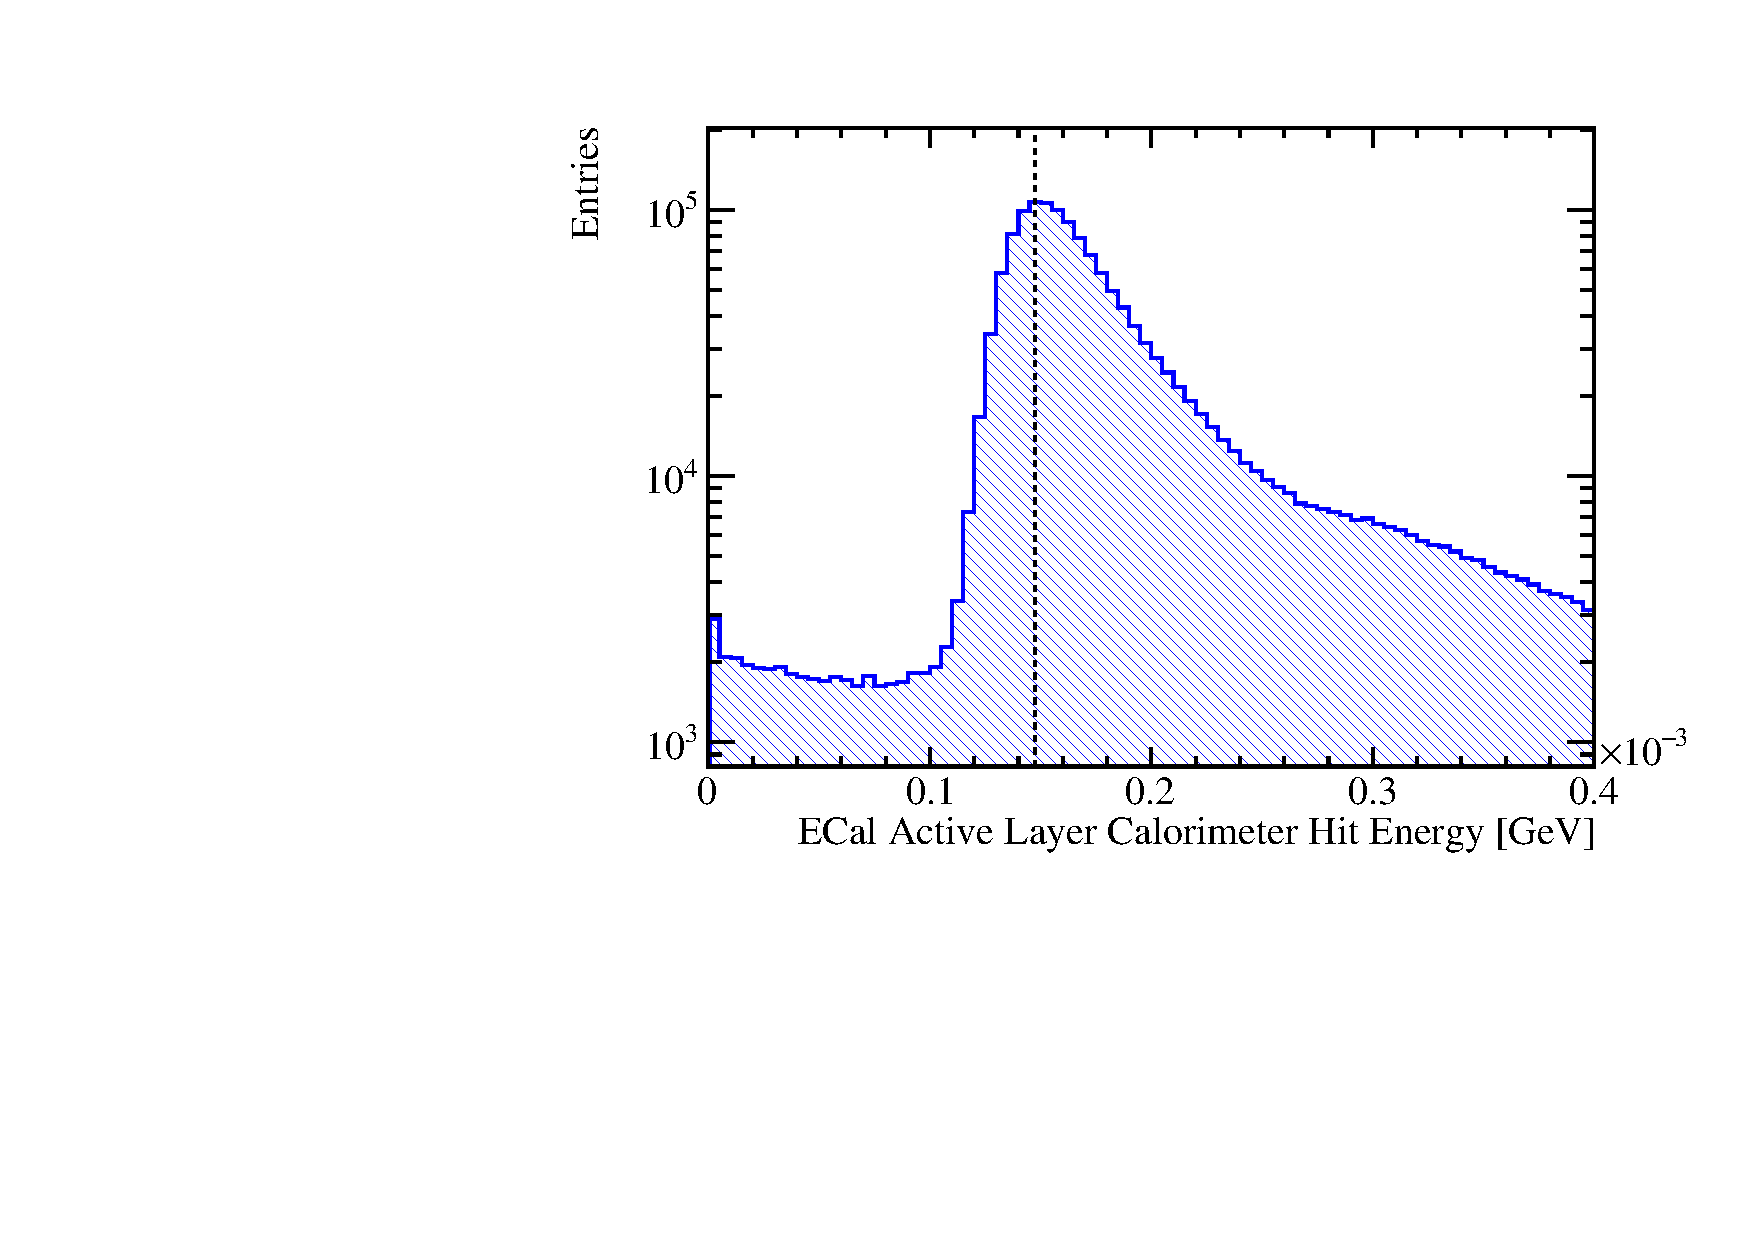
\includegraphics[width=0.5\textwidth]{EnergyEstimators/Plots/Calibration/MIPScale/Digitiser/MIPScaleDigitiserECal.pdf}}
\subfloat[]{\label{fig:digitisermiphcalbarrel}\includegraphics[width=0.5\textwidth]{EnergyEstimators/Plots/Calibration/MIPScale/Digitiser/MIPScaleDigitiserHCalbarrel.pdf}} \\
\subfloat[]{\label{fig:digitisermiphcalendcap}\includegraphics[width=0.5\textwidth]{EnergyEstimators/Plots/Calibration/MIPScale/Digitiser/MIPScaleDigitiserHCalendcap.pdf}}
\subfloat[]{\label{fig:digitisermiphcalring}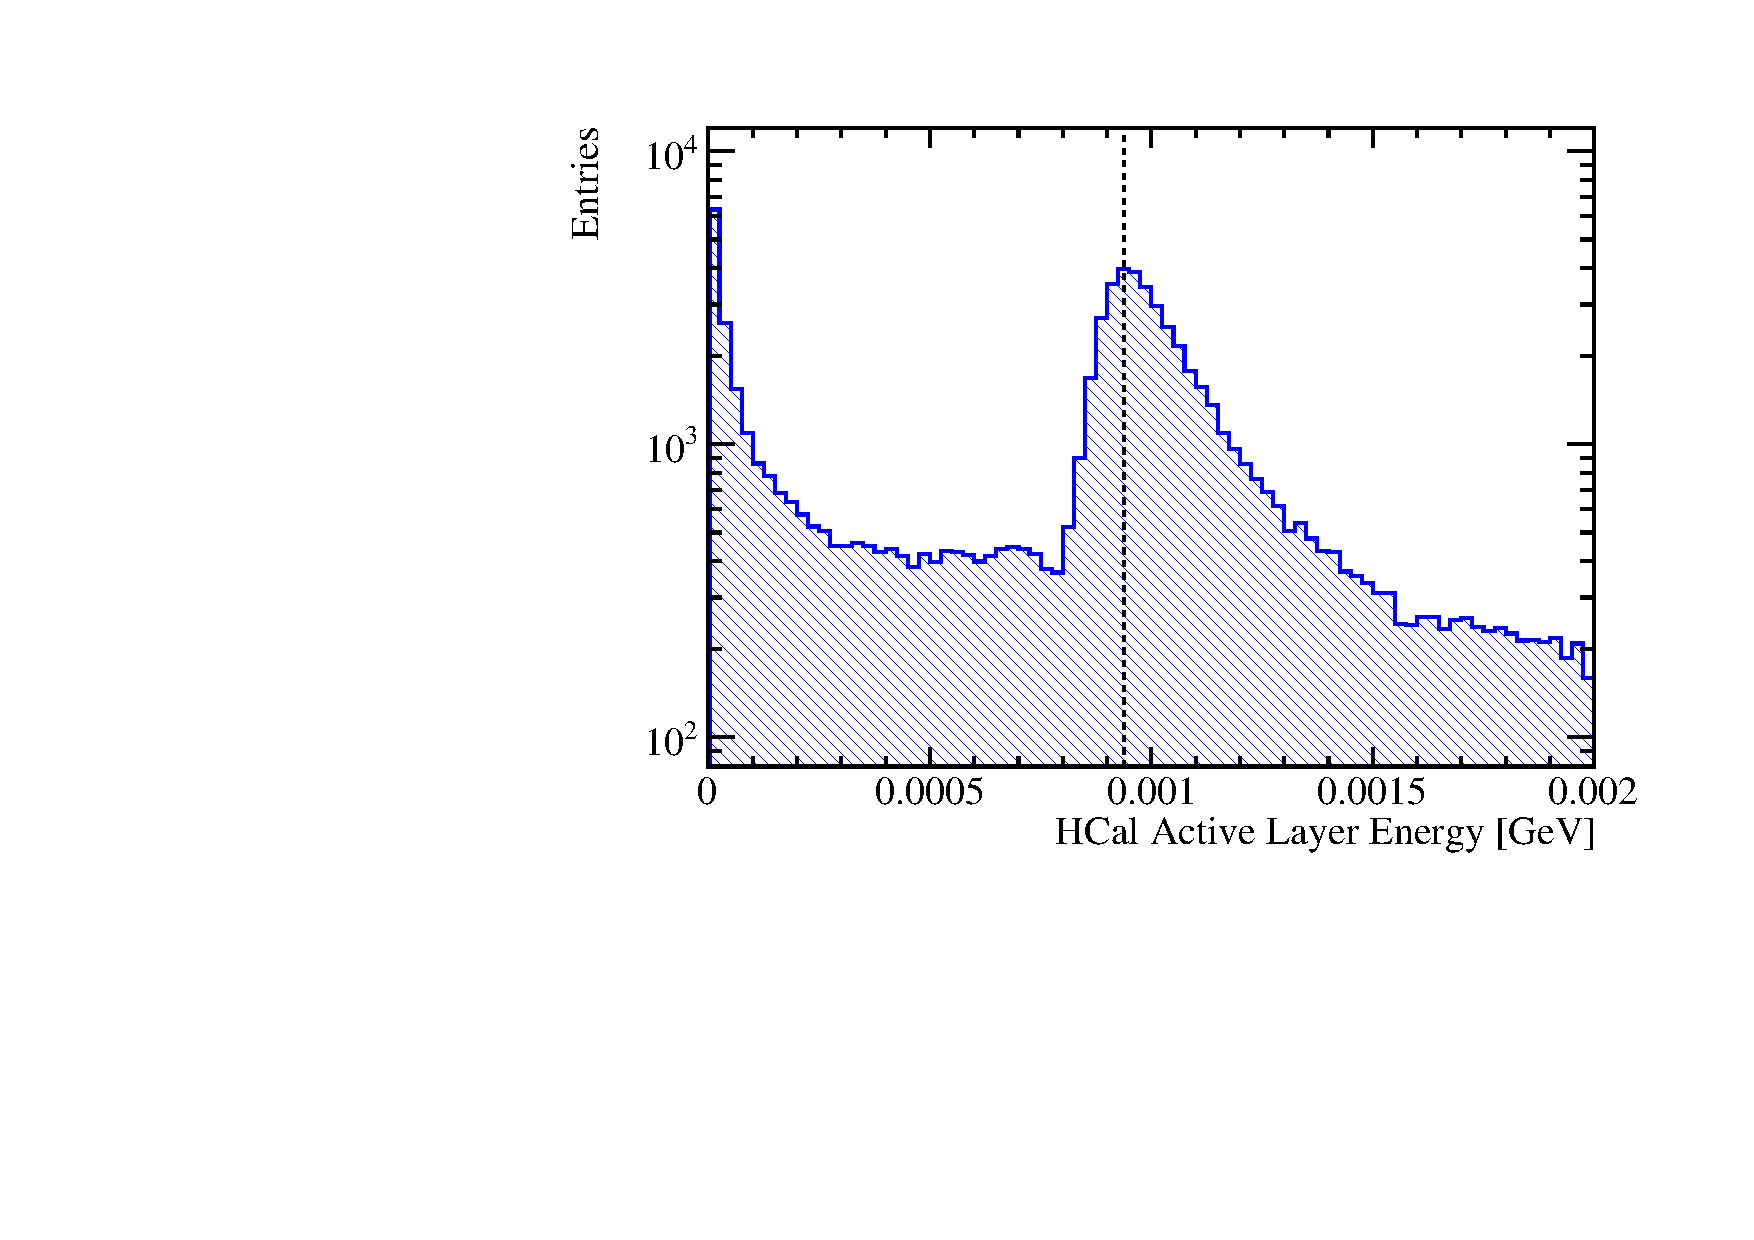
\includegraphics[width=0.5\textwidth]{EnergyEstimators/Plots/Calibration/MIPScale/Digitiser/MIPScaleDigitiserHCalOther.pdf}}
\caption[The active layer calorimeter hit energy distributions for \protect\subref{fig:digitisermipecal} the ECal, \protect\subref{fig:digitisermiphcalbarrel} the HCal barrel, \protect\subref{fig:digitisermiphcalendcap} the HCal endcap and \protect\subref{fig:digitisermiphcalring} the HCal ring for 10~GeV $\mu^{-}$ events.  The hit energies were corrected to account for the path length of the muons through the active medium of the calorimeter.  The vertical black dotted lines indicate the position of the peak in each of these distributions that is used for defining the MIP scale in the digitisation processor.]{The active layer calorimeter hit energy distributions for \protect\subref{fig:digitisermipecal} the ECal, \protect\subref{fig:digitisermiphcalbarrel} the HCal barrel, \protect\subref{fig:digitisermiphcalendcap} the HCal endcap and \protect\subref{fig:digitisermiphcalring} the HCal ring for 10~GeV $\mu^{-}$ events.  The hit energies were corrected to account for the path length of the muons through the active medium of the calorimeter.  The vertical black dotted lines indicate the position of the peak in each of these distributions that is used for defining the MIP scale in the digitisation processor.}
\label{fig:digitisermip}
\end{figure}

%========================================================================================

\subsection{Digitisation Implementation}
\label{sec:digi}
This section discusses how the digitisation constants, $\alpha$s, are determined.  The digitisation constant for a given calorimeter depends upon several factors such as the material properties of the active and absorber layers, the magnetic field strength and energy losses occurring within the gaps in the detector.  Therefore, each calorimeter in the ILD detector model has a distinct constant that must be determined independently. 

%========================================================================================

\subsubsection{ECal Digitisation Implementation}
\label{sec:ecaldigi}
The procedure for determining the digitisation constants in the ECal involves simulation of single photons at an energy $E_{MC} = 10$~GeV.  Single photons at this energy are largely contained within the ECal, as shown in figure \ref{fig:ecaldigiphotonsplit}.  This makes them ideal for isolating the ECal digitisation calibration from that of the HCal digitisation calibration.  Events are only used for calibrating the ECal digitisation if they are confined to the ECal.  To that extent, cuts are applied ensuring that the sum of the reconstructed energy found outside the ECal is less than 1\% of $E_{MC}$ and that the $\text{cos}(\theta) < 0.95$, where $\theta$ is the polar angle of the photon.  Photons that convert are also vetoed in this event sample at MC level.  The impact of these cuts on the sum of ECal hit energies for the $E_{MC} = 10$~GeV photons is shown in figure \ref{fig:ecaldigiselection}.

\begin{figure}[h!]
\subfloat[]{\label{fig:ecaldigiphotonsplit}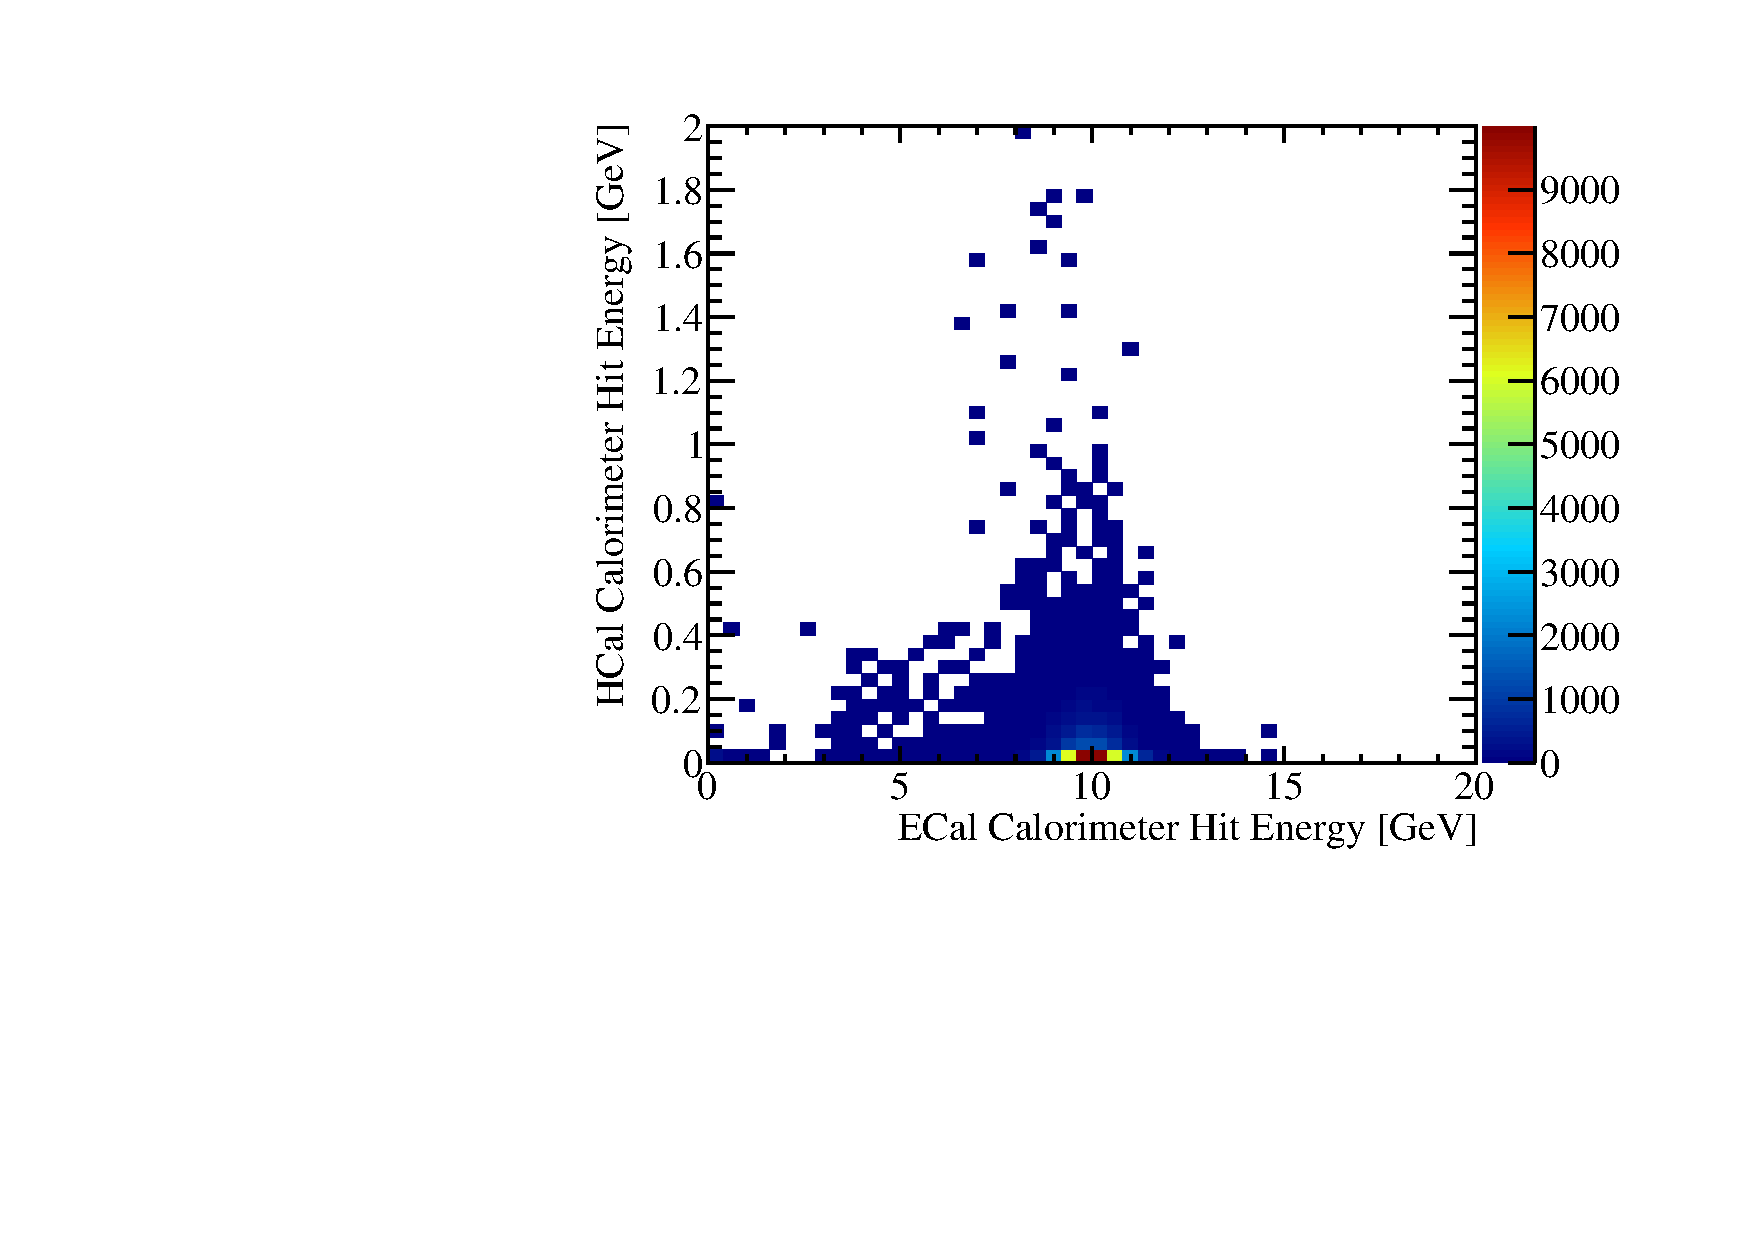
\includegraphics[width=0.5\textwidth]{EnergyEstimators/Plots/Calibration/Digitsation/ECal/ECalHCalPhotonSplit.pdf}}
\subfloat[]{\label{fig:ecaldigiselection}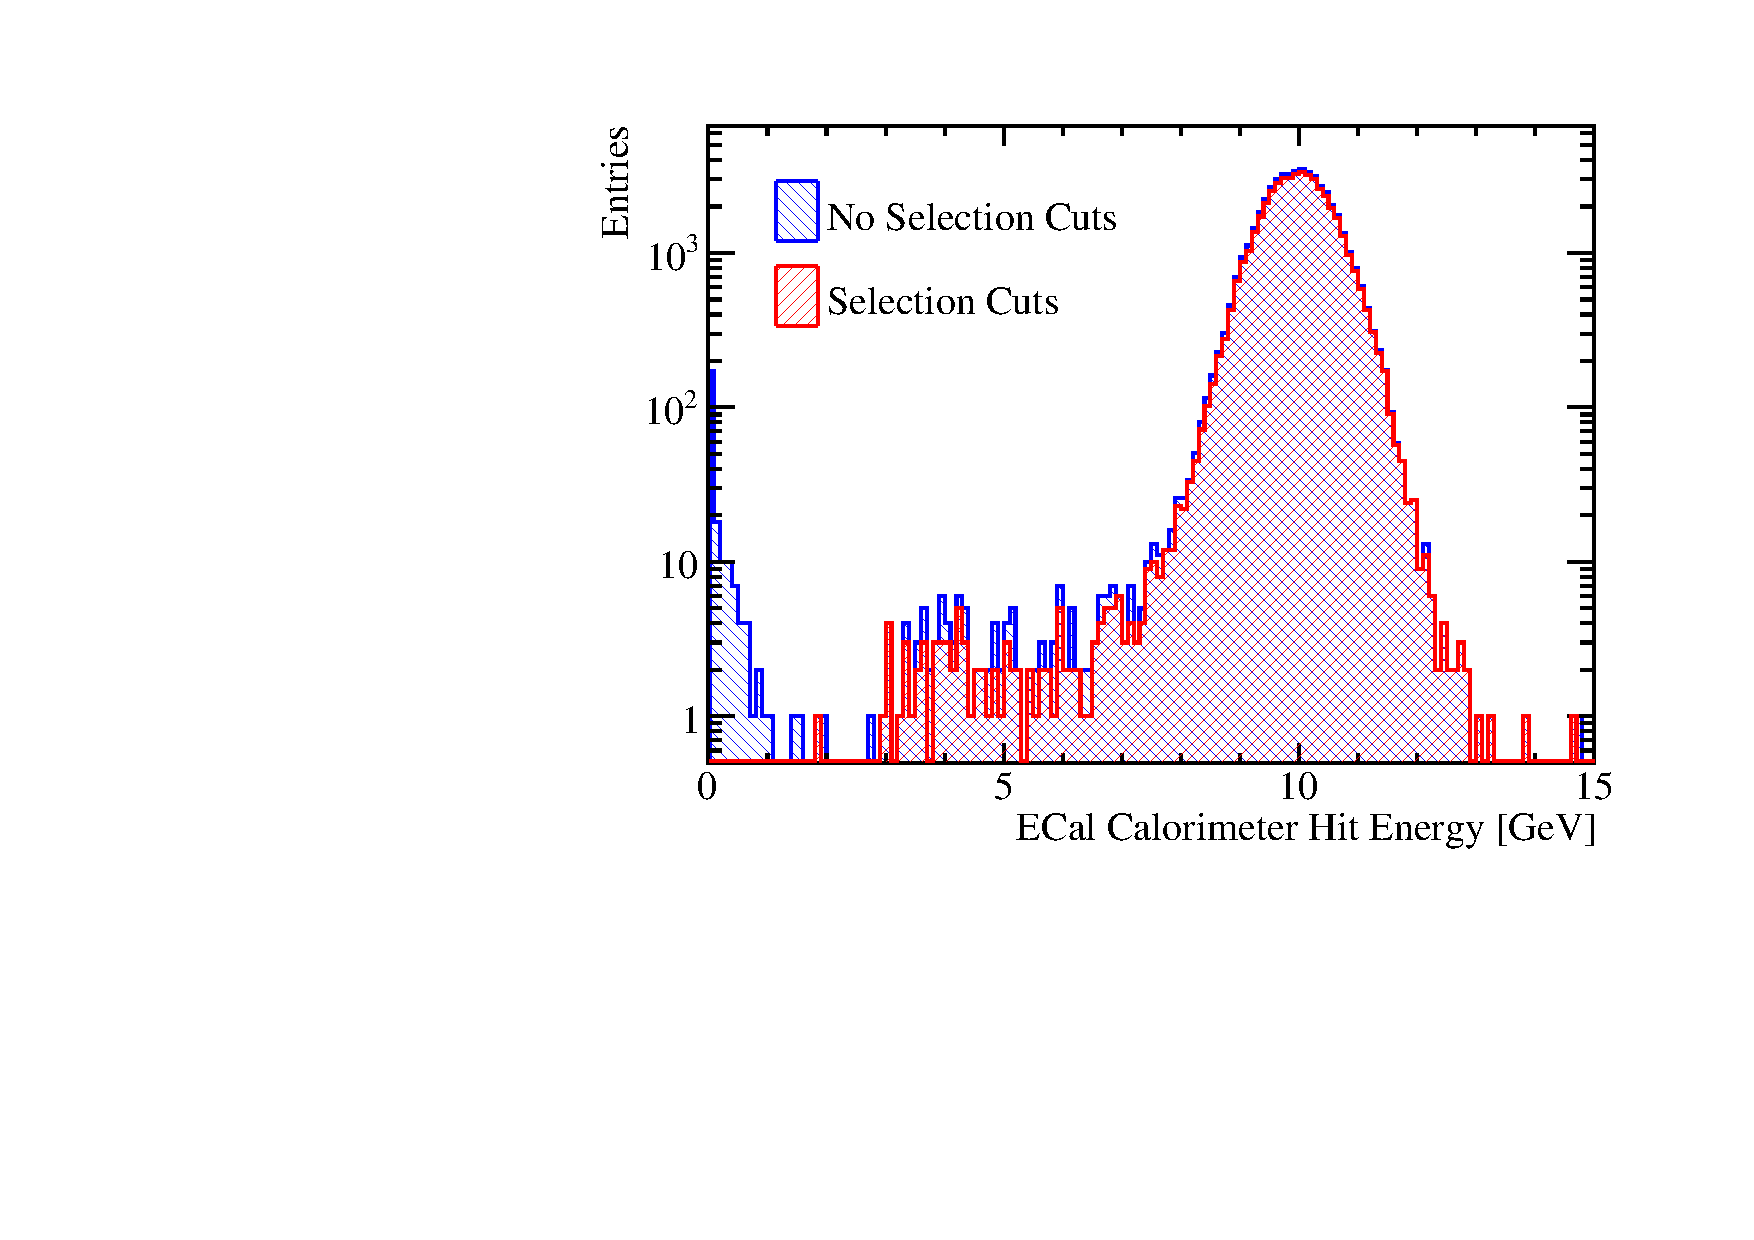
\includegraphics[width=0.5\textwidth]{EnergyEstimators/Plots/Calibration/Digitsation/ECal/DigitisationECalSelection.pdf}}
\caption[\protect\subref{fig:ecaldigiphotonsplit} The sum of calorimeter hit energies in ECal and HCal for 10~GeV photons.  \protect\subref{fig:ecaldigiselection} The sum of the ECal calorimeter hit energies for 10~GeV photons with and without the selection cuts.]{\protect\subref{fig:ecaldigiphotonsplit} The sum of calorimeter hit energies in ECal and HCal for 10~GeV photons.  \protect\subref{fig:ecaldigiselection} The sum of the ECal calorimeter hit energies for 10~GeV photons with and without the selection cuts.}
\label{fig:ecaldigi}
\end{figure}

The calibration of the digitisation in the ECal is an iterative procedure, which begins with the simulation of single photons using a trial calibration, $\alpha^{0}_{\text{ECal}}$.  Next the distribution of the sum of calorimeter hit energies within the ECal is produced for events passing the selection cuts, as shown in figure \ref{fig:ecaldigiselection}.  For an ideal calorimeter this distribution should be Gaussian, as described in chapter \ref{chap:detopt}, therefore, a Gaussian fit is applied to this distribution and the mean, $E_{\text{Fit}}$, extracted.  To remove the effect of any outliers in this distribution, the fit is applied to the range of data with the smallest root mean square that contains at least 90 \% of the data.  An example of such a fit is shown in figure \ref{fig:ecaldigifit}.  In the case of ideal calibration, the mean of this fit, $E_{\text{Fit}}$, would be equal $E_{MC}$.  It is assumed that any difference between the two is due to the calibration, therefore, to correct this the digitisation constant from the trial calibration, $\alpha^{0}_{\text{ECal}}$, is rescaled by the ratio of the $E_{MC}$ to $E_{\text{Fit}}$
%
\begin{equation}
\alpha^{0}_{\text{ECal}} \rightarrow \alpha_{\text{ECal}} = \alpha^{0}_{\text{ECal}} \times \frac{E_{MC}}{E_{Fit}}\text{ .}
\end{equation}
%
This procedure is then repeated until the $E_{\text{Fit}}$ falls within a specified tolerance of $E_{MC}$.  The tolerance applied here was $|E_{\text{Fit}} - E_{\text{MC}}| < E_{\text{MC}} \times 5 \%$.  The binning used for the fitted histogram is chosen such that the bin width is equal to the desired tolerance on $E_{\text{Fit}}$ e.g. $E_{\text{MC}} \times 5 \% = 0.5$~GeV.  It should be emphasised that the PFO energies used for downstream analyses have the electromagnetic and hadronic energy scale corrections applied, which are calibrated to a much tighter accuracy.

\begin{figure}[h!]
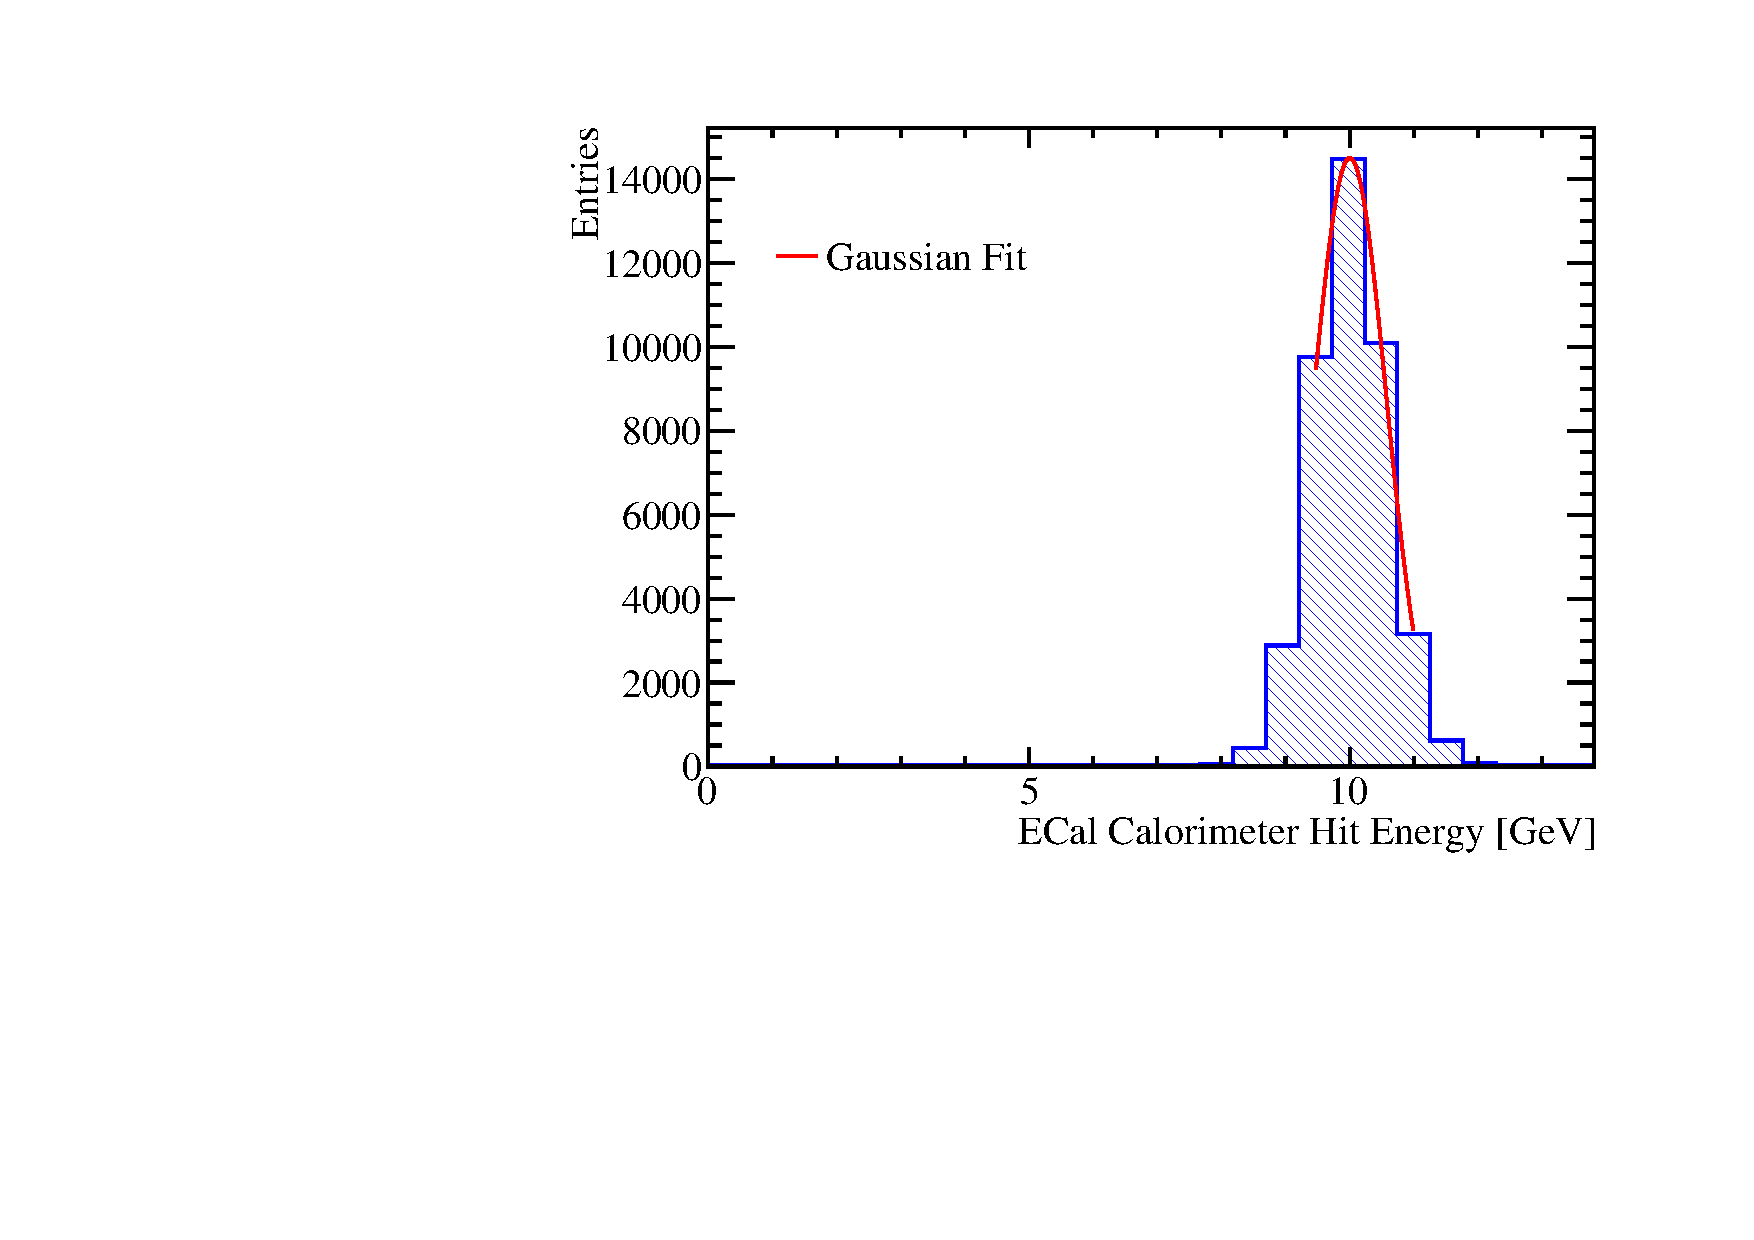
\includegraphics[width=0.5\textwidth]{EnergyEstimators/Plots/Calibration/Digitsation/ECal/DigitisationECalFit.pdf}
\caption[Gaussian fit to sum of the ECal calorimeter hit energies for 10~GeV photons with selection cuts.  The coarse binning reflects the tolerance on the digitisation constant calibration.]{Gaussian fit to sum of the ECal calorimeter hit energies for 10~GeV photons with selection cuts.  The coarse binning reflects the tolerance on the digitisation constant calibration.}
\label{fig:ecaldigifit}
\end{figure}

%========================================================================================
% 7467 out of 50000 have no ECal energy. ~ 15 %.  Negligible beampipe evts.

\subsubsection{HCal Digitisation Implementation}
\label{sec:hcaldigi}
The calibration for the digitisation in the HCal proceeds in a similar manner to that described for the ECal with a few key differences.  This calibration uses simulated MC long-lived neutral kaons ($K^{0}_{L}$s) at $E_{MC} = 20$~GeV.  The higher energy, with respect to the ECal digitisation, results in particle showers that sample deeper into the HCal.  The $K^{0}_{L}$s must pass through the ECal, which contains one $\lambda_{I}$, before arriving at the HCal.  Consequently, approximately 15\% of these events begin showering in the ECal, as can be seen in figure \ref{fig:hcaldigikaonsplit}.  Only events that deposit less than 5\% of their energy in the ECal are used for calibrating the HCal digitisation constants.  Furthermore, events that are not contained in the HCal are removed by requiring the last layer of the HCal where energy is deposited is required to be in the innermost 90\% of the HCal.  The impact of these cuts on the sum of HCal calorimeter hit energies for the $E_{MC} = 20$~GeV $K^{0}_{L}$ events is shown in figure \ref{fig:hcaldigiselection}.  

There are two HCal digitisation constants used in the detector simulation, one applied for the barrel and another for the endcap.  The use of two digitisation constants accounts for differences in hadronic shower dynamics between the two, such as differing magnetic field configurations in the barrel and endcap.  Both parameters are calibrated in the same manner, but have different cuts on $\theta$, the polar angle of the $K^{0}_{L}$.  For the barrel region of the HCal events are selected if $0.2 < \text{cos}(\theta) < 0.6$, while for the endcap events are selected if $0.8 < \text{cos}(\theta) < 0.9$.  These angular cuts account for the transverse profile of the hadronic showers and ensure that the showers are largely confined to the relevant sub-detector.  As many of the neutral hadrons appearing in jets are neutrons and their accessible energy is the kinetic energy as opposed to the total energy, the target reconstructed energy for these $K^{0}_{L}$ samples is the kinetic energy.  

\begin{figure}[h!]
\subfloat[]{\label{fig:hcaldigikaonsplit}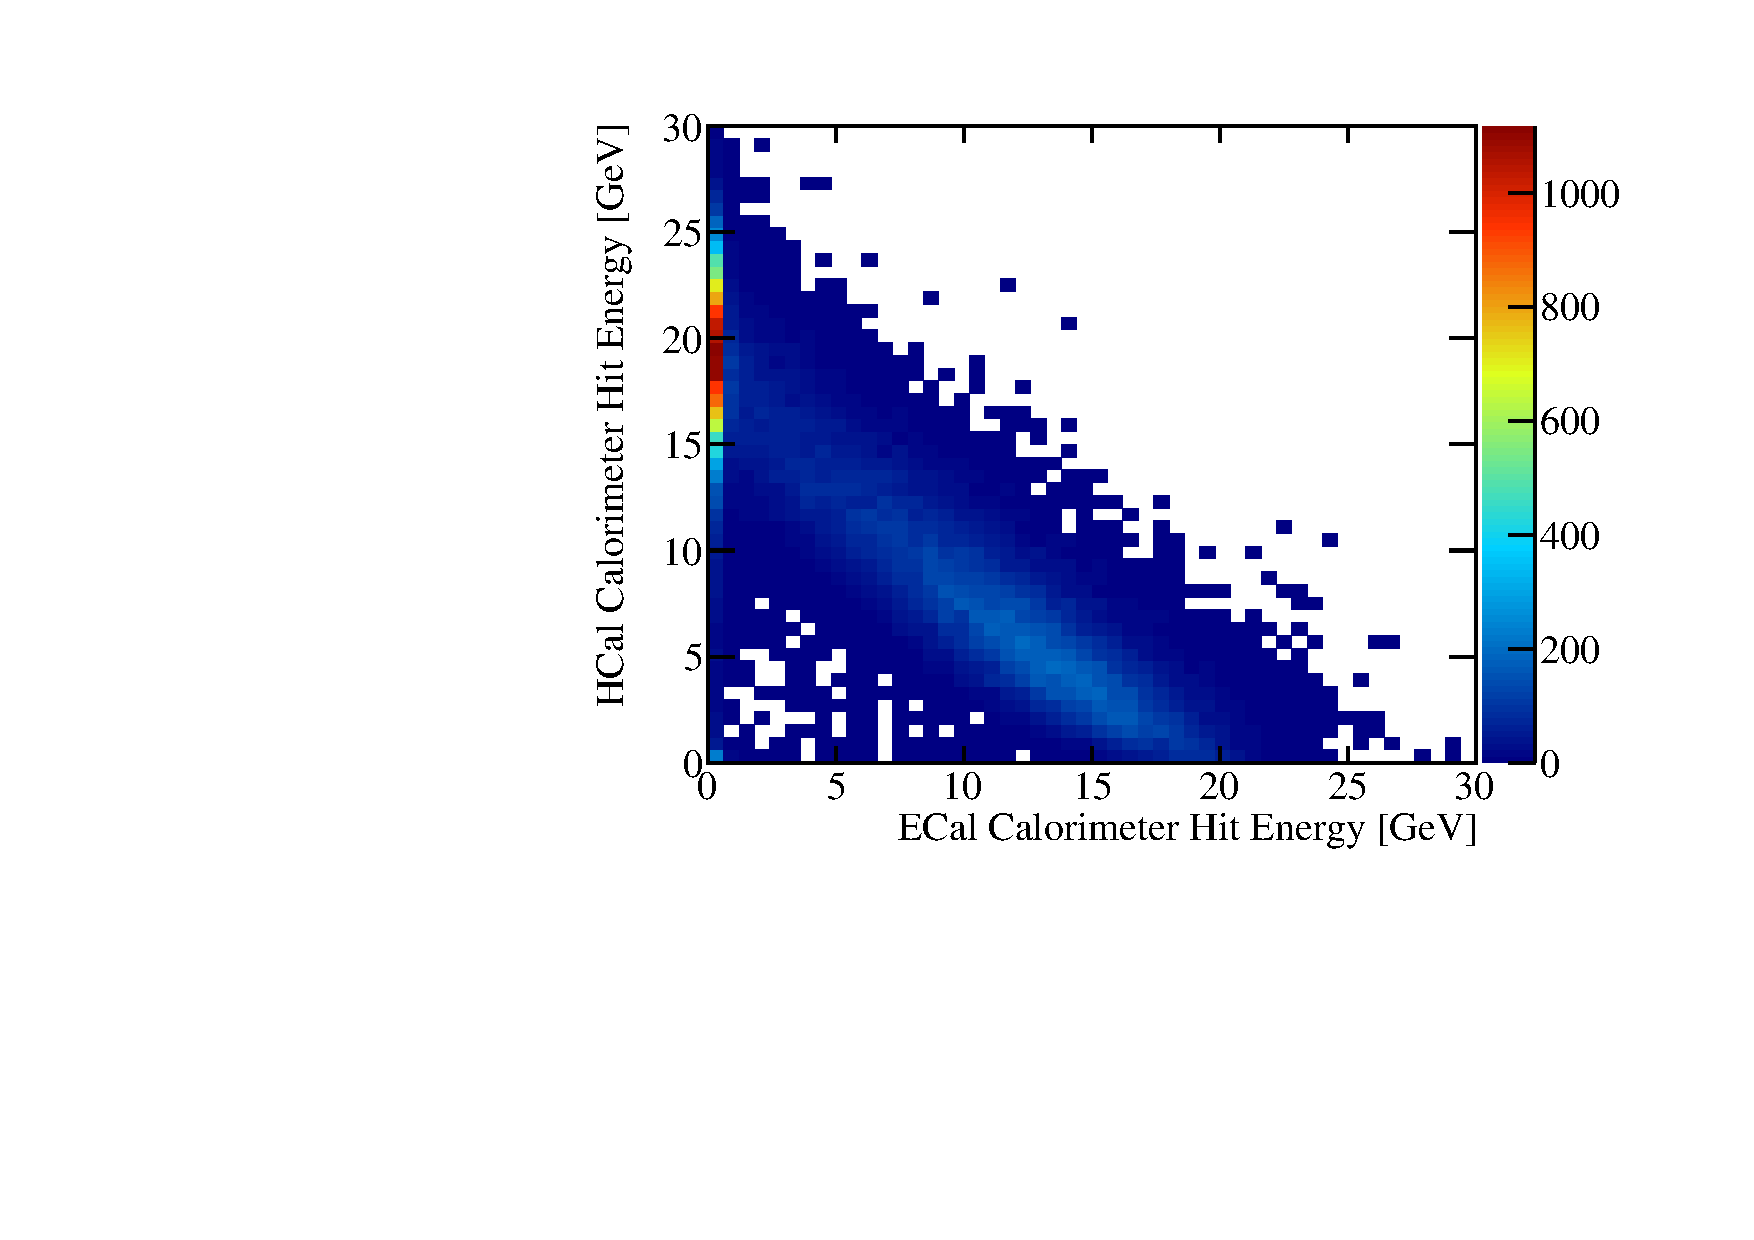
\includegraphics[width=0.5\textwidth]{EnergyEstimators/Plots/Calibration/Digitsation/HCal/ECalHCalKaon0LSplit.pdf}}
\subfloat[]{\label{fig:hcaldigiselection}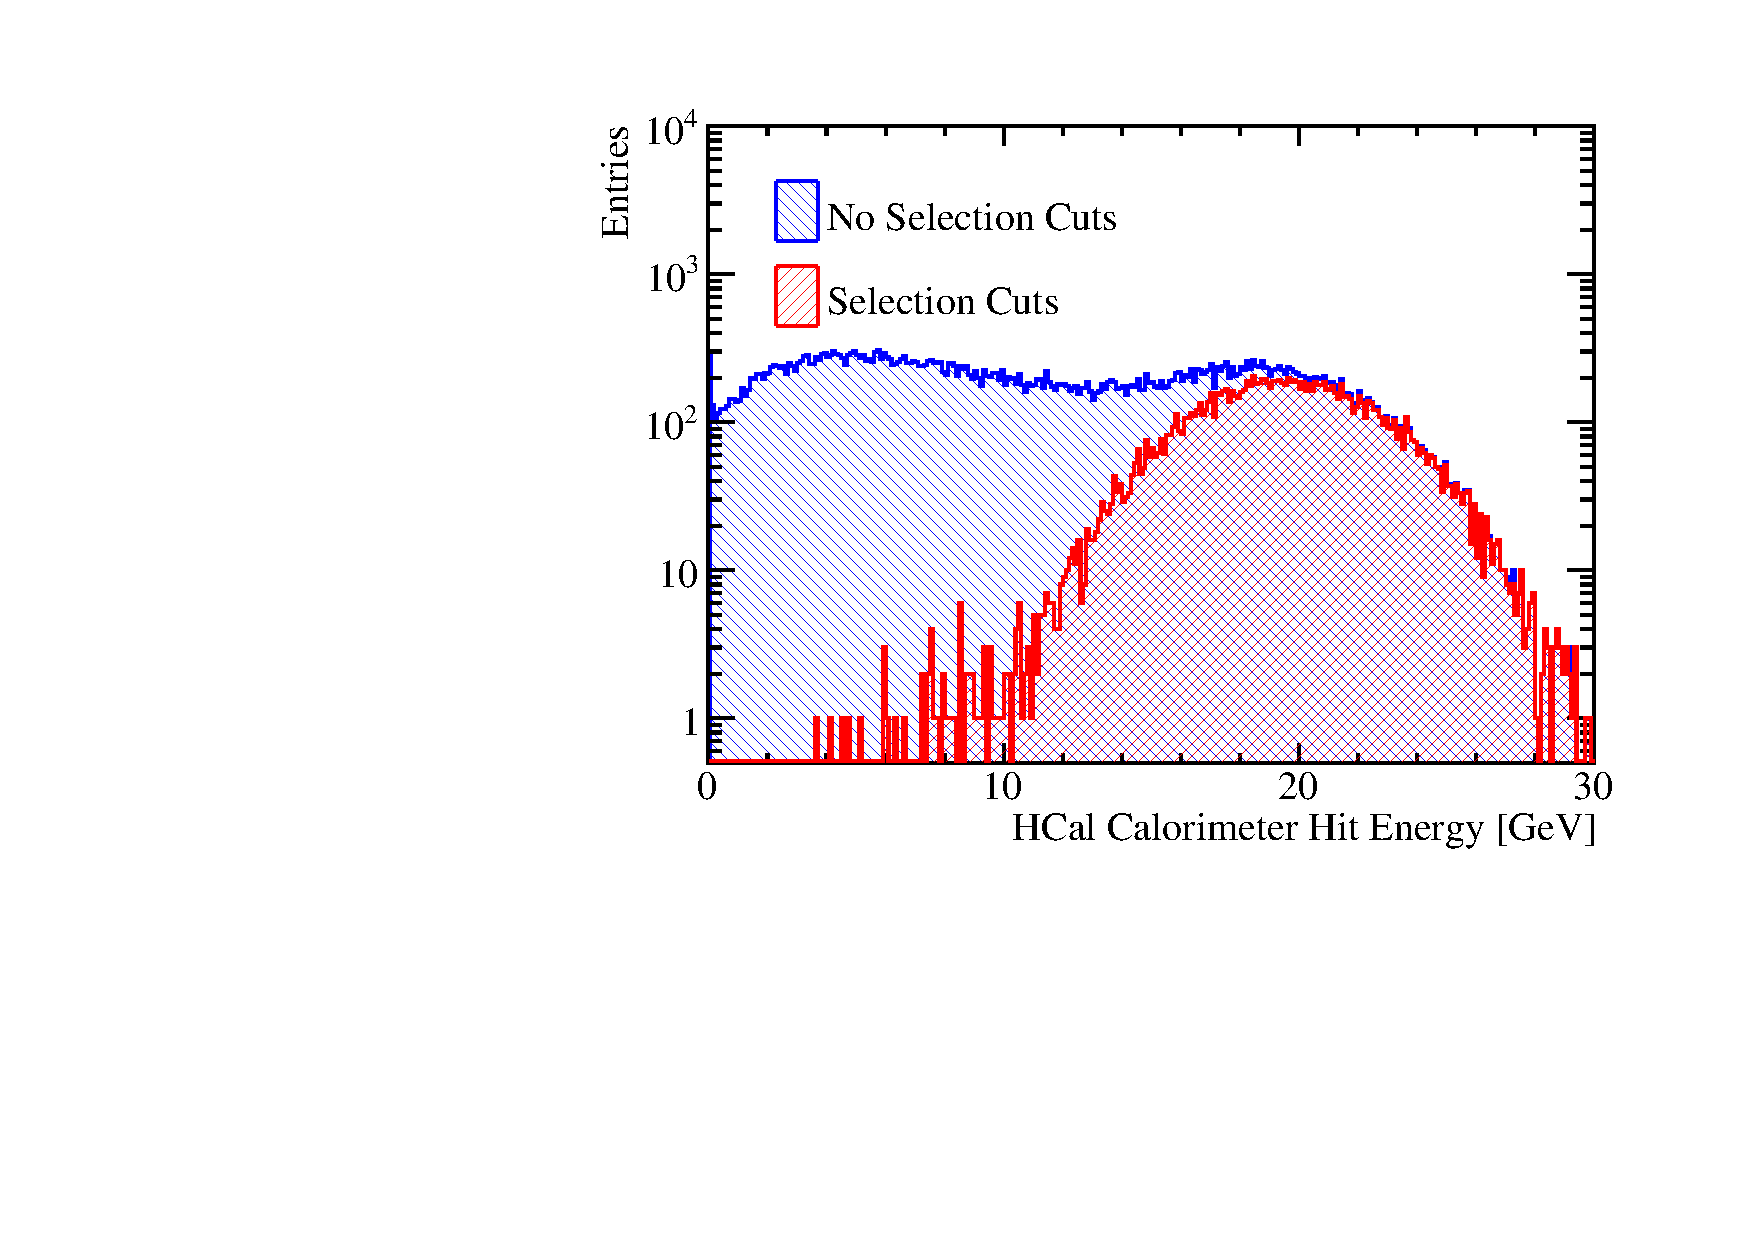
\includegraphics[width=0.5\textwidth]{EnergyEstimators/Plots/Calibration/Digitsation/HCal/DigitisationHCalSelection.pdf}}
\caption[\protect\subref{fig:hcaldigikaonsplit} Sum of calorimeter hit energies in ECal and HCal for 20~GeV $K^{0}_{L}$ events.  \protect\subref{fig:hcaldigiselection} Sum of the HCal calorimeter hit energies for a 20~GeV $K^{0}_{L}$ events with and without the selection cuts.]{\protect\subref{fig:hcaldigikaonsplit} Sum of calorimeter hit energies in ECal and HCal for 20~GeV $K^{0}_{L}$ events.  \protect\subref{fig:hcaldigiselection} Sum of the HCal calorimeter hit energies for a 20~GeV $K^{0}_{L}$ events with and without the selection cuts.}
\label{fig:hcaldigi}
\end{figure}

After applying the above $K^{0}_{L}$ selection cuts, the calibration procedure for the digitisation of the HCal barrel and endcap proceeds in the same manner as was described for the ECal.  An example of the Gaussian fits applied to the sum of the calorimeter hit energies in the HCal barrel and endcap are shown in figure \ref{fig:hcaldigifit}.  

\begin{figure}[h!]
\subfloat[HCal barrel.]{\label{fig:hcaldigibarrel}\includegraphics[width=0.5\textwidth]{EnergyEstimators/Plots/Calibration/Digitsation/HCal/DigitisationHCalbarrelFit.pdf}}
\subfloat[HCal endcap.]{\label{fig:hcaldigiendcap}\includegraphics[width=0.5\textwidth]{EnergyEstimators/Plots/Calibration/Digitsation/HCal/DigitisationHCalendcapFit.pdf}}
\caption[Gaussian fit to sum of the HCal calorimeter hit energies for 20~GeV $K^{0}_{L}$ events with selection cuts.]{Gaussian fit to sum of the HCal calorimeter hit energies for 20~GeV $K^{0}_{L}$ events with selection cuts.}
\label{fig:hcaldigifit}
\end{figure}

%========================================================================================

\subsubsection{HCal Ring Digitisation Implementation}
\label{sec:hcalringdigi}
The HCal ring, as illustrated in figure \ref{fig:calorimeters}, is a hadronic calorimeter that surrounds the ECal endcap and is sandwiched between the HCal barrel and endcap.  This calorimeter is required to ensure hermetic coverage of the hadronic calorimeter system across the barrel/endcap cross-over region \cite{Behnke:2013lya}.  

The HCal ring has an independent digitisation constant to account for any difference in the hadronic shower development between the ring, barrel and endcap.  Due to the thickness of the HCal ring, particle showers are never fully contained in it, so a different approach to calibration is required.  To ensure that the HCal ring calibration is approximately correct, $\alpha_{\text{HCal ring}}$ is assumed to equal $\alpha_{\text{HCal endcap}}$ multiplied by several factors designed to account for differences in the active layer thickness, absorber layer thickness and the MIP response between the HCal endcap and ring.  In detail
%
\begin{equation}
\alpha_{\text{HCal ring}} = \alpha_{\text{HCal endcap}} \times \frac{\langle \text{cos}(\theta_\text{endcap}) \rangle}{\langle \text{cos}(\theta_\text{ring}) \rangle} \times \frac{P_\text{endcap} }{P_\text{ring} } \times \frac{L^{Absorber}_\text{endcap}}{L^{Absorber}_\text{ring} } \times \frac{L^{Active}_\text{ring}}{L^{Active}_\text{endcap}} \text{ ,}
\end{equation}
%
\noindent where $\theta$ is the incident angle of the incoming particle to the calorimeter determined using the 20~GeV $K^{0}_{L}$s, $L^{Active}$ is the active layer thickness and $L^{Absorber}$ is the absorber layer thickness.  $P$ is the position of the MIP peak in the distribution of active layer hit energies, which has been corrected so that the MIP appears to enter the calorimeter at normal incidence, and is determined using 10~GeV $\mu^{-}$ events.

\begin{figure}[h!]
\subfloat[]{\label{fig:ecal}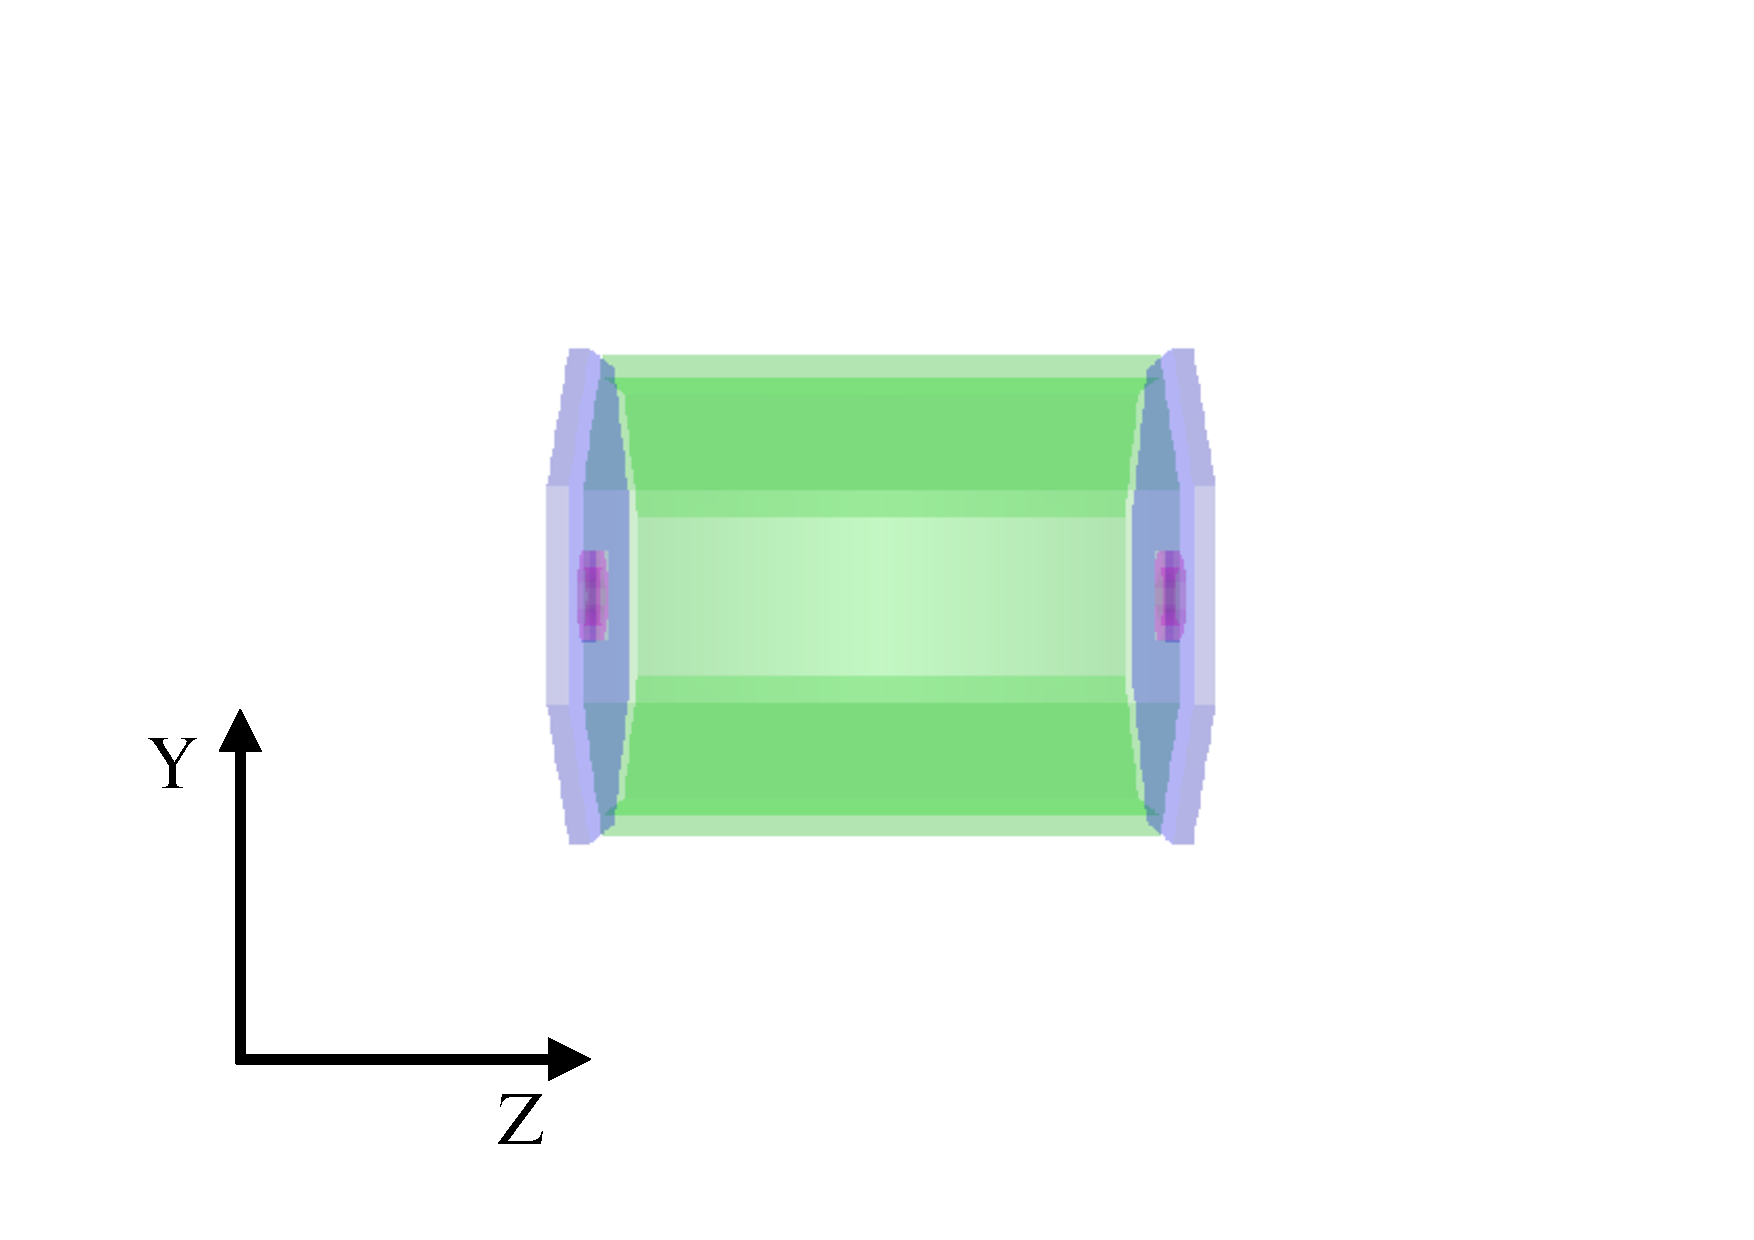
\includegraphics[width=0.33\textwidth]{EnergyEstimators/Plots/Calibration/VisualDisplay/ECalWithScale.pdf}}
\subfloat[]{\label{fig:hcal}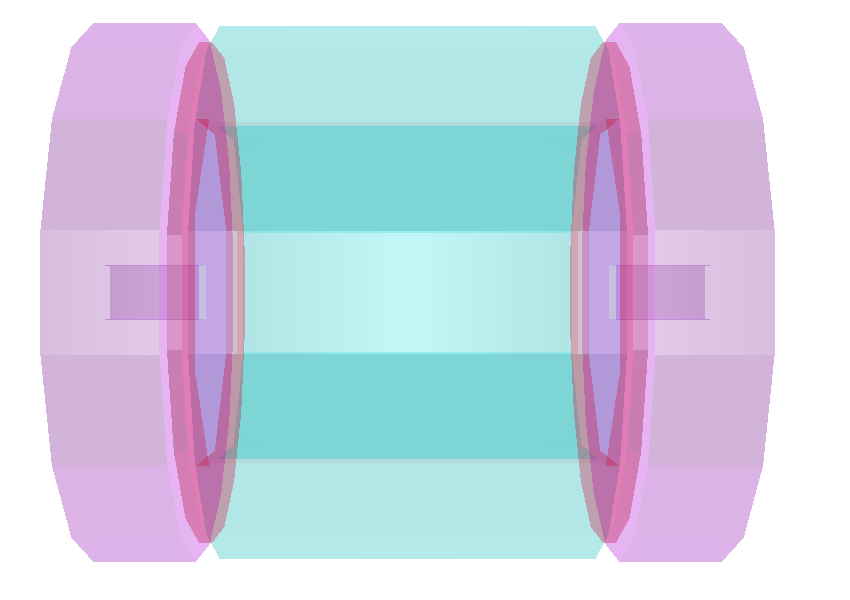
\includegraphics[width=0.33\textwidth]{EnergyEstimators/Plots/Calibration/VisualDisplay/HCal.png}}
\subfloat[]{\label{fig:hcalring}\includegraphics[width=0.33\textwidth]{EnergyEstimators/Plots/Calibration/VisualDisplay/HCalring.png}}
\caption[A PandoraPFA event display showing the nominal ILD calorimeters.  \protect\subref{fig:ecal} the ECal, \protect\subref{fig:hcal} the full HCal and \protect\subref{fig:hcalring} the HCal ring, which covers the barrel/endcap cross-over region.]{A PandoraPFA event display showing the nominal ILD calorimeters.  \protect\subref{fig:ecal} the ECal, \protect\subref{fig:hcal} the full HCal and \protect\subref{fig:hcalring} the HCal ring, which covers the barrel/endcap cross-over region.}
\label{fig:calorimeters}
\end{figure}

%========================================================================================

\subsection{MIP Scale Determination in PandoraPFA}
The MIP scale in PandoraPFA is set by simulating 10~GeV $\mu^{-}$ events and creating the distribution of combined calorimeter hit energies.  The MIP scale in PandoraPFA must to be determined for the calorimeters and, in contrast to the digitiser, the muon chamber.  Consequently, an additional distribution showing the calorimeter hit energy for the muon chamber must be constructed at this stage of the calibration.  As was done for the digitiser, a direction correction factor was applied to the hit energies account for the path length of the MIP through the active medium of the calorimeter and no selection cuts were applied.  

Examples of the distributions used to set the MIP scale in PandoraPFA can be found in figure \ref{fig:pandoramip}.  Due to the energy thresholds applied in the digitiser, there are fewer populated bins with low hit energies.  The double peak structure observed in the ECal calorimeter hit energy distribution is expected given the ECal absorber material thickness doubling in the back 10 layers of the ECal.  The MIP peaks used for defining the MIP scale in PandoraPFA, figure \ref{fig:pandoramip}, are broader than those used for determining MIP scale setting in the digitiser, \ref{fig:digitisermip}, as the realistic effects applied by the digitiser are only present in the combined calorimeter hit energy distributions.  

\begin{figure}[h!]
\subfloat[]{\label{fig:pandoramipecal}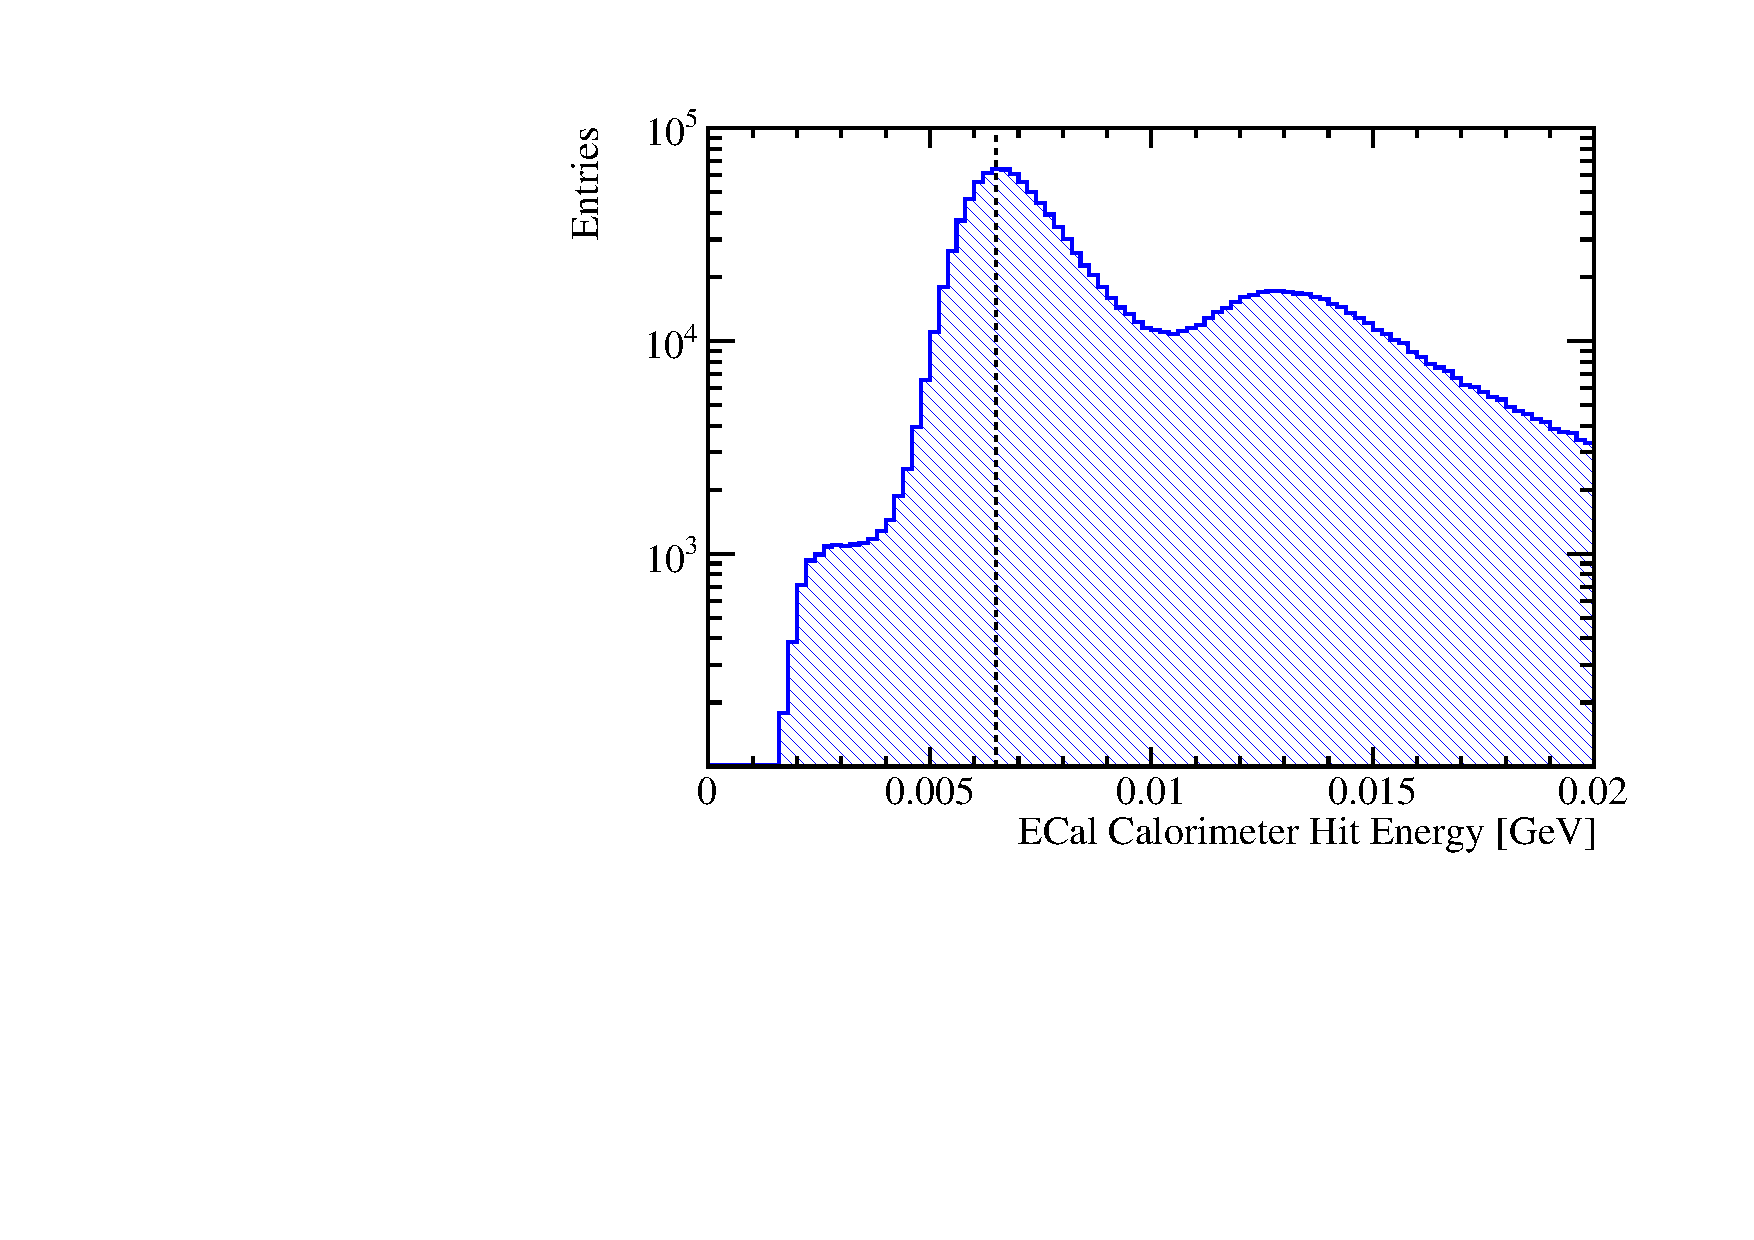
\includegraphics[width=0.5\textwidth]{EnergyEstimators/Plots/Calibration/MIPScale/PandoraPFA/MIPScalePandoraPFAECal.pdf}}
\subfloat[]{\label{fig:pandoramiphcal}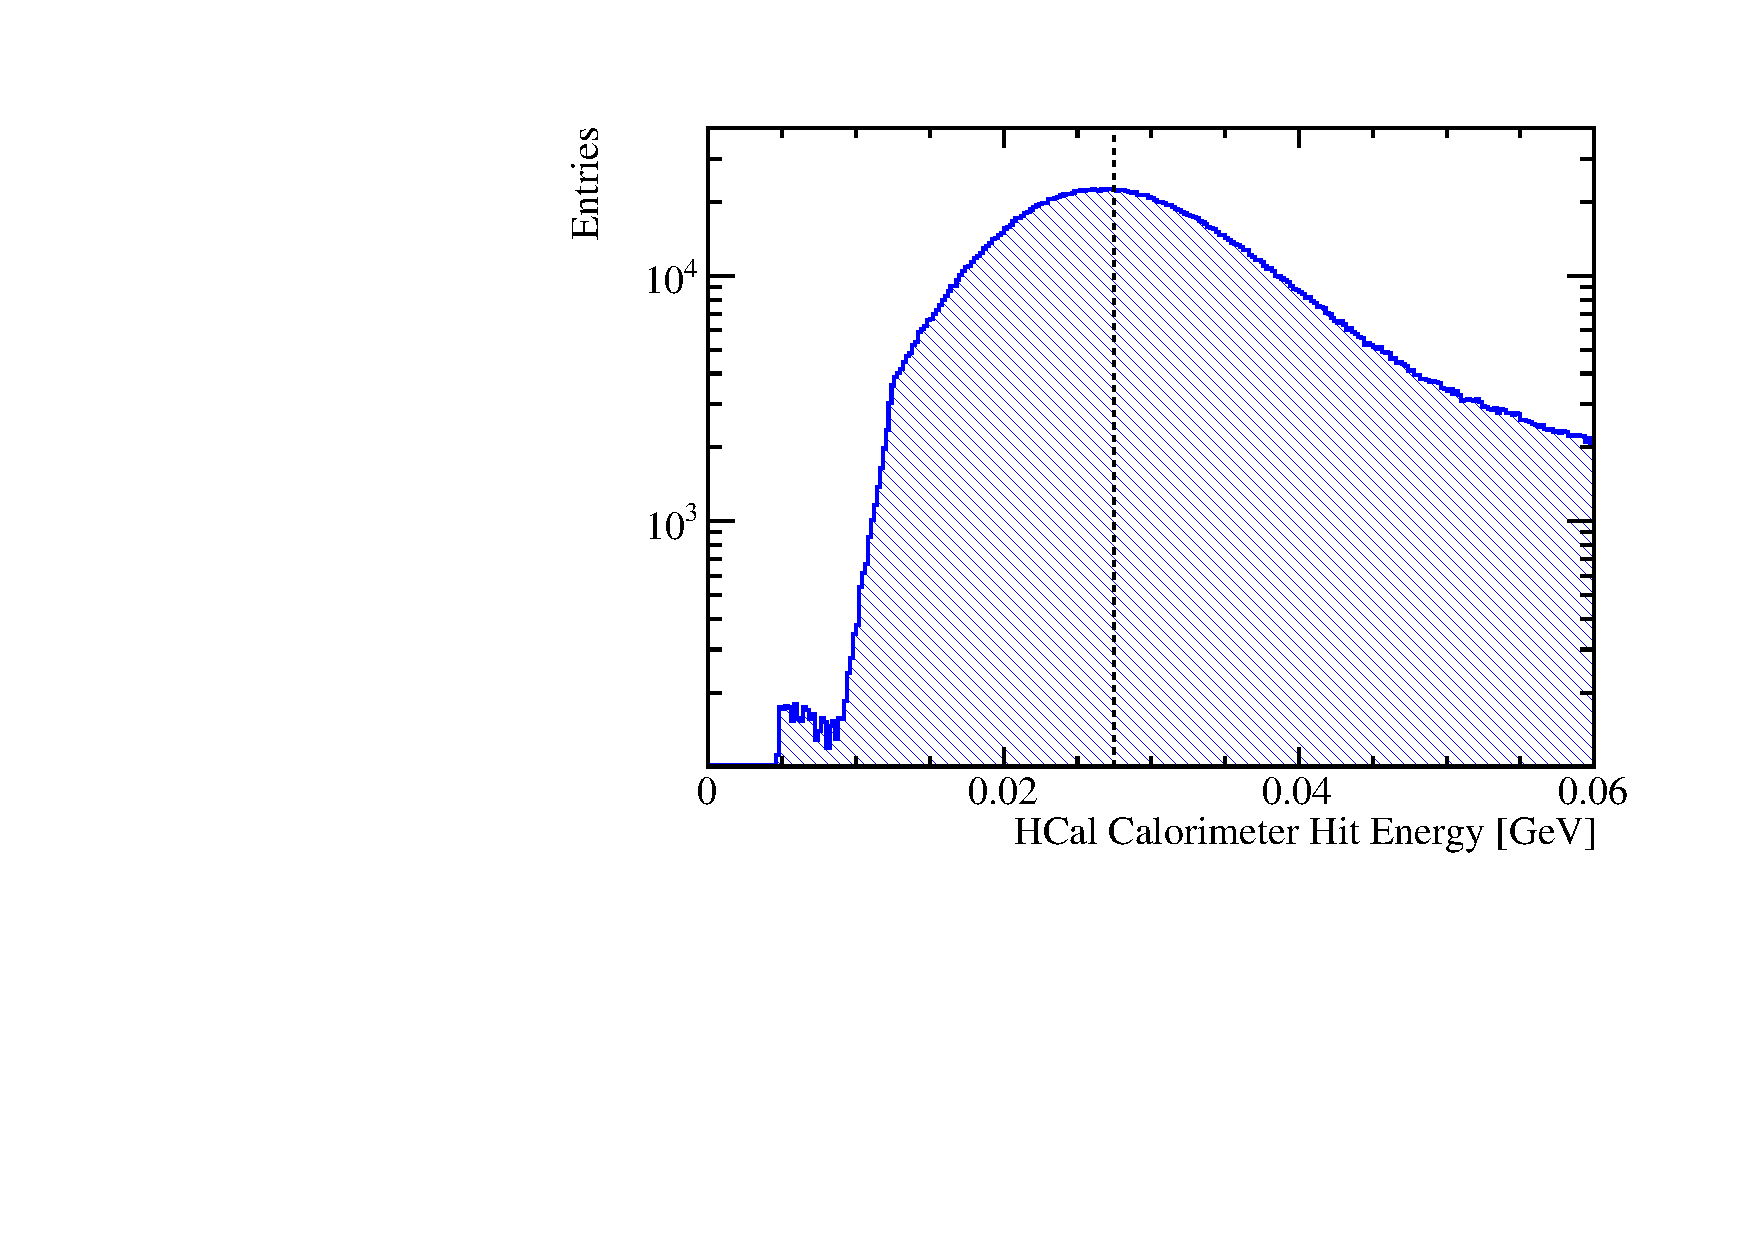
\includegraphics[width=0.5\textwidth]{EnergyEstimators/Plots/Calibration/MIPScale/PandoraPFA/MIPScalePandoraPFAHCal.pdf}} \\
\subfloat[]{\label{fig:pandoramipmuon}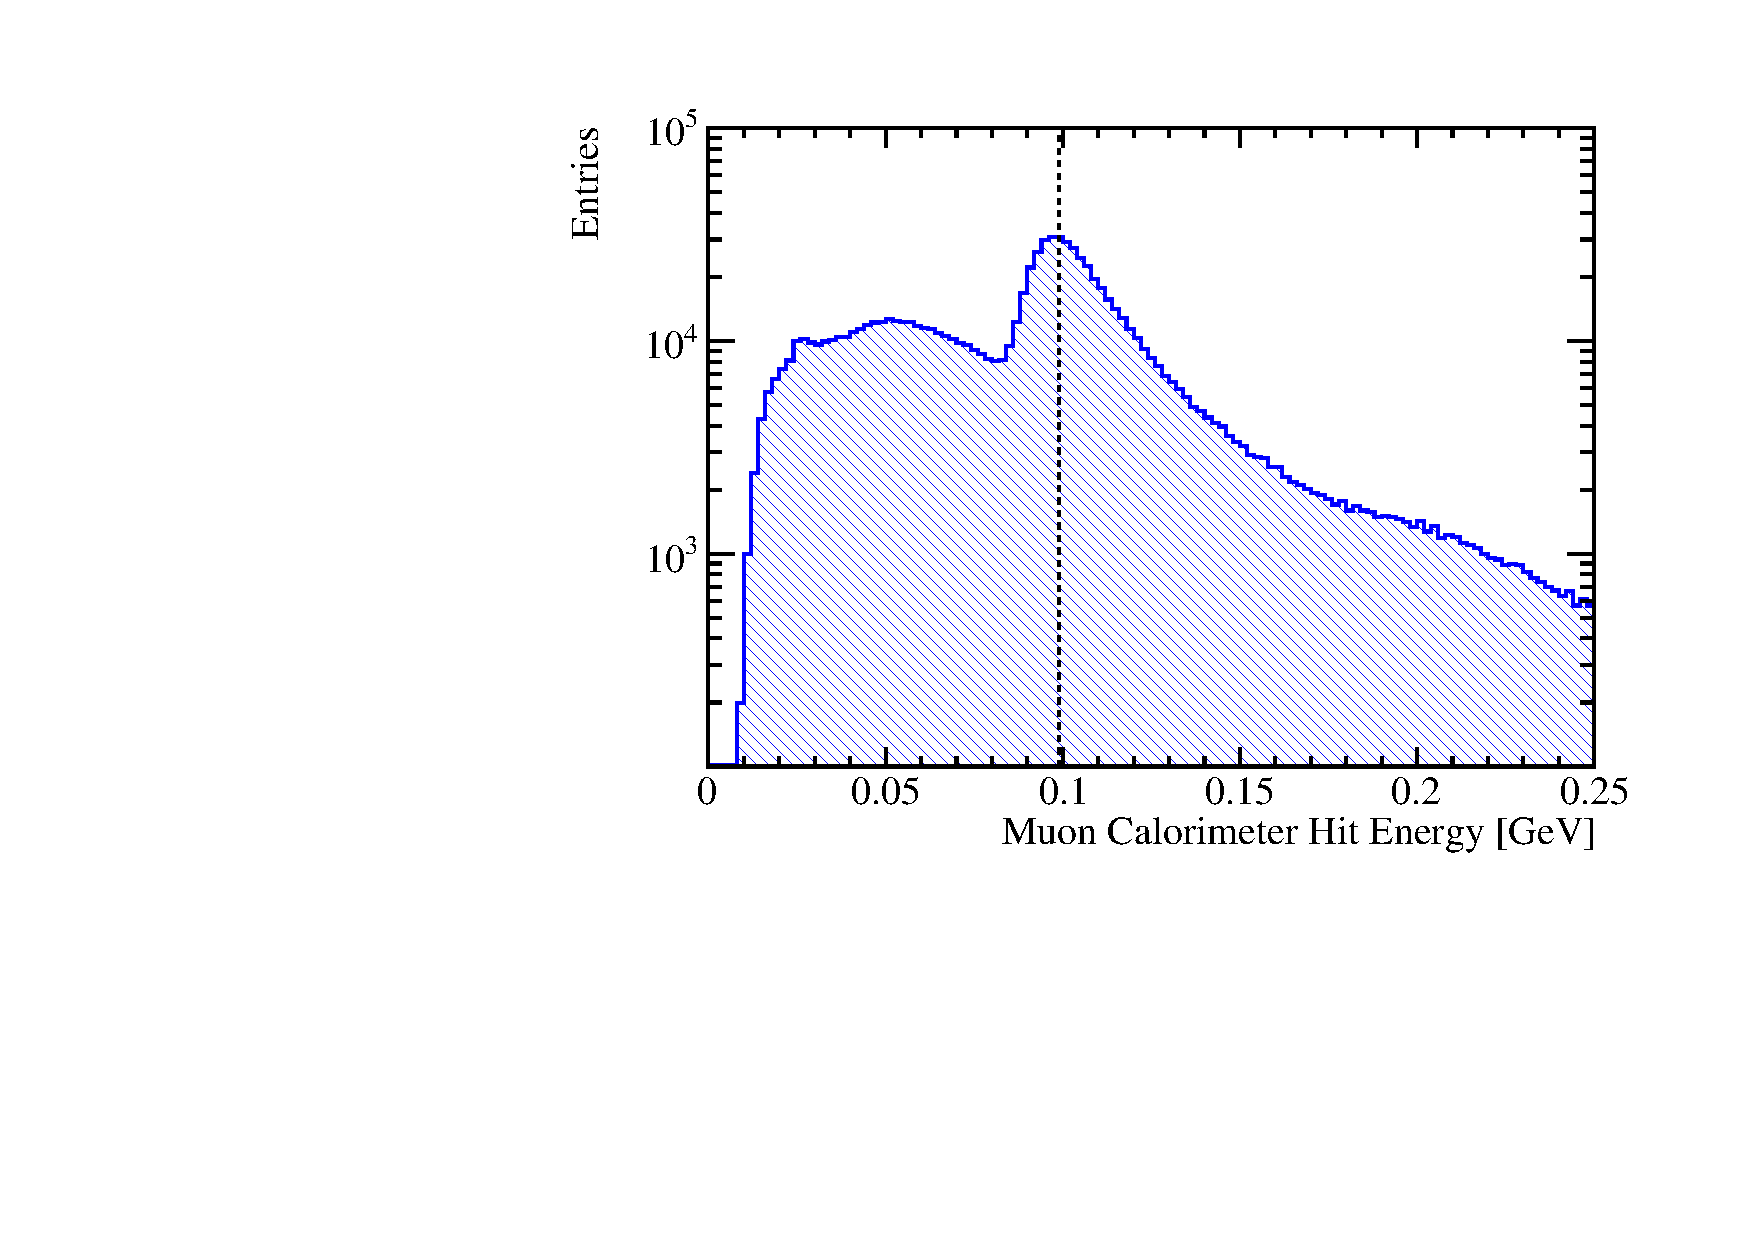
\includegraphics[width=0.5\textwidth]{EnergyEstimators/Plots/Calibration/MIPScale/PandoraPFA/MIPScalePandoraPFAMuon.pdf}}
\caption[The combined calorimeter hit energy distributions for \protect\subref{fig:pandoramipecal} the ECal, \protect\subref{fig:pandoramiphcal} the HCal and \protect\subref{fig:pandoramipmuon} the muon chamber for 10~GeV $\mu^{-}$ events.  These hit energies were corrected to account for the path length of the muons through the active medium of the calorimeter.  The vertical black dotted lines indicate the position of the peak in each of these distributions that is used for defining the MIP scale in PandoraPFA.]{The combined calorimeter hit energy distributions for \protect\subref{fig:pandoramipecal} the ECal, \protect\subref{fig:pandoramiphcal} the HCal and \protect\subref{fig:pandoramipmuon} the muon chamber for 10~GeV $\mu^{-}$ events.  These hit energies were corrected to account for the path length of the muons through the active medium of the calorimeter.  The vertical black dotted lines indicate the position of the peak in each of these distributions that is used for defining the MIP scale in PandoraPFA.}
\label{fig:pandoramip}
\end{figure}

%========================================================================================

\subsection{Electromagnetic Scale in PandoraPFA}
\label{sec:emscalesetting}
Setting the electromagnetic scale in PandoraPFA is performed by examining the energies of particles reconstructed by PandoraPFA.  The reconstruction is performed using the combined calorimeter hit energies that were set by the digitiser and having applied the noise vetoing MIP cuts.  

The electromagnetic scale in the ECal, $\beta^{EM}_{ECal}$, is determined using simulated photons at $E_{MC} = 10$~GeV.  To ensure that the events used for this part of the calibration are largely confined to the ECal, a cut requiring less than 1\% of the reconstructed energy to be found outside the ECal is applied.  Furthermore, only events reconstructed as a single photon are used to veto conversions.  The impact of the selection cuts on the electromagnetic energy measured in the ECal for 10~GeV photons is shown in figure \ref{fig:ecalemscaleselection}.  The peak at zero electromagnetic energy in the ECal is due to events traveling down the beam pipe and photon conversions.  In photon conversion events, the calorimetric energy deposits made by the $\text{e}^{\pm}$ are associated to charged particle tracks.  In this case, the energy measured using the calorimeters will be reported as zero because the charged particle tracks are used to determining the reconstructed particle energies.  The tail of events with low electromagnetic energy in the ECal occurs primarily due pattern recognition failures in photon conversion events.  In these events a small fraction of the calorimetric energy deposits made by the $\text{e}^{\pm}$ are not associated to charged particle tracks and instead are reconstructed as separate photons with a reconstructed energy much less than $E_{MC}$.

The fitting procedure follows that used for the ECal digitisation, described in section \ref{sec:ecaldigi}, whereby a trial calibration for the electromagnetic energy scale in the ECal, $\beta^{EM0}_{ECal}$, is first assumed.  The initial trial calibration is approximate and is iteratively updated until it converges to within a chosen tolerance.  Using the trial calibration, the photons are reconstructed and the distribution of the electromagnetic energy in the ECal created.  A Gaussian fit is then applied to this distribution in the range with the smallest root mean square containing at least 90 \% of the data.  The mean of the fitted Gaussian, $E_{\text{Fit}}$, is then used to scale $\beta^{EM0}_{ECal}$ in the following way
%
\begin{equation}
\beta^{EM0}_{ECal} \rightarrow \beta^{EM}_{ECal} = \beta^{EM0}_{ECal} \times \frac{E_{MC}}{E_{Fit}}\text{ .}
\end{equation}
%
An example distribution and fit used in the calibration of the nominal ILD detector model can be found in figure \ref{fig:ecalemscalefit}.  This procedure is repeated using the updated $\beta^{EM}_{ECal}$ until $E_{\text{Fit}}$ falls within a specified tolerance.  The tolerance applied here was $|E_{\text{Fit}} - E_{\text{MC}}| < E_{\text{MC}} \times 0.5 \%$.  The binning for the fitted histogram is chosen such that the bin width is equal to the desired target tolerance on $E_{\text{Fit}}$, e.g. $E_{\text{MC}} \times 0.5 \% = 0.05$~GeV.  This tolerance is tighter than was applied for the digitisation as it is these and only these energies that are used in downstream analyses.   
 
\begin{figure}[h!]
\subfloat[]{\label{fig:ecalemscaleselection}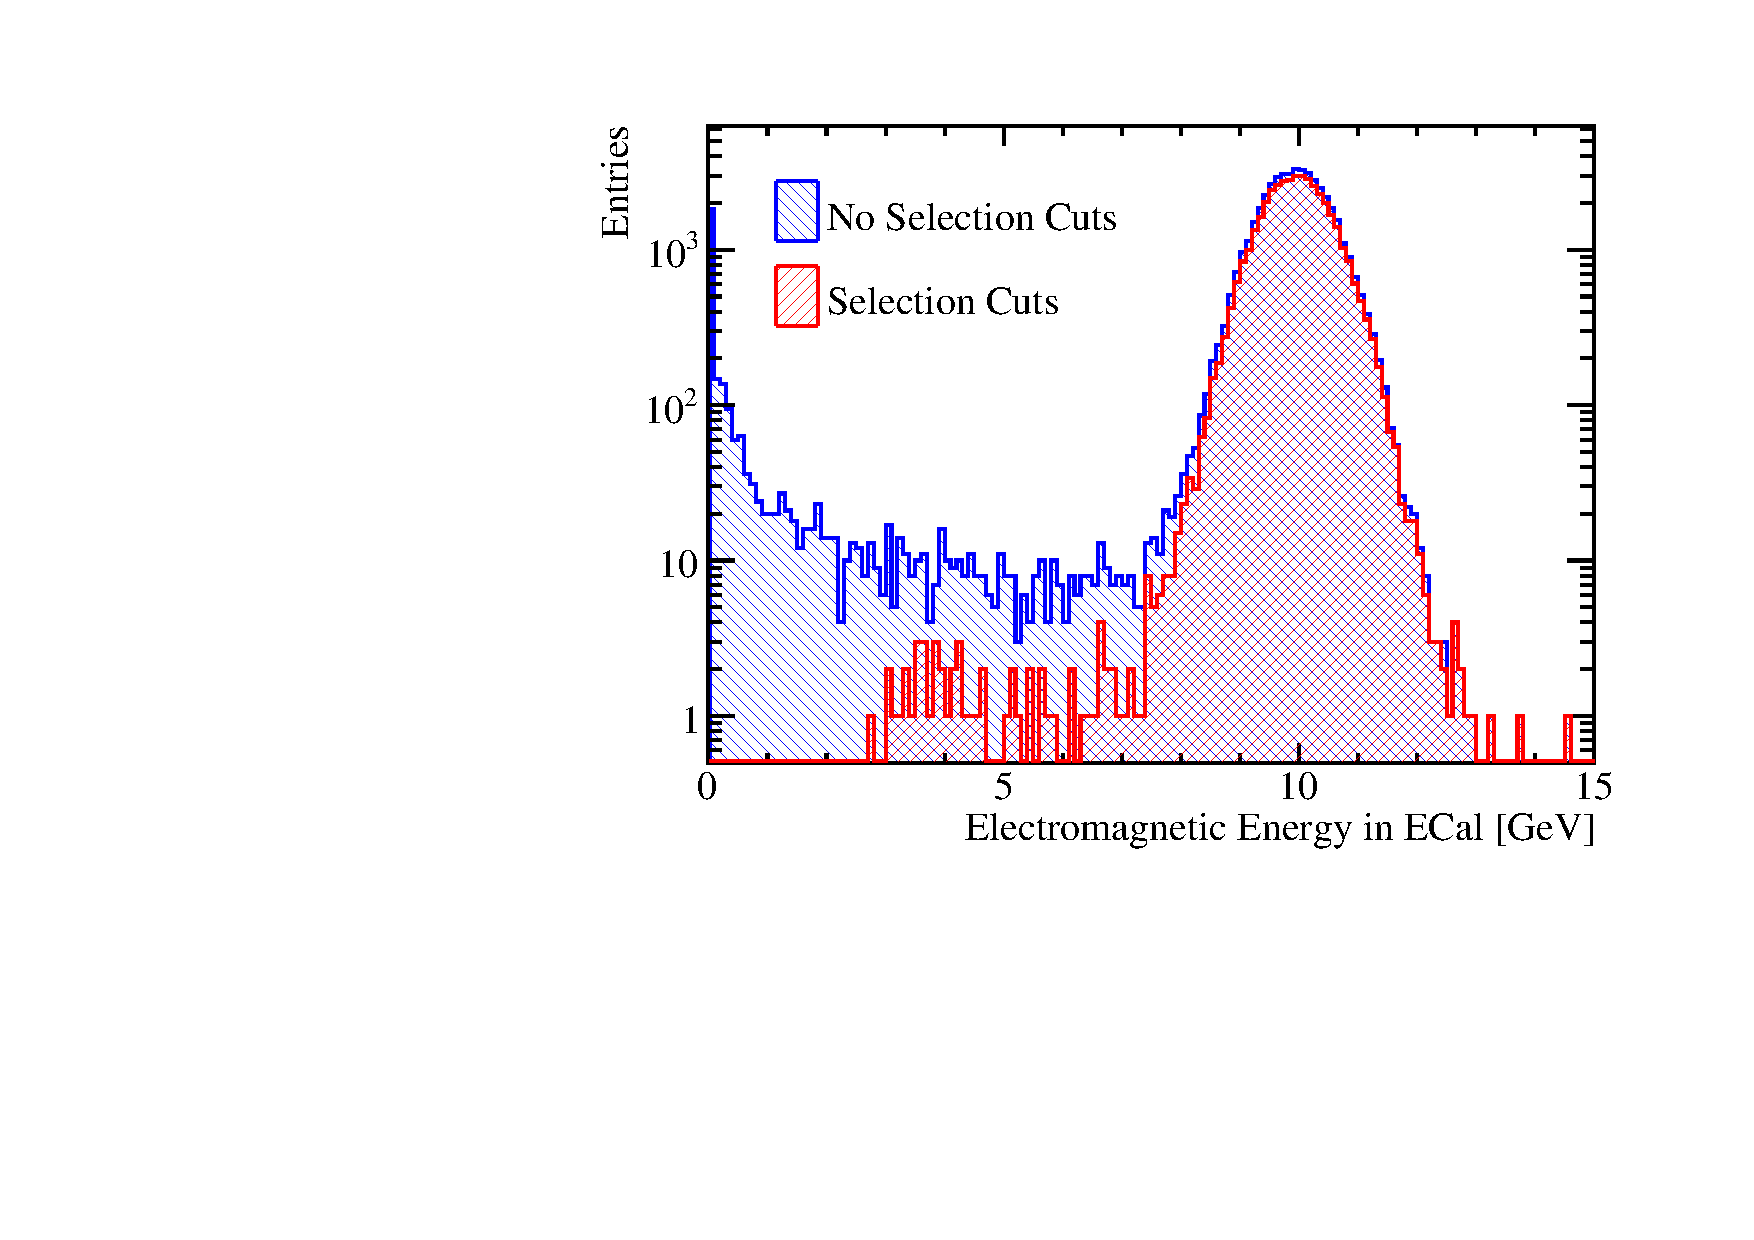
\includegraphics[width=0.5\textwidth]{EnergyEstimators/Plots/Calibration/EMScaleSetting/EMScaleECalSelection.pdf}}
\subfloat[]{\label{fig:ecalemscalefit}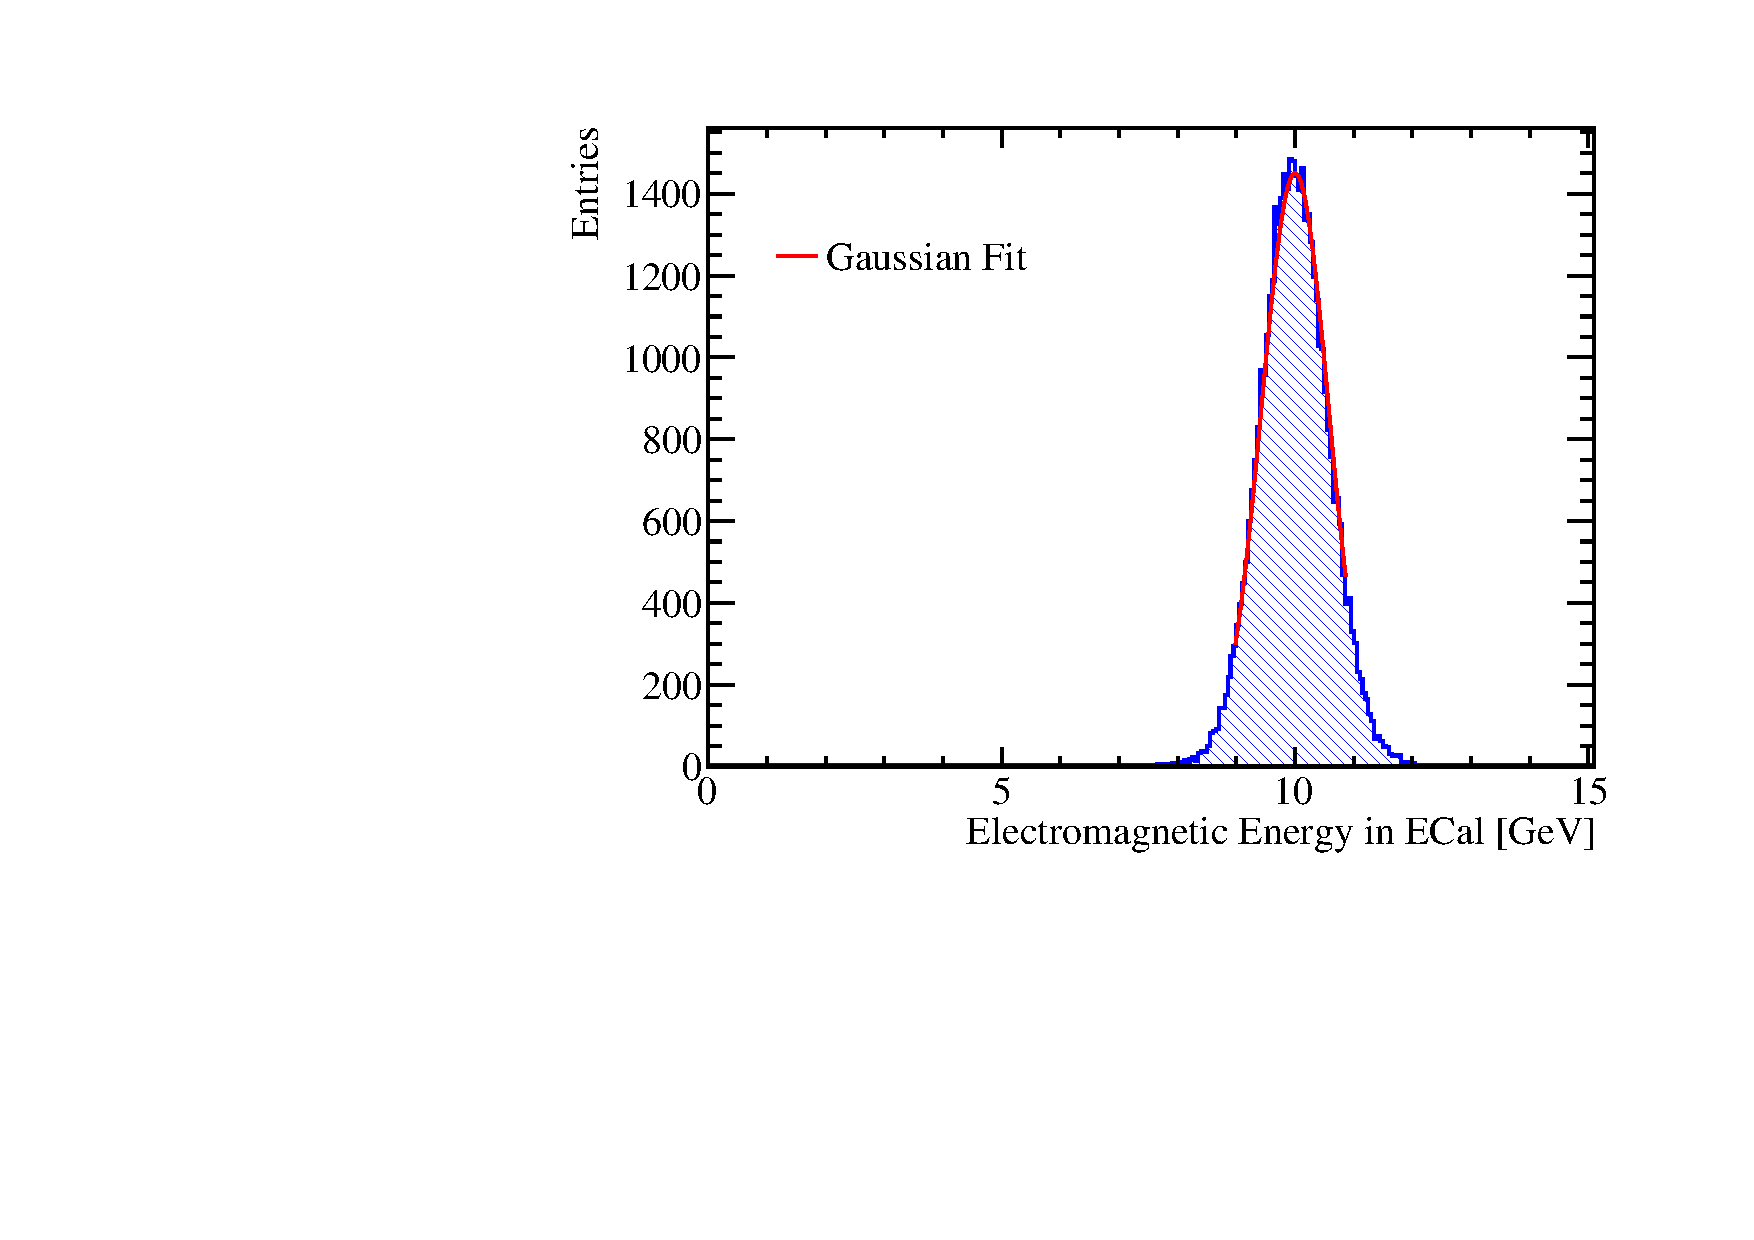
\includegraphics[width=0.5\textwidth]{EnergyEstimators/Plots/Calibration/EMScaleSetting/EMScaleSettingECalFit.pdf}}
\caption[\protect\subref{fig:ecalemscaleselection} The sum of the electromagnetic energy measured in the ECal for simulated 10~GeV photons with and without the selection cuts.  \protect\subref{fig:ecalemscalefit} Gaussian fit to sum of the electromagnetic energy deposited in the ECal for simulated 10~GeV photons with selection cuts.]{\protect\subref{fig:ecalemscaleselection} The sum of the electromagnetic energy measured in the ECal for simulated 10~GeV photons with and without the selection cuts.  \protect\subref{fig:ecalemscalefit} Gaussian fit to sum of the electromagnetic energy deposited in the ECal for simulated 10~GeV photons with selection cuts.}
\label{fig:ecalemscale}
\end{figure}

%========================================================================================

\subsection{Hadronic Scale in PandoraPFA}
\label{sec:hadscalesetting}
The hadronic energy scale factors for the ECal, $\beta^{Had}_{ECal}$, and HCal, $\beta^{Had}_{HCal}$, are determined using simulated $K^{0}_{L}$ events at $E_{MC} = 20$~GeV.  As the ECal contains approximately one nuclear interaction length, a non-negligible amount of hadronic energy will be deposited in the ECal, which makes the hadronic scale in the ECal, $\beta^{Had}_{ECal}$, important for detector performance.  The hadronic scale in the ECal and HCal are simultaneously set as it is unfeasible to create a large sample of 20~GeV $K^{0}_{L}$s that are fully contained within the ECal.

For the reasons outlined in section \ref{sec:hcaldigi}, the target reconstructed energy for the sample of $K^{0}_{L}$s used for setting the hadronic energy scale is the kinetic energy, $E_{K}$, as opposed to the total energy.  To ensure the events used are not affected by leakage of energy out of the back of the HCal, a cut is applied that vetoes events where energy is deposited in the outermost 10\% of the HCal.  In addition, a cut requiring a single neutral hadron to be reconstructed is applied to veto events with reconstruction failures and decays in the tracker.  Finally, it is required that the total hadronic energy measured within the calorimeters falls within three $\sigma$ of the kinetic energy of the $K^{0}_{L}$, where $\sigma$ is taken to be $55\% \times \sqrt{E_{K}}$~GeV.  This definition for $\sigma$ is approximately the energy resolution for neutral hadrons using the nominal ILD HCal \cite{Behnke:2013lya}.  This cut ensures that when fitting the two dimensional distribution of hadronic energy measured in the ECal and HCal, outliers do not skew the fit.   The impact of these selection cuts can be seen in figure \ref{fig:hadscaleselection}.

\begin{figure}[h!]
\subfloat[]{\label{fig:hadscaleselectionnocuts}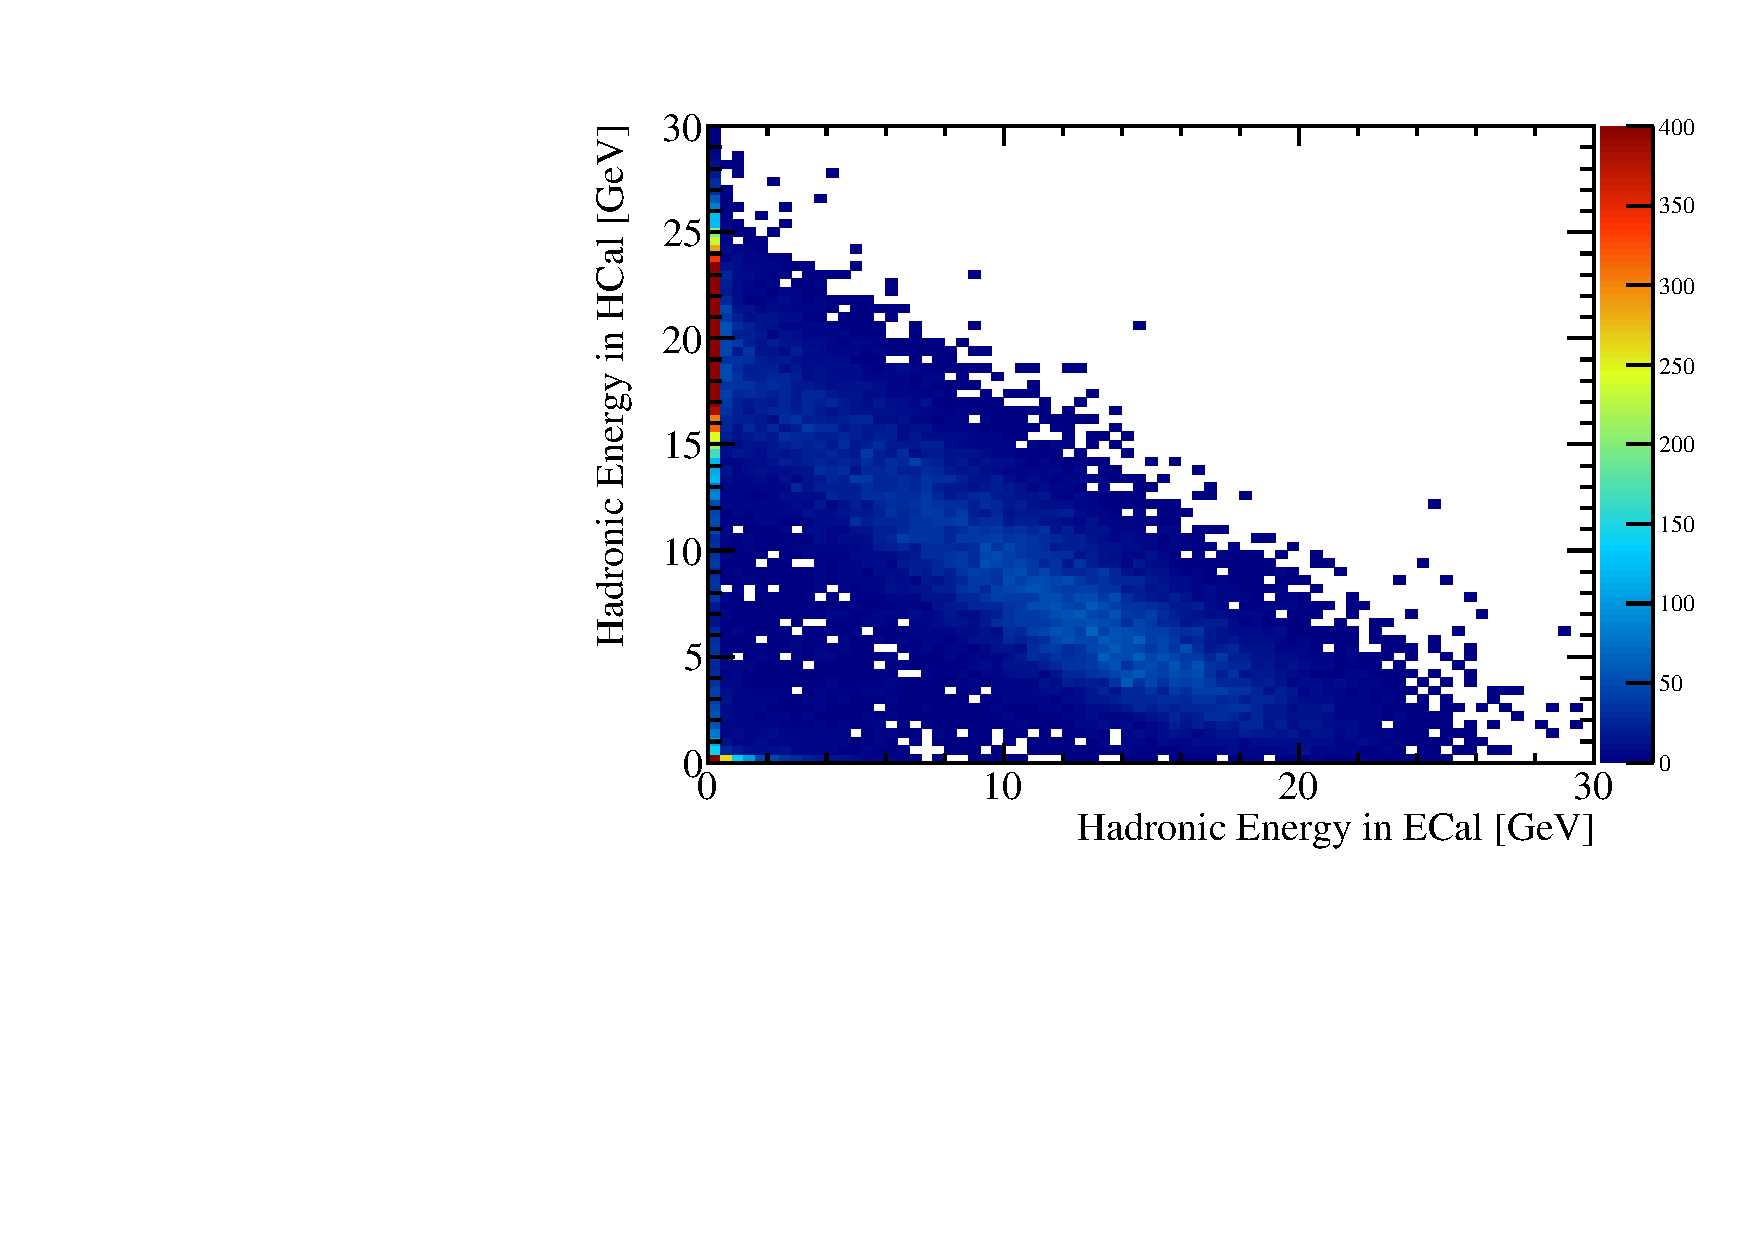
\includegraphics[width=0.5\textwidth]{EnergyEstimators/Plots/Calibration/HadScaleSetting/HadScaleECalHCalSelectionNoCuts.pdf}}
\subfloat[]{\label{fig:hadscaleselectioncuts}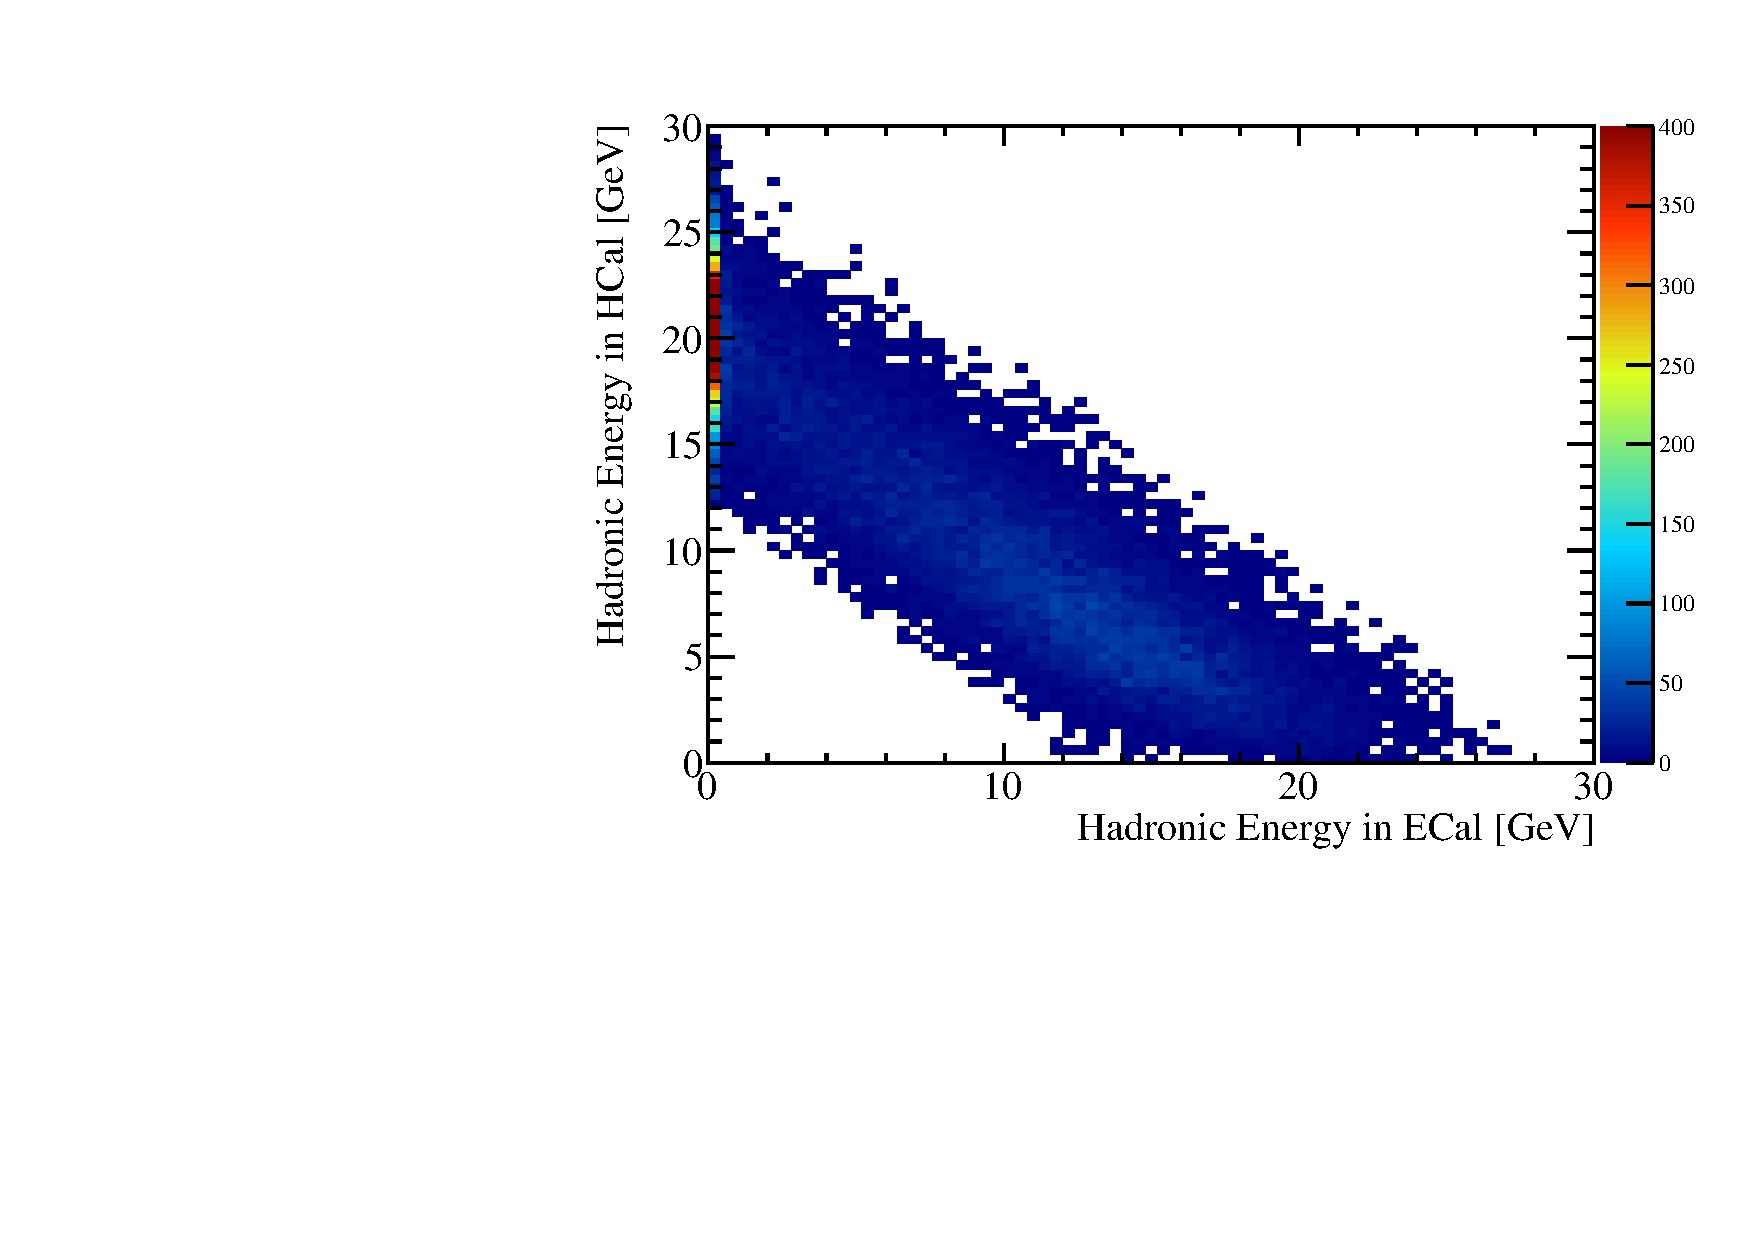
\includegraphics[width=0.5\textwidth]{EnergyEstimators/Plots/Calibration/HadScaleSetting/HadScaleECalHCalSelectionCuts.pdf}}
\caption[The distribution of hadronic energy measured in the ECal and HCal for 20~GeV $K^{0}_{L}$ events with and without selection cuts.]{The distribution of hadronic energy measured in the ECal and HCal for 20~GeV $K^{0}_{L}$ events \protect\subref{fig:hadscaleselectionnocuts} without selection cuts and \protect\subref{fig:hadscaleselectioncuts} with selection cuts.}
\label{fig:hadscaleselection}
\end{figure}

Determining the hadronic scale in PandoraPFA is an iterative process and begins by assuming trial values, $\beta^{Had0}_{ECal}$ and $\beta^{Had0}_{HCal}$, for the hadronic scale calibration factors $\beta^{Had}_{ECal}$ and $\beta^{Had}_{HCal}$.  The $K^{0}_{L}$ events are first reconstructed using the trial scale factors.  Then a linear fit is applied to the two dimensional distribution of the reconstructed hadronic energies measured in the ECal and HCal for events passing the selection cuts.  The best fit is obtained by minimising $\chi^{2}$ with respect to variables describing a linear fit to the distribution.  In this case, $\chi^{2}$ is defined as
%
\begin{equation}
\chi^{2}(\delta^{Had}_{ECal}, \delta^{Had}_{HCal}) = \sum_{i} \bigg( \frac{r_{i}}{\sigma_{r_{i}}} \bigg)^{2}\text{ ,}
\end{equation}
%
\noindent where $r_{i}$ is the perpendicular distance in the two dimensional plane of hadronic energies measured in the ECal and HCal from the point $(x_{i}, y_{i})$ to a straight line passing through the points $(\delta^{Had}_{ECal}, 0)$ and $(0, \delta^{Had}_{HCal})$.  In this definition, $x_{i}$ and $y_{i}$ are the hadronic energies measured in the ECal and HCal respectively for event $i$.  The variables $\delta^{Had}_{ECal}$ and $\delta^{Had}_{HCal}$ describe a linear fit to the hadronic energy distribution, which are to be varied when minimising $\chi^{2}$.  The explicit definition of $r_{i}$ is given in equation \ref{equ:xicalc} and illustrated in figure \ref{fig:hadscalechi2calc}.  The uncertainty on $r_{i}$ is given by $\sigma_{r_{i}}$, which is explicitly defined in equation \ref{equ:sigmaxicalc}.  This uncertainty is calculated by propagating the uncertainties on $x_{i}$ and $y_{i}$, which are assumed to be $\sigma_{x_{i}/y_{i}} = 55\% \times \sqrt{x_{i}/y_{i}}$, into the expression for $r_{i}$.  The sum runs over all events, $i$, passing the selection cuts.  
%
\begin{equation}
r_{i} = \frac{y_{i} \delta^{Had}_{ECal} + x_{i} \delta^{Had}_{HCal} - \delta^{Had}_{ECal} \delta^{Had}_{HCal}}{\sqrt{(\delta^{Had}_{ECal})^{2} + (\delta^{Had}_{HCal})^{2}}}\text{ ,}
\label{equ:xicalc}
\end{equation}
\begin{equation}
\sigma_{i} = \frac{(\sigma_{y_{i}}  \delta^{Had}_{ECal})^{2} + (\sigma_{x_{i}} \delta^{Had}_{HCal})^{2}}{\sqrt{(\delta^{Had}_{ECal})^{2} + (\delta^{Had}_{HCal})^{2}}}\text{ .}
\label{equ:sigmaxicalc}
\end{equation}
%
\begin{figure}[h!]
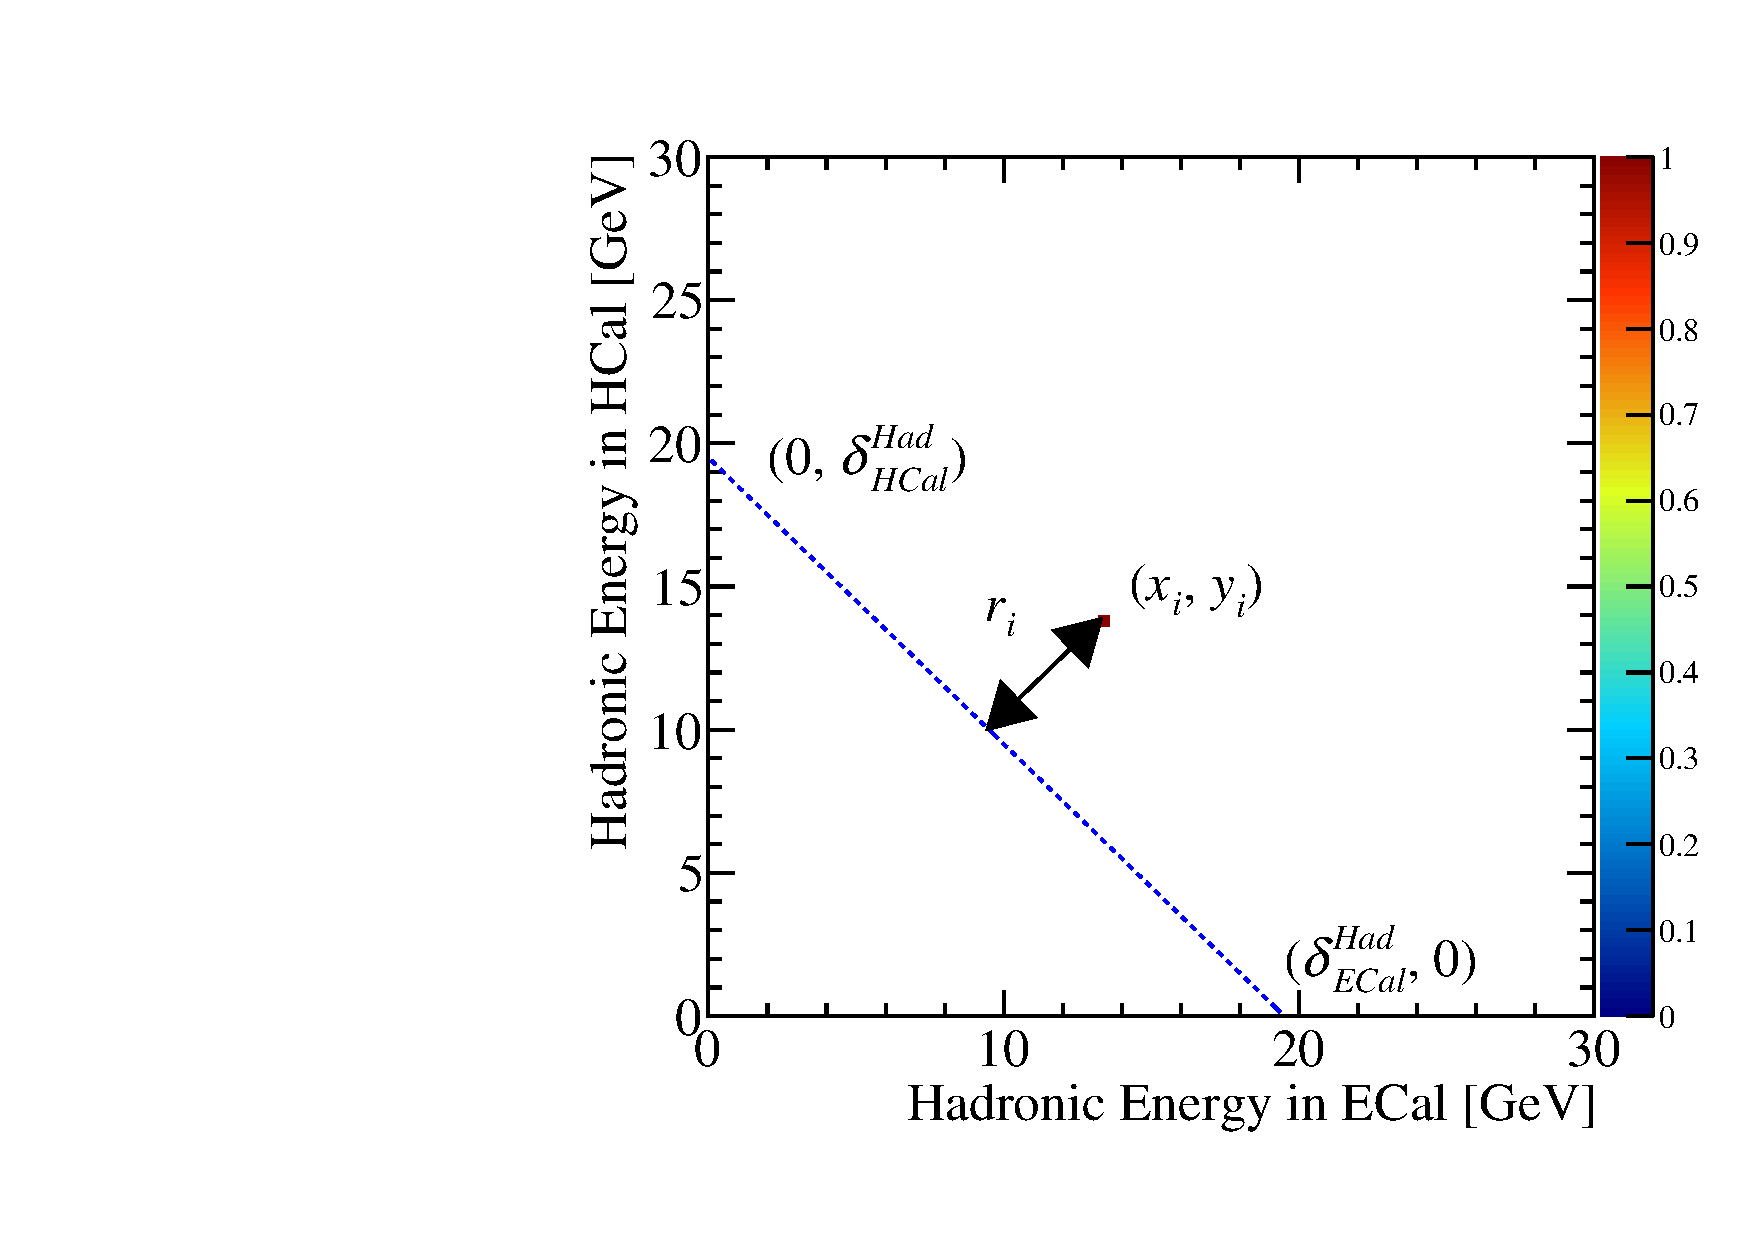
\includegraphics[width=0.5\textwidth]{EnergyEstimators/Plots/Calibration/HadScaleSetting/HadScaleECalHCalSelectionExample.pdf}
\caption[An example showing the definition of $r_{i}$.  The blue dotted line corresponds to $y_{i} = \delta^{Had}_{HCal} - x_{i} \delta^{Had}_{HCal} / \delta^{Had}_{ECal}$.]{An example showing the definition of $r_{i}$.  The blue dotted line corresponds to $y_{i} = \delta^{Had}_{HCal} - x_{i} \delta^{Had}_{HCal} / \delta^{Had}_{ECal}$.}
\label{fig:hadscalechi2calc}
\end{figure}
%
\noindent The minimisation of $\chi^{2}$ is done by stepping over a range of $\delta^{Had}_{ECal}$ and $\delta^{Had}_{HCal}$ centred about the ideal value of $E_{K}$ in search for the minimum $\chi^{2}$.  Once the minima in $\chi^{2}$ is found the trial calibration factors $\beta^{Had0}_{ECal}$ and $\beta^{Had0}_{ECal}$ are rescaled to correct for any deviation from the desired fit as follows
%
\begin{equation}
\beta^{Had0}_{ECal} \rightarrow \beta^{Had}_{ECal} = \beta^{Had0}_{ECal} \times \frac{E_{K}}{\Delta^{Had}_{ECal}} \text{ ,}\\
\beta^{Had0}_{HCal} \rightarrow \beta^{Had}_{HCal} = \beta^{Had0}_{HCal} \times \frac{E_{K}}{\Delta^{Had}_{HCal}}\text{ ,}
\end{equation}
%
\noindent where $\Delta^{Had}_{ECal}$ and $\Delta^{Had}_{ECal}$ are the values of $\delta^{Had}_{ECal}$ and $\delta^{Had}_{ECal}$ giving the minimum $\chi^{2}$.  The step size used for minimising $\chi^{2}$ with respect to $\delta^{Had}_{ECal}$ and $\delta^{Had}_{ECal}$ was chosen such that a single step would correspond to the final tolerance on $\delta^{Had}$, which in this case is $\approx$ 0.1~GeV.  This procedure is then repeated using the updated hadronic scaling factors until $\Delta^{Had}_{ECal}$ and $\Delta^{Had}_{ECal}$ both fall within a specified final tolerance, which in this case is taken to be $|\Delta^{Had}_{E/HCal} - E_{\text{{K}}}| < E_{\text{{K}}} \times 0.5 \% \approx 0.1$~GeV.

The electromagnetic scale in the HCal, $\beta^{EM}_{HCal}$, is chosen to be equal to the hadronic scale in the HCal, $\beta^{Had}_{HCal}$.  For the ILC and CLIC, $\beta^{EM}_{HCal}$ is not a critical parameter in the reconstruction as photons are largely contained within the ECal meaning little to no electromagnetic energy is measured in the HCal.  

Setting the hadronic scale in PandoraPFA ensures that the energy estimators for neutral hadrons are accurate at 20~GeV, however, this is not true for all energies.  The undetectable energy component of a hadronic shower varies as a function of particle shower energy \cite{Wigmans:2000vf}, which means the response of a calorimeter to neutral hadrons non-linear with the hadron energy.  This is an inherent limitation of this calibration procedure that will be addressed by the development of more sophisticated energy estimators in subsequent chapters.  

%========================================================================================
%========================================================================================

\subsection{Summary}
The procedure for setting the MC response in the linear collider detector simulation has been outlined.  This procedure ensures that when modifying the detector simulation, the response of the detector will yield reliable energy estimators for particles showering in the calorimeter.  For completion, after this calibration procedure has been applied, retraining of the likelihood data used by specific algorithms in PandoraPFA for the reconstruction of photons can be performed.  

%========================================================================================
%========================================================================================

\section{Novel Energy Estimators}
This section describes two novel energy estimators that are introduced with a view to improving the energy resolution for hadronic showers.  Two techniques will be discussed: HCal hit energy truncation, which focuses on limiting the impact of Landau fluctuations; and software compensation, which focuses on obtaining a compensating calorimeter response.  Both of these techniques are implemented by introducing weights, $\omega^{i}$, to calorimetric energy deposits made by showering particles in the HCal.  The energy of a showering particle, $E_{Cluster}$, is determined by grouping together a clusters of calorimeter hits and summing their energies.  When weights are applied to HCal hits this energy estimator becomes 
%
\begin{equation}
E_{Cluster} & = \sum_{ECal \text{ } hits \text{, }i} E^{i}_{ECal} +\sum_{HCal \text{ } hits \text{, }i} E^{i}_{HCal} \omega^{i}(\rho^{i}) \text{ .}
\label{equ:compensation}
\end{equation}
%
\noindent Weights are only applied to calorimeter hits in the HCal as these techniques modify the energy of hadronic showers, which are primarily contained within the HCal.  The weights, $\omega^{i}$, vary a function of the energy density of the calorimeter hit, $\rho^{i} = E^{i}_{HCal}/V$ where $V$ is the physical volume of a calorimeter hit in the HCal, which includes the both the active and absorber layer thicknesses.  

Although the exact weights depend on the implementation of the technique, a general feature is that at large $E^{i}_{HCal}$ the weight is less than one.  This limits the impact of spuriously high energy hits caused by Landau fluctuations.  The energy loss probability distribution function for scintillator detectors, such as the ILD HCal, is given by a Landau function \cite{Landau:1944if}.  Energy deposits from the high energy tail of this distribution, which are known as Landau fluctuations, account for high energy knock-on electrons that appear within particle showers \cite{Bichsel:2004ej}.  As Landau fluctuations deposit a disproportionately large amount of energy with respect to the bulk of the particle shower, they can lead to overestimates of the particle shower energy.  

The energy loss probability distribution function for $n$ particles passing through a calorimeter hit is given by the convolution of $n$ Landau functions, which by the central limits theorem will tend to a Gaussian as $n$ becomes large.  Consequently, as the average number of particles passing through a calorimeter hit increases, the high energy tail in the energy loss probability distribution function for the hit becomes less pronounced and the impact of Landau fluctuations decreases.  This means that the impact of Landau fluctuations on energy measurements is dictated by the density of a particles within a particle shower and the transverse segmentation, or cell size, of the calorimeter in use.  If the transverse segmentation, or cell size, of a calorimeter decreases, the average number of particles passing through each hit decreases and the impact of Landau fluctuations increases.  Any technique used for minimising the impact of Landau fluctuations will be sensitive to the transverse segmentation of the calorimeters in use.  

%========================================================================================

\subsection{HCal Hit Energy Truncation}
\label{sec:hcalcelltruncation}
The first technique to be examined is a simple truncation of the hadronic energy, $E$, recorded in any given HCal hit
%
\begin{equation}
E \rightarrow E' =
\begin{cases}
E & \text{if } E < \kappa \text{ ,} \\
\kappa & \text{otherwise} \text{ ,}
\end{cases}
\end{equation}
%
\noindent where $\kappa$ is the value of the truncation.  This improves the energy estimators for hadronic clusters by limiting the impact of Landau fluctuations.  In terms of $\omega$ introduced in equation \ref{equ:compensation} the truncation corresponds to
%
\begin{equation}
\omega(\rho) =
\begin{cases}
1 & \text{if } \rho \times V < \kappa \text{ ,} \\
\frac{\kappa}{\rho \times V} & \text{otherwise} \text{ .}
\end{cases}
\end{equation}
%
\noindent This weight as a function of hit energy density is shown in figure \ref{fig:hcalcellweight}.  

\begin{figure}[h!]
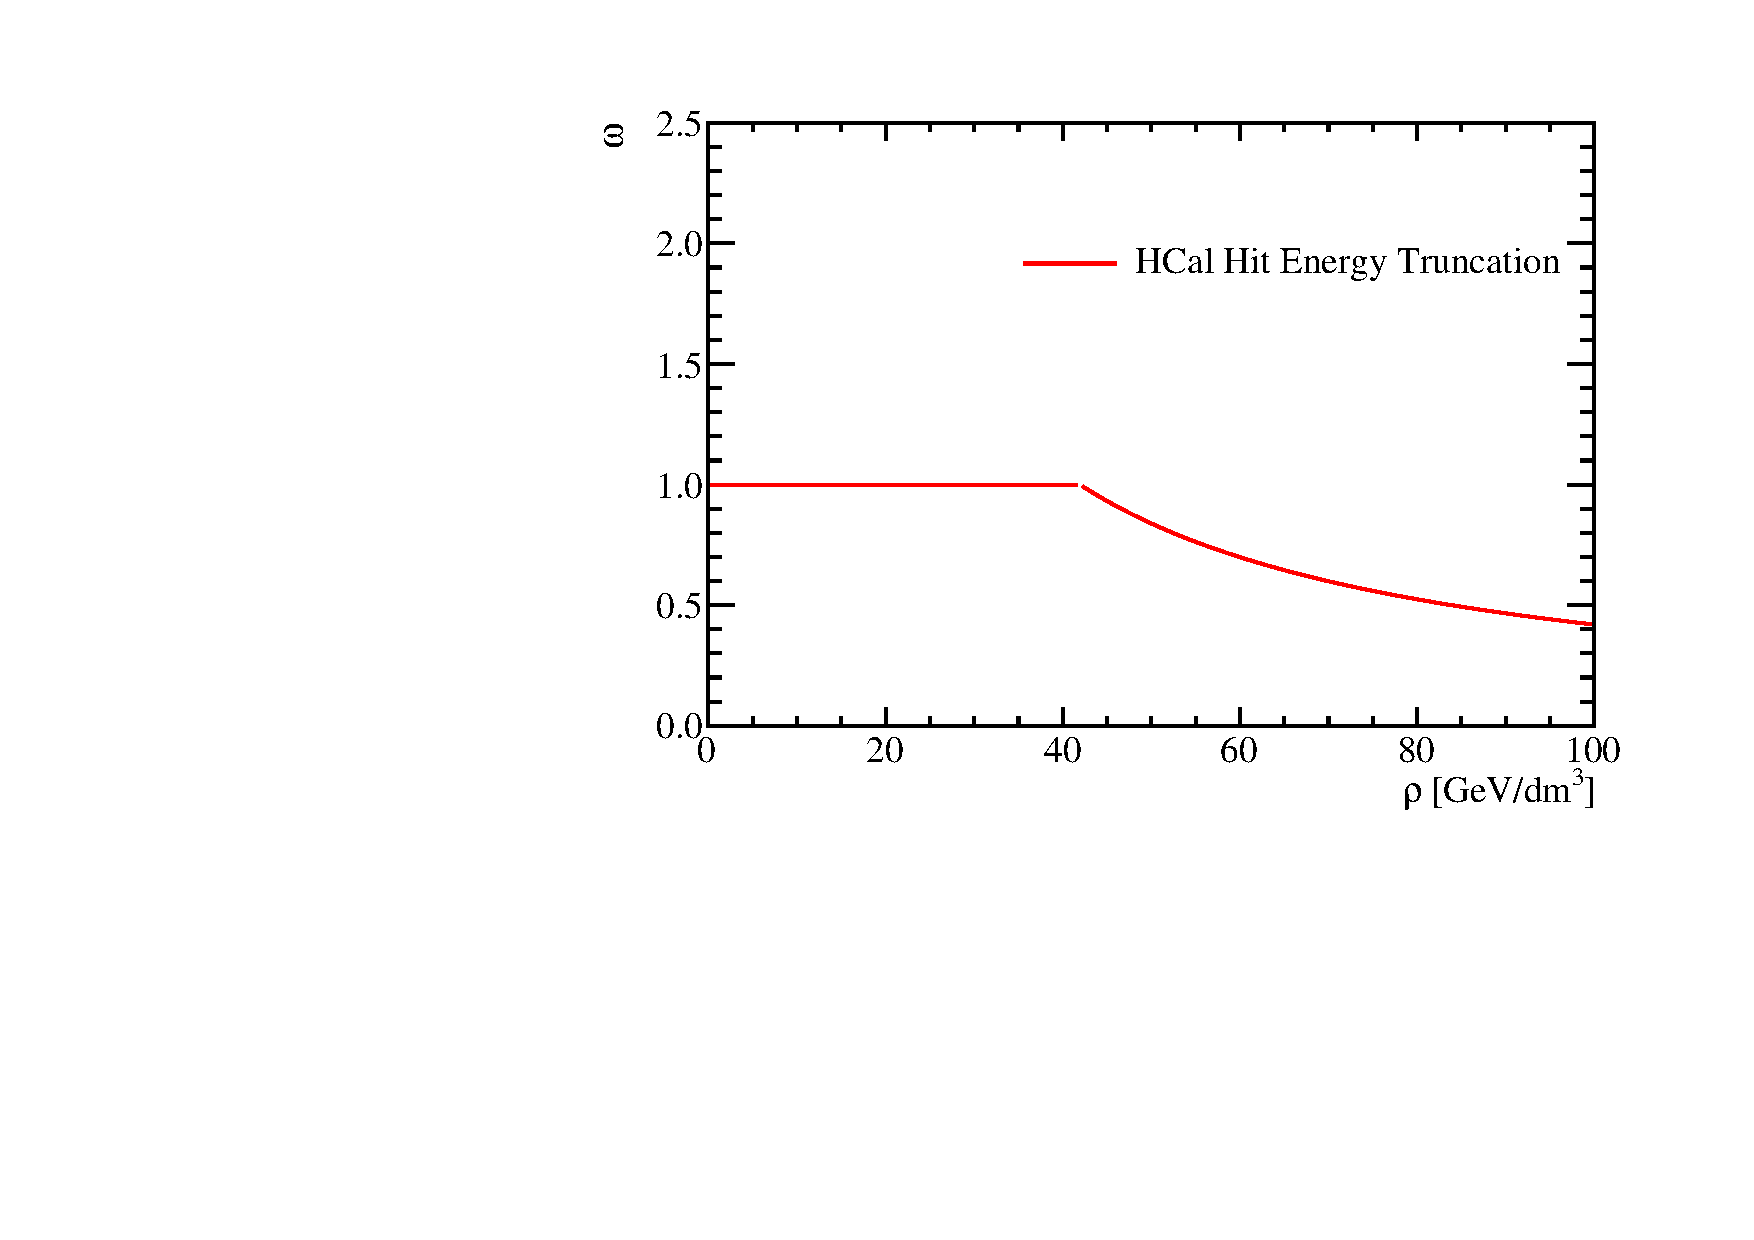
\includegraphics[width=0.5\textwidth]{EnergyEstimators/Plots/SoftComp/Weights/CellTruncWeights.pdf}
\caption[The weights, $\omega$, used in the HCal hit energy truncation as a function of the energy density of the HCal hit, $\rho$.  The truncation shown here corresponds to a 1~GeV truncation in the nominal ILD HCal.]{The weights, $\omega$, used in the HCal hit energy truncation as a function of the energy density of the HCal hit, $\rho$.  The truncation shown here corresponds to a 1~GeV truncation in the nominal ILD HCal.}
\label{fig:hcalcellweight}
\end{figure}

%========================================================================================

\subsubsection{Legacy Energy Corrections}
\label{sec:legacycorrections}
Alongside the HCal hit energy truncation, PandoraPFA also applied two other energy corrections designed at limiting the impact of Landau fluctuations.  They are:

\begin{itemize}
\item \textbf{Clean Clusters}.  This algorithm checks to see whether the energy measured within a calorimeter hit is anomalously high.  Anomalously high energy hits are defined as hits where the energy contained within the hit is greater than 10\% of the energy of the cluster that the hit has been associated to.  If a hit is deemed to have an anomalously high energy and if this energy is above a threshold (0.5~GeV) the hit energy used by PandoraPFA is modified.  The updated hit energy is taken as the average hit energy in the calorimeter layers immediately before and after the layer containing the high energy hit.    
\item \textbf{Scale Hot Hadrons}.  This algorithm calculates the average energy of the calorimeter hits in a given cluster cluster in units of, normally incident, MIP equivalent particles.  If this number is larger than a certain value, default 15 MIPs per hit, the cluster energy is rescaled to give a lower average number of MIPs per hit, default is 5 MIPs per hit.  
\end{itemize}

In the reconstruction, these corrections are applied to each cluster of calorimeter hits, irrespective of the location of that cluster in the detector.  These algorithms, with the HCal hit truncation, form the "legacy" energy corrections that are used by PandoraPFA when performing the event reconstruction.    

%========================================================================================

\subsubsection{Impact on Single Particle Energy Resolution}
Figure \ref{fig:ercelltrunckaons} shows the energy resolution for neutral hadrons as a function of the HCal hit energy truncation.  The optimal truncation for the ILD detector model simulation was 1~GeV and, using this truncation, a neutral hadron energy resolution of $\sim 8.8\% = 62\% / \sqrt{E\text{(GeV)}}$ was obtained for $E = 50~GeV$ $K^{0}_{L}$ events.  In comparison, the neutral hadron energy resolution for $E = 50~GeV$ $K^{0}_{L}$ events obtained without a truncation was $\sim 10.4\% = 74\% / \sqrt{E\text{(GeV)}}$.  Smaller energy truncations begin to truncate the energy of calorimeter hits produced in typical hadronic shower development, while larger truncations allow for a larger impact from Landau fluctuations.  Both of these effects result in worsening neutral hadron energy resolutions.  For completeness the photon energy resolutions as a function of HCal hit energy truncation are shown in figure \ref{fig:ercelltruncphotons}.  As expected the photon energy resolution is unaffected by the HCal hit energy truncation as the photons are largely contained within the ECal.

\begin{figure}[h!]
\subfloat[]{\label{fig:ercelltrunckaons}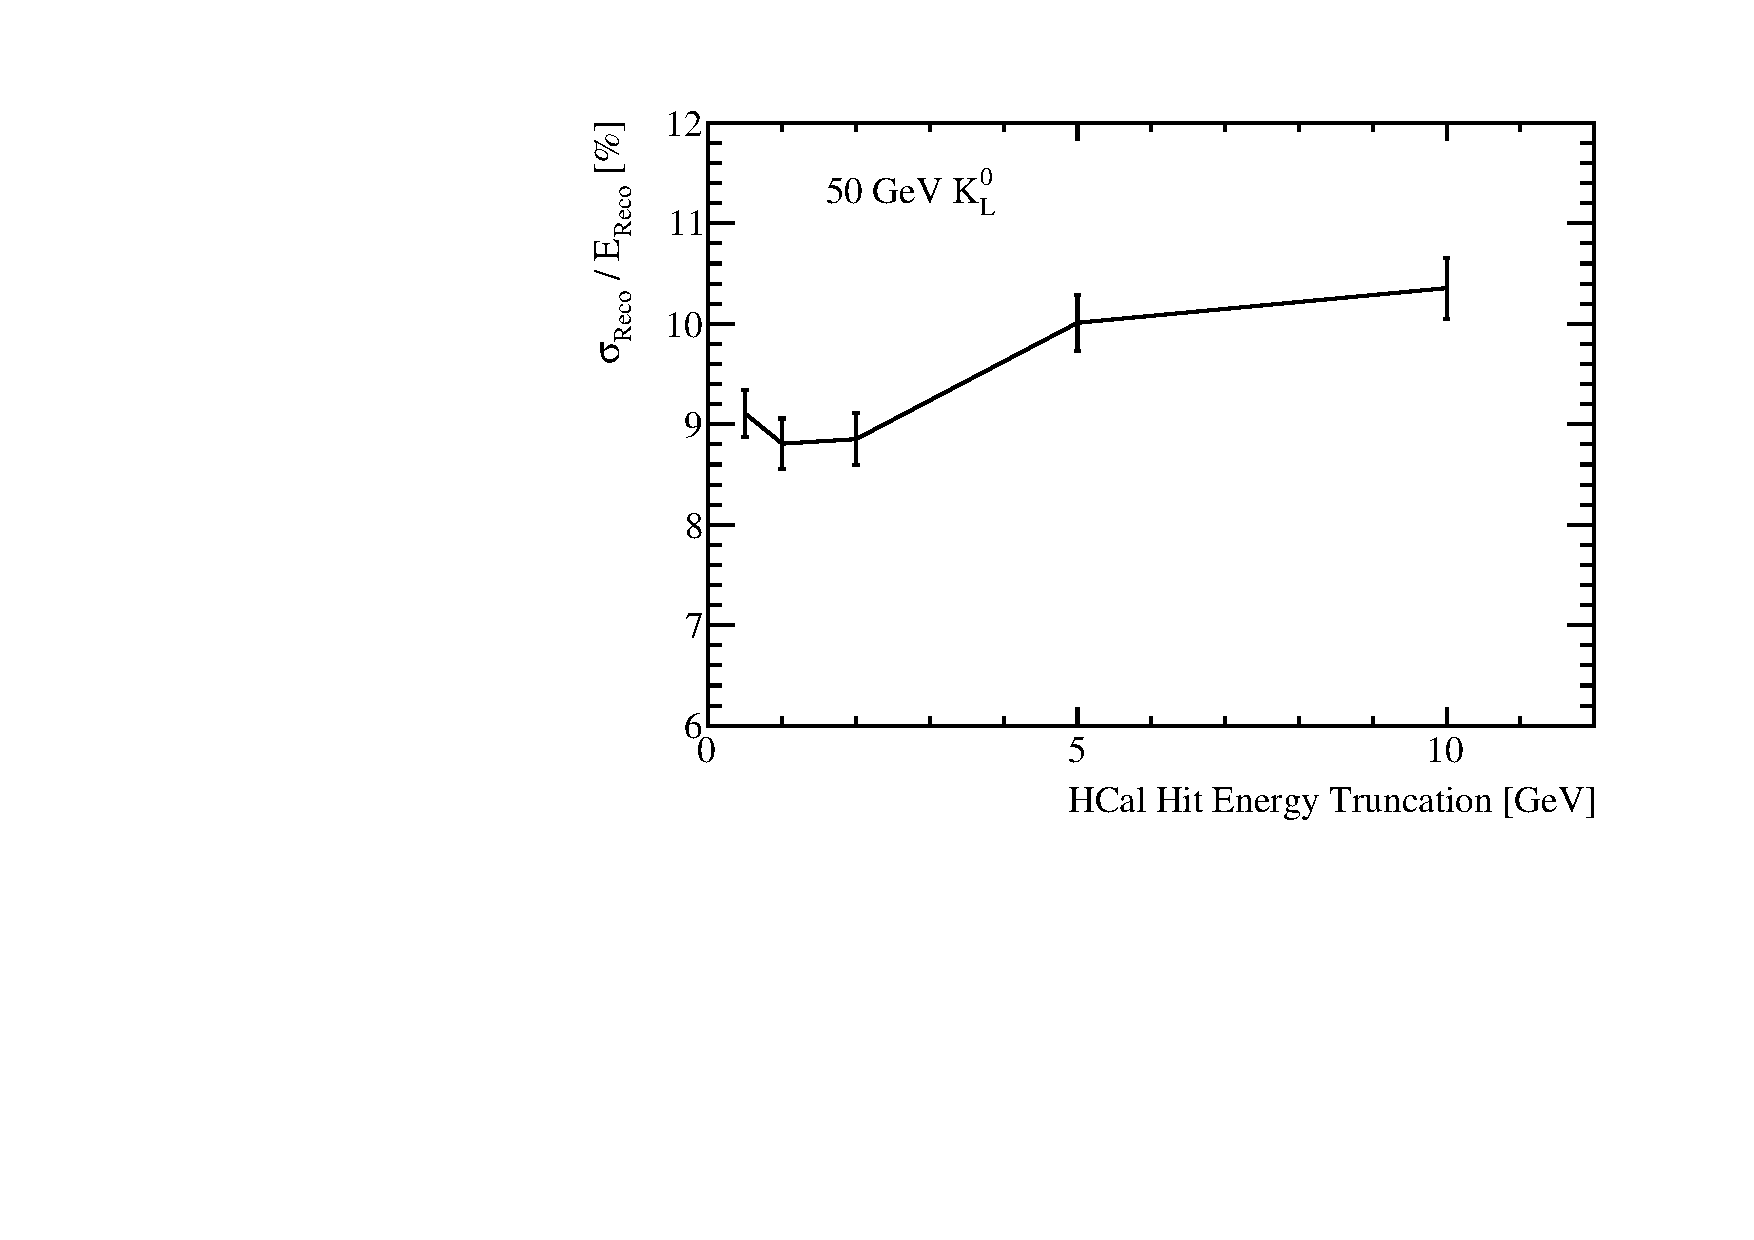
\includegraphics[width=0.5\textwidth]{EnergyEstimators/Plots/CellTruncation/ER_vs_Kaon0LCellTrunc_50GeVKaon0L.pdf}}
\subfloat[]{\label{fig:ercelltruncphotons}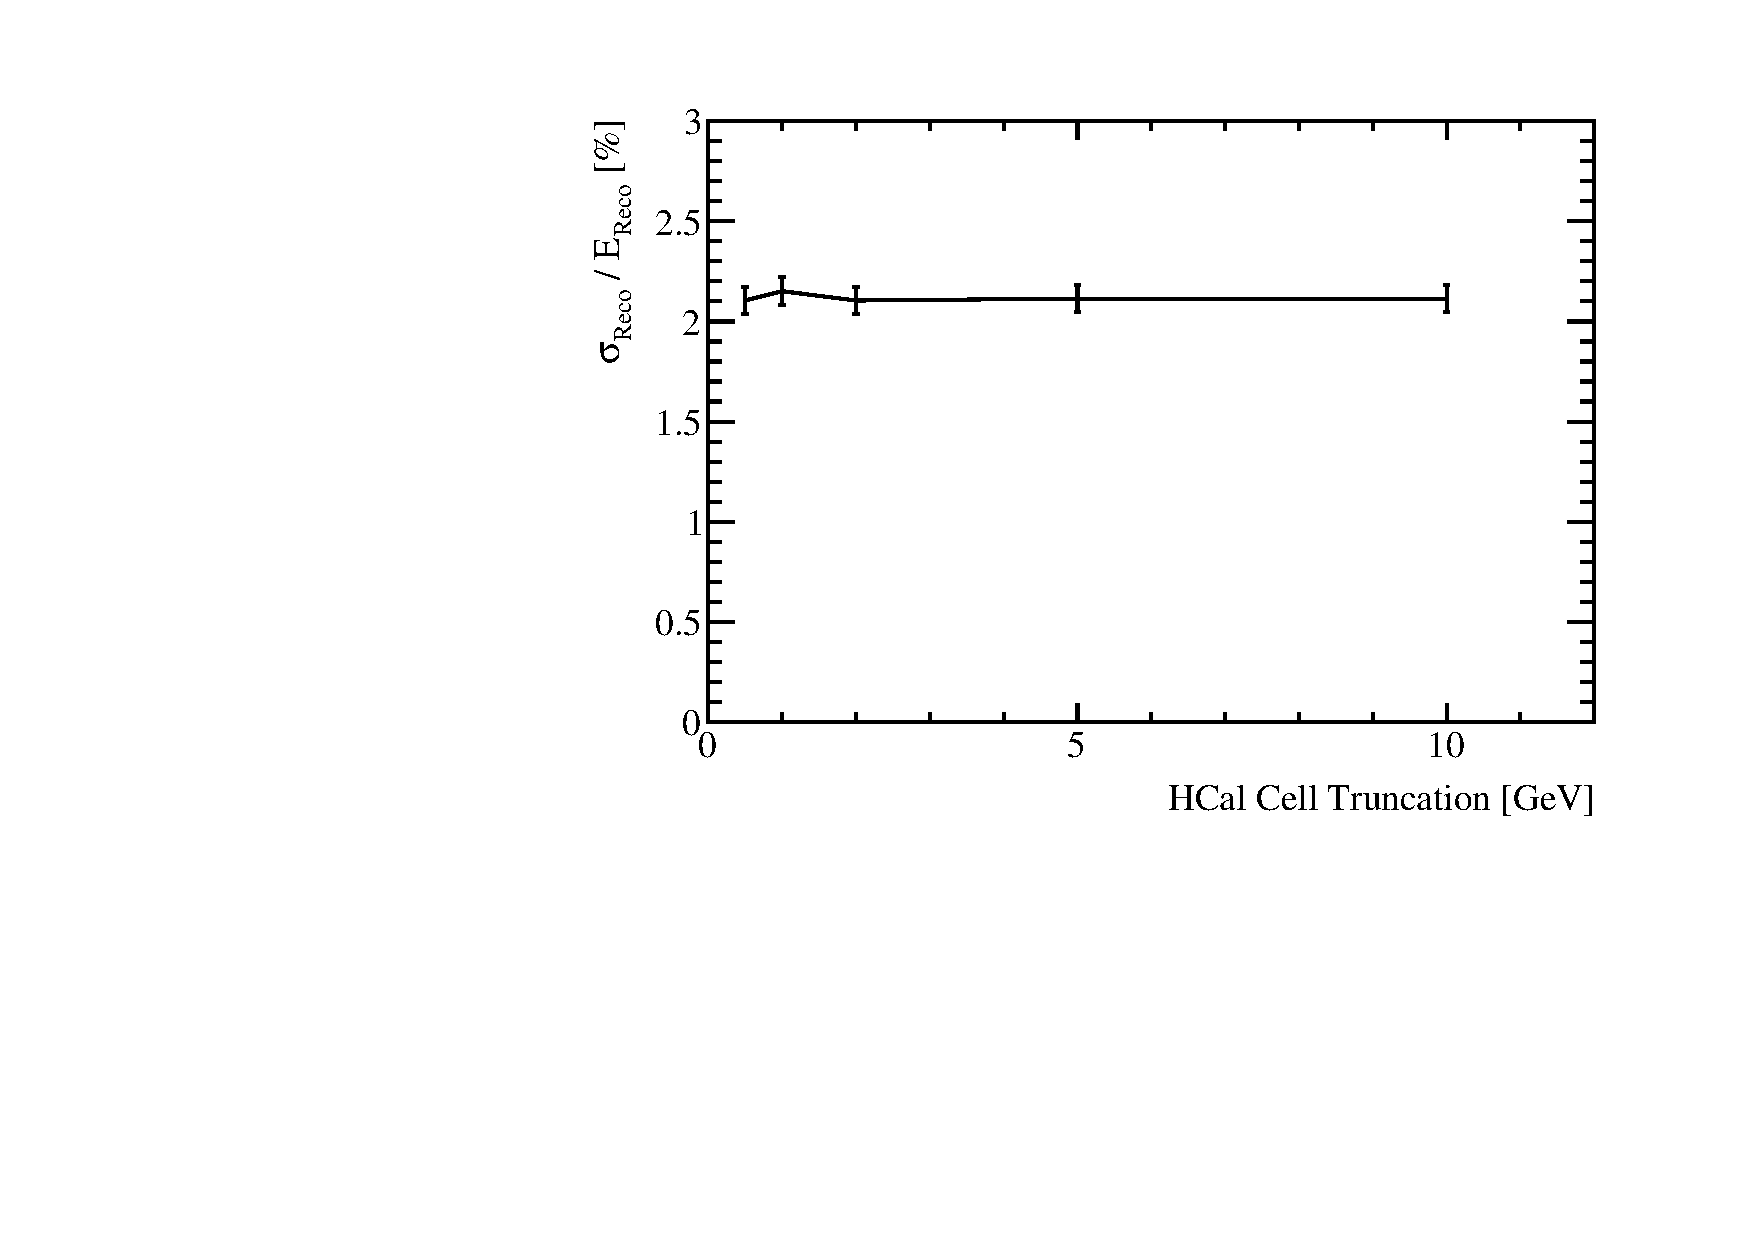
\includegraphics[width=0.5\textwidth]{EnergyEstimators/Plots/CellTruncation/ER_vs_PhotonCellTrunc_100GeVPhoton.pdf}}
\caption[The energy resolution as a function of HCal cell truncation for \protect\subref{fig:ercelltrunckaons} 50~GeV $K^{0}_{L}$ events and \protect\subref{fig:ercelltruncphotons} 100~GeV photons using the nominal ILD detector model.]{The energy resolution as a function of HCal cell truncation for \protect\subref{fig:ercelltrunckaons} 50~GeV $K^{0}_{L}$ events and \protect\subref{fig:ercelltruncphotons} 100~GeV photons using the nominal ILD detector model.}
\label{fig:ercelltrunc}
\end{figure}

%========================================================================================

\subsubsection{Impact on Jet Energy Resolution}
Figure \ref{fig:jercelltrunc} shows the jet energy resolution as a function of jet energy for selected values of the HCal hit energy truncation.  The trends in this plot are complex as the optimal HCal hit energy truncation varies with the jet energy.  For 45.5~GeV jets, the best jet energy resolution, $\sim$3.6\%, is obtained using a 0.5~GeV truncation, while for 180~GeV jets, the best jet energy resolution, $\sim$2.9\%, is obtained using a 1~GeV truncation.  This is expected because at low jet energies the average number of particles passing through each active calorimeter hit will be small, meaning the impact of Landau fluctuations is large and that to limit them a low truncation energy is needed.  As the jet energy increases more particles on average pass through each calorimeter hit and the impact of Landau fluctuations decreases.  

\begin{figure}[h!]
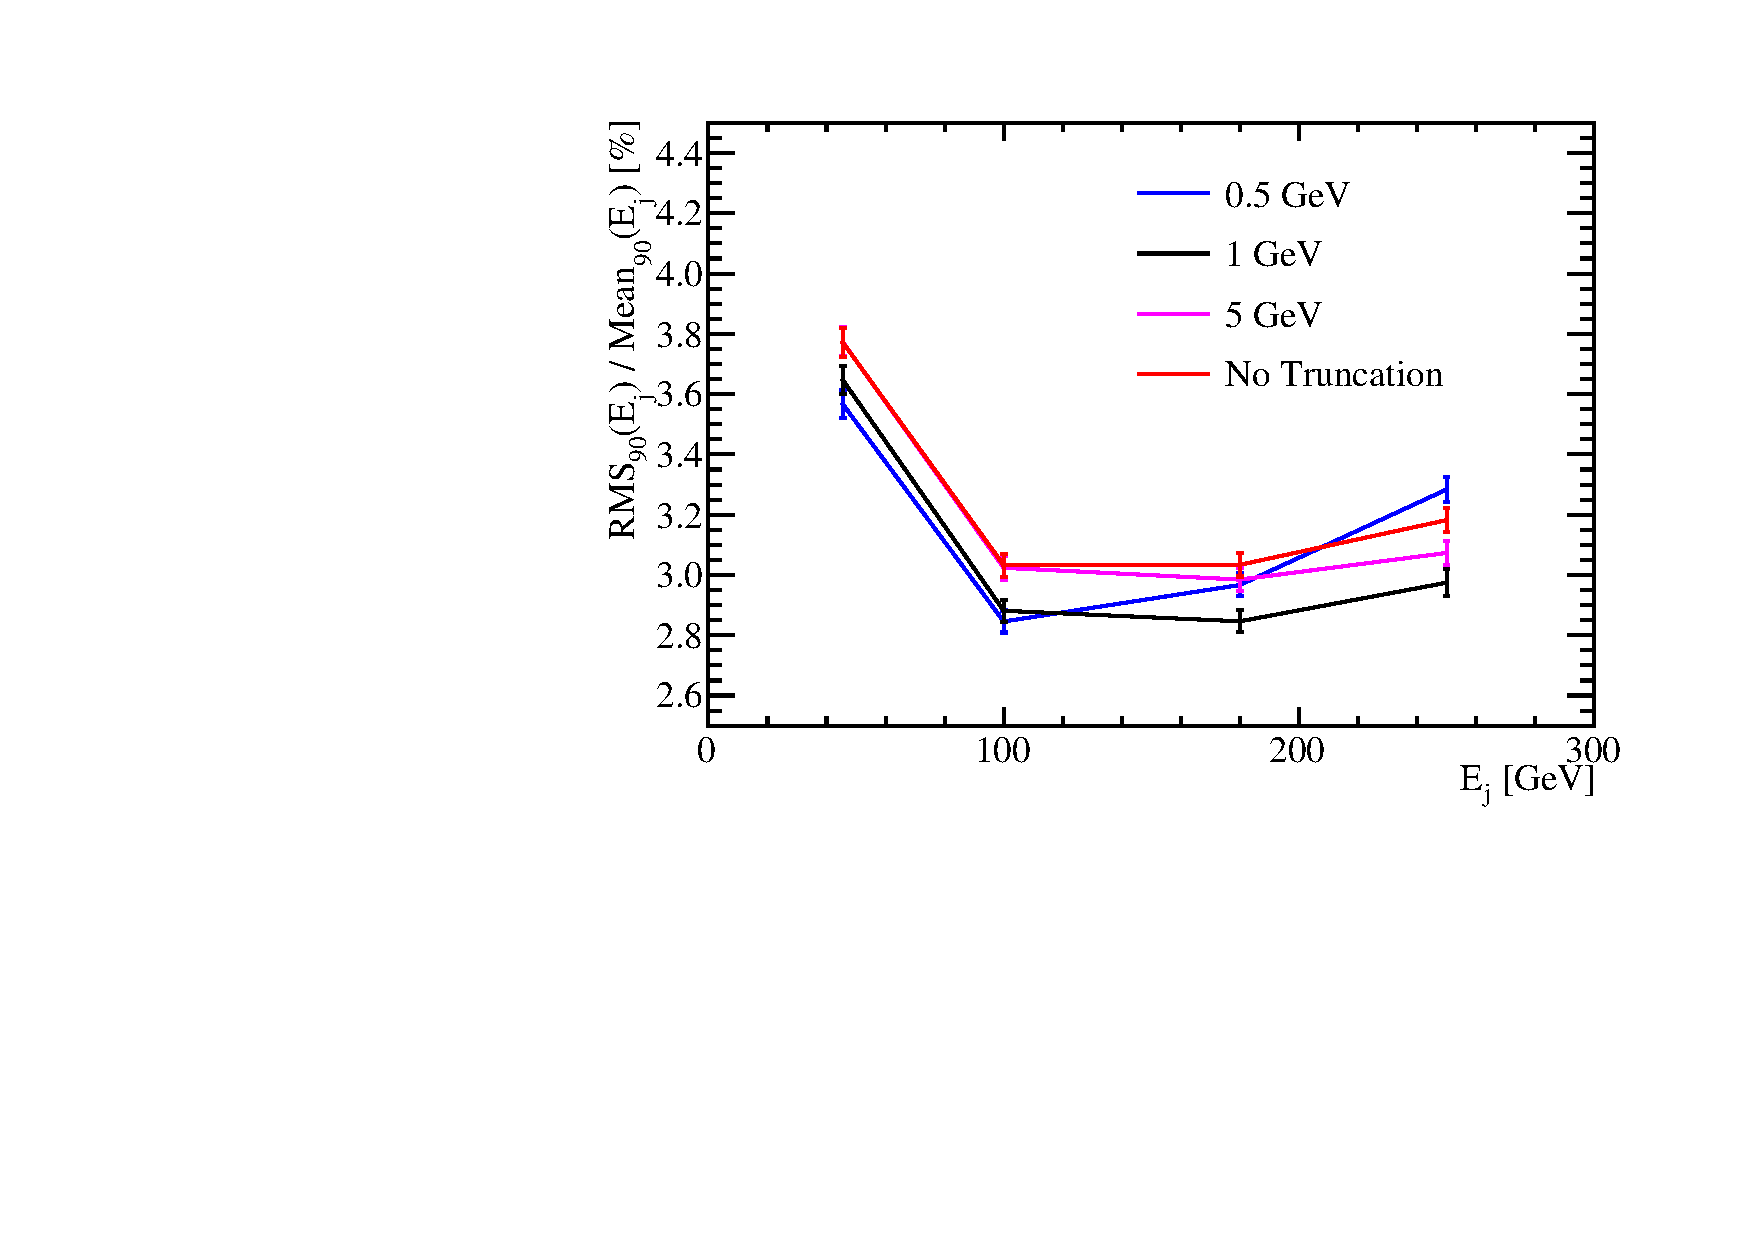
\includegraphics[width=0.5\textwidth]{EnergyEstimators/Plots/CellTruncation/JER_vs_JetEnergy_HCalCellTruncation.pdf}
\caption[The jet energy resolution as a function of jet energy for various HCal hit energy truncations.  The results shown use the nominal ILD detector model, which contains $30\times30 \text{ mm}^{2}$ square scintillator tiles in the HCal.]{The jet energy resolution as a function of jet energy for various HCal hit energy truncations.  The results shown use the nominal ILD detector model, which contains $30\times30 \text{ mm}^{2}$ square scintillator tiles in the HCal.}
\label{fig:jercelltrunc}
\end{figure}

It is clear that a 1~GeV HCal hit energy truncation is beneficial for the performance of the nominal ILD detector model since the jet energy resolution is reduced by roughly $\sim$0.15\% across the jet energy range from 45.5~GeV to 250~GeV.  As the HCal hit truncation technique offers significant performance gains, it is used for the calorimeter optimisation studies presented in chapter \ref{chap:detopt}.  These studies include optimisation of the HCal cell size.  Increasing the HCal cell size will increase the average number of particles passing through each calorimeter hit, which in turn reduces the impact of Landau fluctuations and vice verse.  For all detector models considered where the HCal cell size was varied, the HCal hit energy truncation was reoptimsied to account for the changing impact of Landau fluctuations.  For detector models with a HCal cell size of $10 \times 10\text{ mm}^{2}$, $20 \times 20\text{ mm}^{2}$, $30 \times 30\text{ mm}^{2}$, $40 \times 40\text{ mm}^{2}$, $50 \times 50\text{ mm}^{2}$ and $100 \times 100\text{ mm}^{2}$ the reoptimised truncation values were 0.5, 0.75, 1, 1.5, 2 and 5~GeV respectively.  Furthermore, the average particle density in a HCal hit will also be sensitive to the properties of the absorber material used in the calorimeters, therefore, the HCal hit energy truncation was also reoptimised in the HCal absorber material study.  The optimal truncation energy cut for the $30 \times 30\text{ mm}^{2}$ cell size tungsten HCal option was 5~GeV, while for all other detector models considered it was 1~GeV.  The cause of increased truncation energy cut for tungsten is discussed in section \ref{sec:hcalabsorbermaterial}.

Understanding the affect of the HCal hit energy truncation is crucial when performing optimisation studies.  This can be seen in figure \ref{fig:jerhcalcellopt}, which shows the results of the HCal cell size optimisation study when using a 1~GeV truncation and when optimising the truncation for each detector model.  By applying a uniform HCal hit energy truncation the importance of the HCal cell size to particle flow calorimetry is vastly overinflated.  For example, if the HCal cell size is increased from 10~mm to 100~mm the jet energy resolution for 250~GeV jets goes from $\sim$2.8\% to $\sim$4.5\% for the flat 1~GeV truncation, but only $\sim$3.5\% when using an optimised truncation.  As the jet energy and HCal cell size increase, the flat 1~GeV truncation throws away a larger fraction of typical hadronic shower energy measurements, which causes the jet energy resolution to degrade rapidly.  

\begin{figure}[h!]
\subfloat[]{\label{fig:jerhcalcelloptgoodtrunc}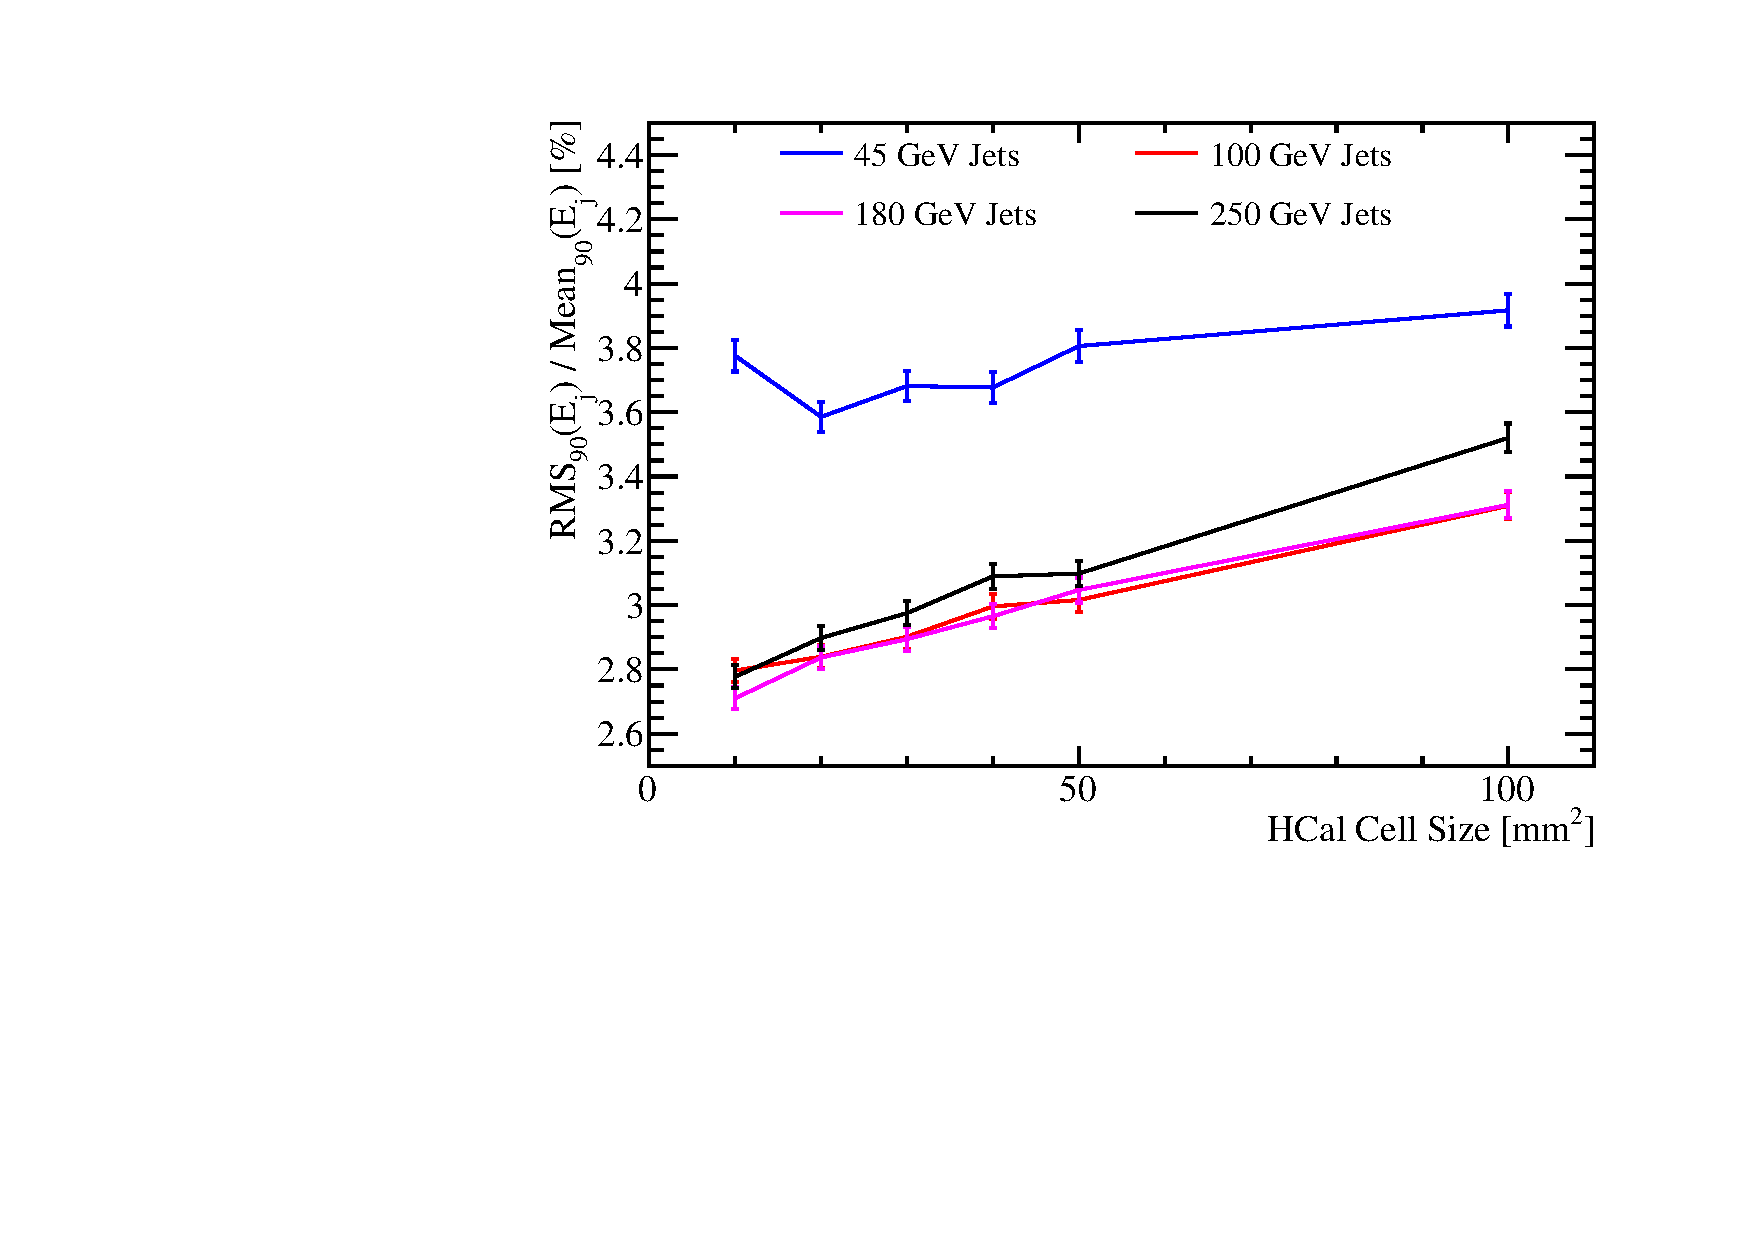
\includegraphics[width=0.5\textwidth]{OptimisationStudies/Plots/JetEnergyResolutions/JER_vs_HCalCellSize.pdf}}
\subfloat[]{\label{fig:jerhcalcelloptbadtrunc}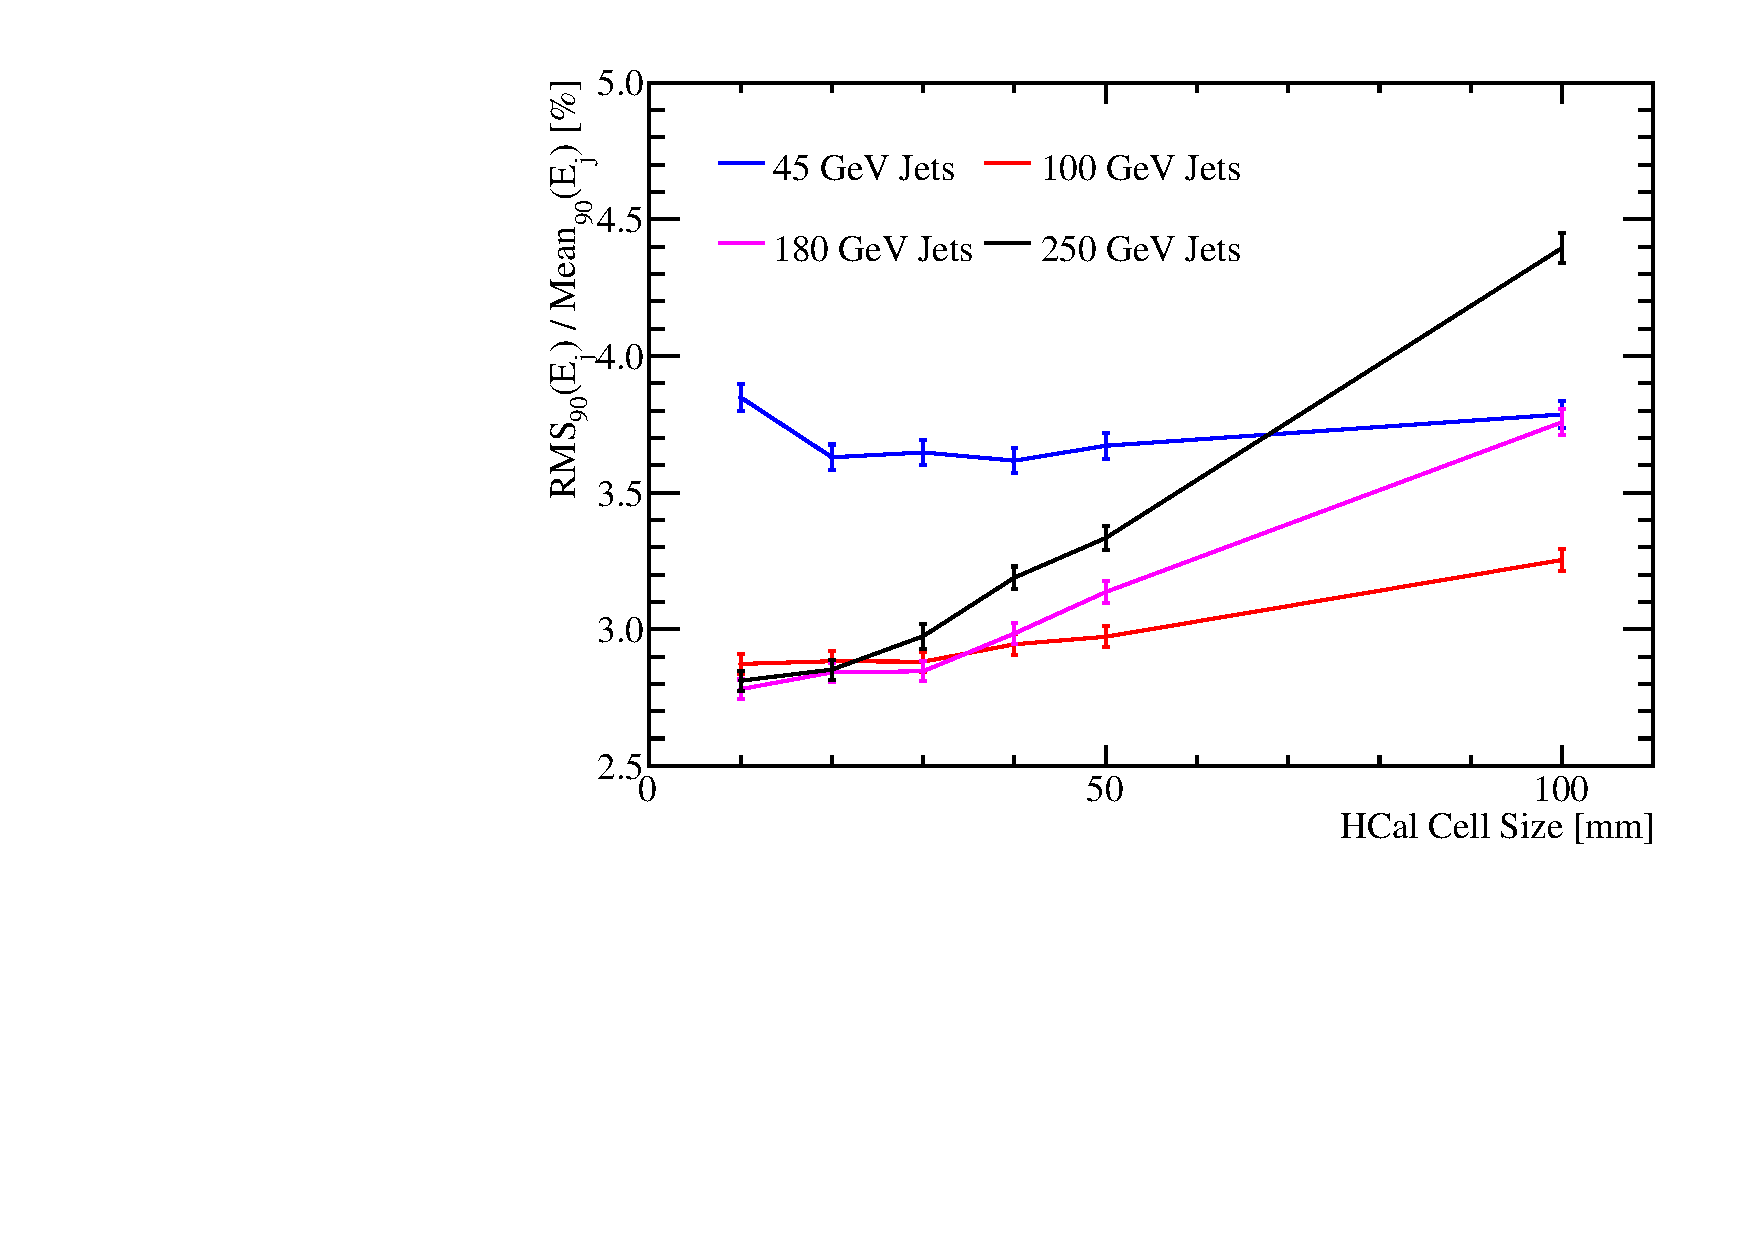
\includegraphics[width=0.5\textwidth]{EnergyEstimators/Plots/CellTruncation/JER_vs_HCalCellSizeBadTruncation.pdf}}
\caption[The jet energy resolution as a function of HCal cell size in the ILD detector model using a HCal hit energy truncation that is \protect\subref{fig:jerhcalcelloptgoodtrunc} optimised and \protect\subref{fig:jerhcalcelloptbadtrunc} fixed at 1~GeV.]{The jet energy resolution as a function of HCal cell size in the ILD detector model using a HCal hit energy truncation that is \protect\subref{fig:jerhcalcelloptgoodtrunc} optimised and \protect\subref{fig:jerhcalcelloptbadtrunc} fixed at 1~GeV.}
\label{fig:jerhcalcellopt}
\end{figure}

%========================================================================================

\subsection{Software Compensation}
\label{sec:softcomp}
Particle showers that are produced when a hadron interacts with a calorimeter contain two components \cite{Wigmans:2000vf}; an electromagnetic shower core, which originates from the production and decay of $\pi^{0}$s and $\eta$s, and a hadronic shower component originating from other interacting and decaying particles.  By identifying each of these components in the reconstruction, it is possible to modify their energies to give a compensating calorimeter response.  This technique known as software compensation.  

Software compensation achieves a compensating calorimeter response by applying weights, as introduced in equation \ref{equ:compensation}, that modify the energy of calorimeter hits in the HCal.  These weights increase the energy found in the hadronic hits to compensate for the undetectable energy component found in hadronic showers.  Additionally, these weights reduce the energy of spuriously high energy hits to minimise the impact of Landau fluctuations.  The weights vary as a function of the calorimeter hit energy density, $\rho^{i}$, and the uncompensated energy of the particle shower, $E_{Raw}$, where 
%
\begin{equation}
E_{Raw} & = \sum_{ECal \text{ } hits \text{, }i} E^{i}_{ECal} +\sum_{HCal \text{ } hits \text{, }i} E^{i}_{HCal} \text{ .}
\label{equ:eraw}
\end{equation}
%
\noindent  The electromagnetic and hadronic components of a hadronic particle shower are treated differently in this approach by applying wights that are sensitive to the energy density of the calorimeter hits.  Hits with large energy densities are likely to be part of the electromagnetic core, while low energy density hits are likely to be part of satellite hadronic hits around the electromagnetic shower core \cite{Adloff:2012gv}.  By tailoring the weights as a function of the energy density, a compensating calorimeter response can be obtained.  Figure \ref{fig:softcompeventdisplay} shows the electromagnetic and hadronic shower components, determined by the energy density of the calorimeter hits, for a hadronic shower in a 500~GeV Z$\rightarrow$uds di-jet event.  

\begin{figure}[h!]
\subfloat[]{\label{fig:softcompfulleventdisplay}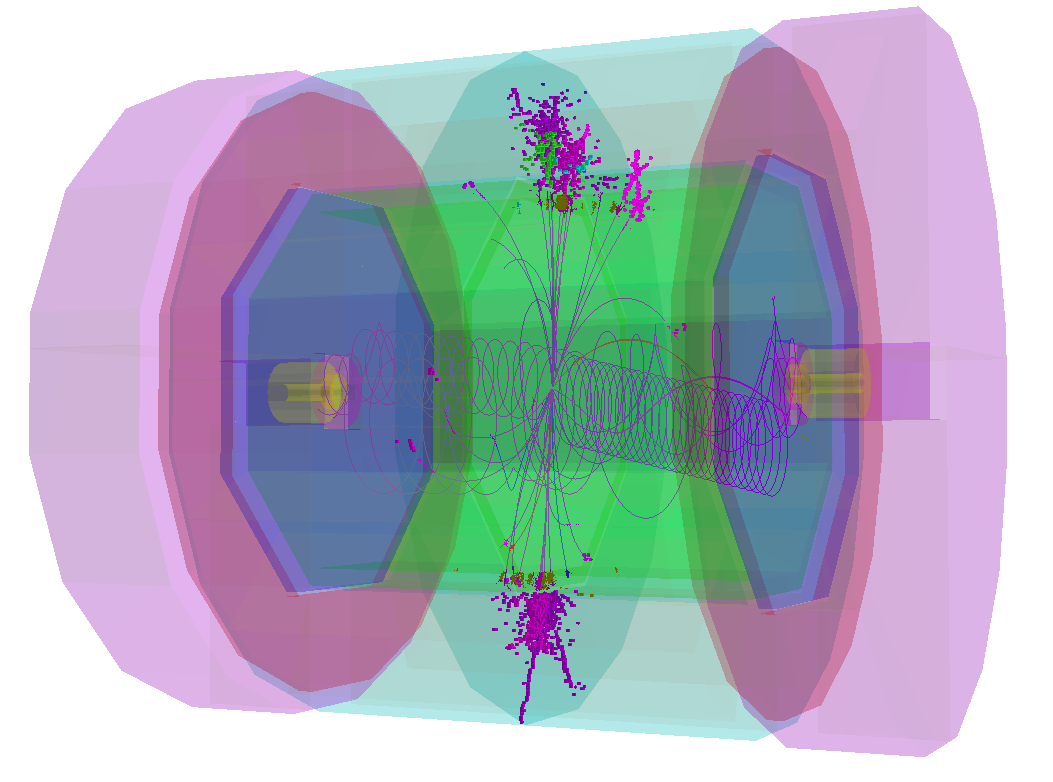
\includegraphics[width=0.5\textwidth]{EnergyEstimators/Plots/SoftComp/VisualDisplay/SoftComp1.png}}
\subfloat[]{\label{fig:softcompclustereventdisplay}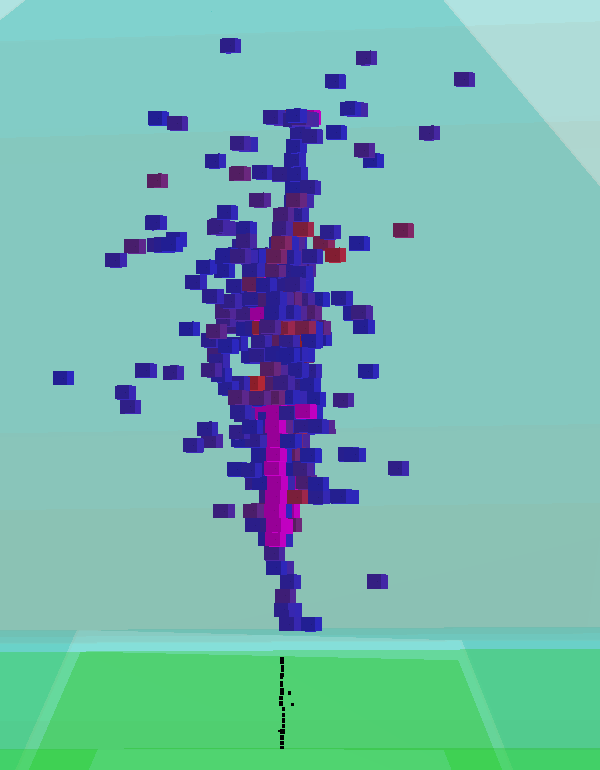
\includegraphics[width=0.3\textwidth]{EnergyEstimators/Plots/SoftComp/VisualDisplay/SoftComp3.png}}
\caption[An event display for a 500~GeV Z$\rightarrow$uds di-jet event reconstructed using the nominal ILD detector.  \protect\subref{fig:softcompfulleventdisplay} The full event environment.  \protect\subref{fig:softcompclustereventdisplay} A single hadronic cluster from the same event where shading indicates the energy density in the HCal.  High energy density cells are coloured red, while lower energy density cells are coloured blue.  All ECal hits are shaded black.  The high energy density electromagnetic core of the selected hadronic cluster is clearly visible.]{An event display for a 500~GeV Z$\rightarrow$uds di-jet event reconstructed using the nominal ILD detector.  \protect\subref{fig:softcompfulleventdisplay} The full event environment.  \protect\subref{fig:softcompclustereventdisplay} A single hadronic cluster from the same event where shading indicates the energy density in the HCal.  High energy density cells are coloured red, while lower energy density cells are coloured blue.  All ECal hits are shaded black.  The high energy density electromagnetic core of the selected hadronic cluster is clearly visible.}
\label{fig:softcompeventdisplay}
\end{figure}

The software compensation weights also depend on $E_{Raw}$, the total raw cluster energy, to account for the sensitivity of the hit energy density distribution on the total particle shower energy.  For hadronic showers, the fraction of the total energy carried in the electromagnetic core increases as the total shower energy increases \cite{Wigmans:2000vf}, therefore a dependancy of the weights on $E_{Raw}$ is needed to obtain a compensating calorimeter response across a wide range of energies.  

The precise form of the weights used in this technique are \cite{Adloff:2012gv}
%
\begin{equation}
\omega(E_{Raw}, \rho) = p_{1}(E_{Raw}) \times \text{exp}(p_{2}(E_{Raw}) \times \rho) + p_{3}(E_{Raw}) \text{ ,} \\
\label{equ:softcompweight}
\end{equation}
\noindent with
\begin{equation}
p_{1}(E_{Raw}) = p_{11} + p_{12} \times E_{Raw} + p_{13} \times E_{Raw}^{2} \\
p_{2}(E_{Raw}) = p_{21} + p_{22} \times E_{Raw} + p_{23} \times E_{Raw}^{2} \\
p_{3}(E_{Raw}) = \frac{p_{31}}{p_{32} + \text{exp}(p_{33} \times E_{Raw})}\text{ ,}
\end{equation}
\noindent where $p_{\alpha\beta}$ are constants and
\begin{equation}
E_{Raw} & = \sum_{ECal \text{ } hits \text{, }i} E^{i}_{ECal} +\sum_{HCal \text{ } hits \text{, }i} E^{i}_{HCal} \text{ .}
\end{equation}
%
\noindent The parameters $p_{\alpha\beta}$ were determined by minimising $\chi^{2}(p_{\alpha\beta})$ where
%
\begin{equation}
\chi^{2}(p_{\alpha\beta}) = \sum_{Events} \bigg( \frac{(E^{SC}_{Cluster}(p_{\alpha\beta}) - E_{MC})}{0.5 \times \sqrt{E_{MC}}} \bigg)^{2}
\end{equation}
%
where the sum runs over single $K^{0}_{L}$ events that ranged in energy from 10 to 100~GeV in steps of 10~GeV.  At each energy the same number of events was used to avoid biasing to particular energies.  In each event, $E^{SC}_{Cluster}$ is the software compensated energy estimator for the reconstructed event and $E_{MC}$ is the MC energy of the $K^{0}_{L}$.  Normalising the deviation of $E^{SC}_{Cluster}$ from $E_{MC}$ by the stochastic term in the HCal energy resolution, $\sim 50\% \times \sqrt{E}$, made sure events of different MC energy contributed the same weight to $\chi^{2}$.  

Figure \ref{fig:softcompweights} shows $\omega$ as a function of $\rho$ for selected values of $E_{Raw}$ and figure \ref{fig:softcompparams} shows $p_{1}$, $p_{2}$ and $p_{3}$ as a function of $E_{Raw}$.  These weights shown in figures \ref{fig:softcompweights} and \ref{fig:softcompparams} were obtained by training the software compensation technique on samples simulated using the nominal ILD detector model.  Figure \ref{fig:softcompweights} shows that the high energy density hits are being reduced in energy to compensate for the effects of Landau fluctuations, while the low energy density hits are being increased in weight to compensate for the undetectable energy component found in hadronic showers.  Furthermore, the weights vary as a function of the raw hadronic shower energy to account for the changing energy density topology of hadronic showers with increasing shower energy.

\begin{figure}[h!]
\subfloat[]{\label{fig:softcompparam1}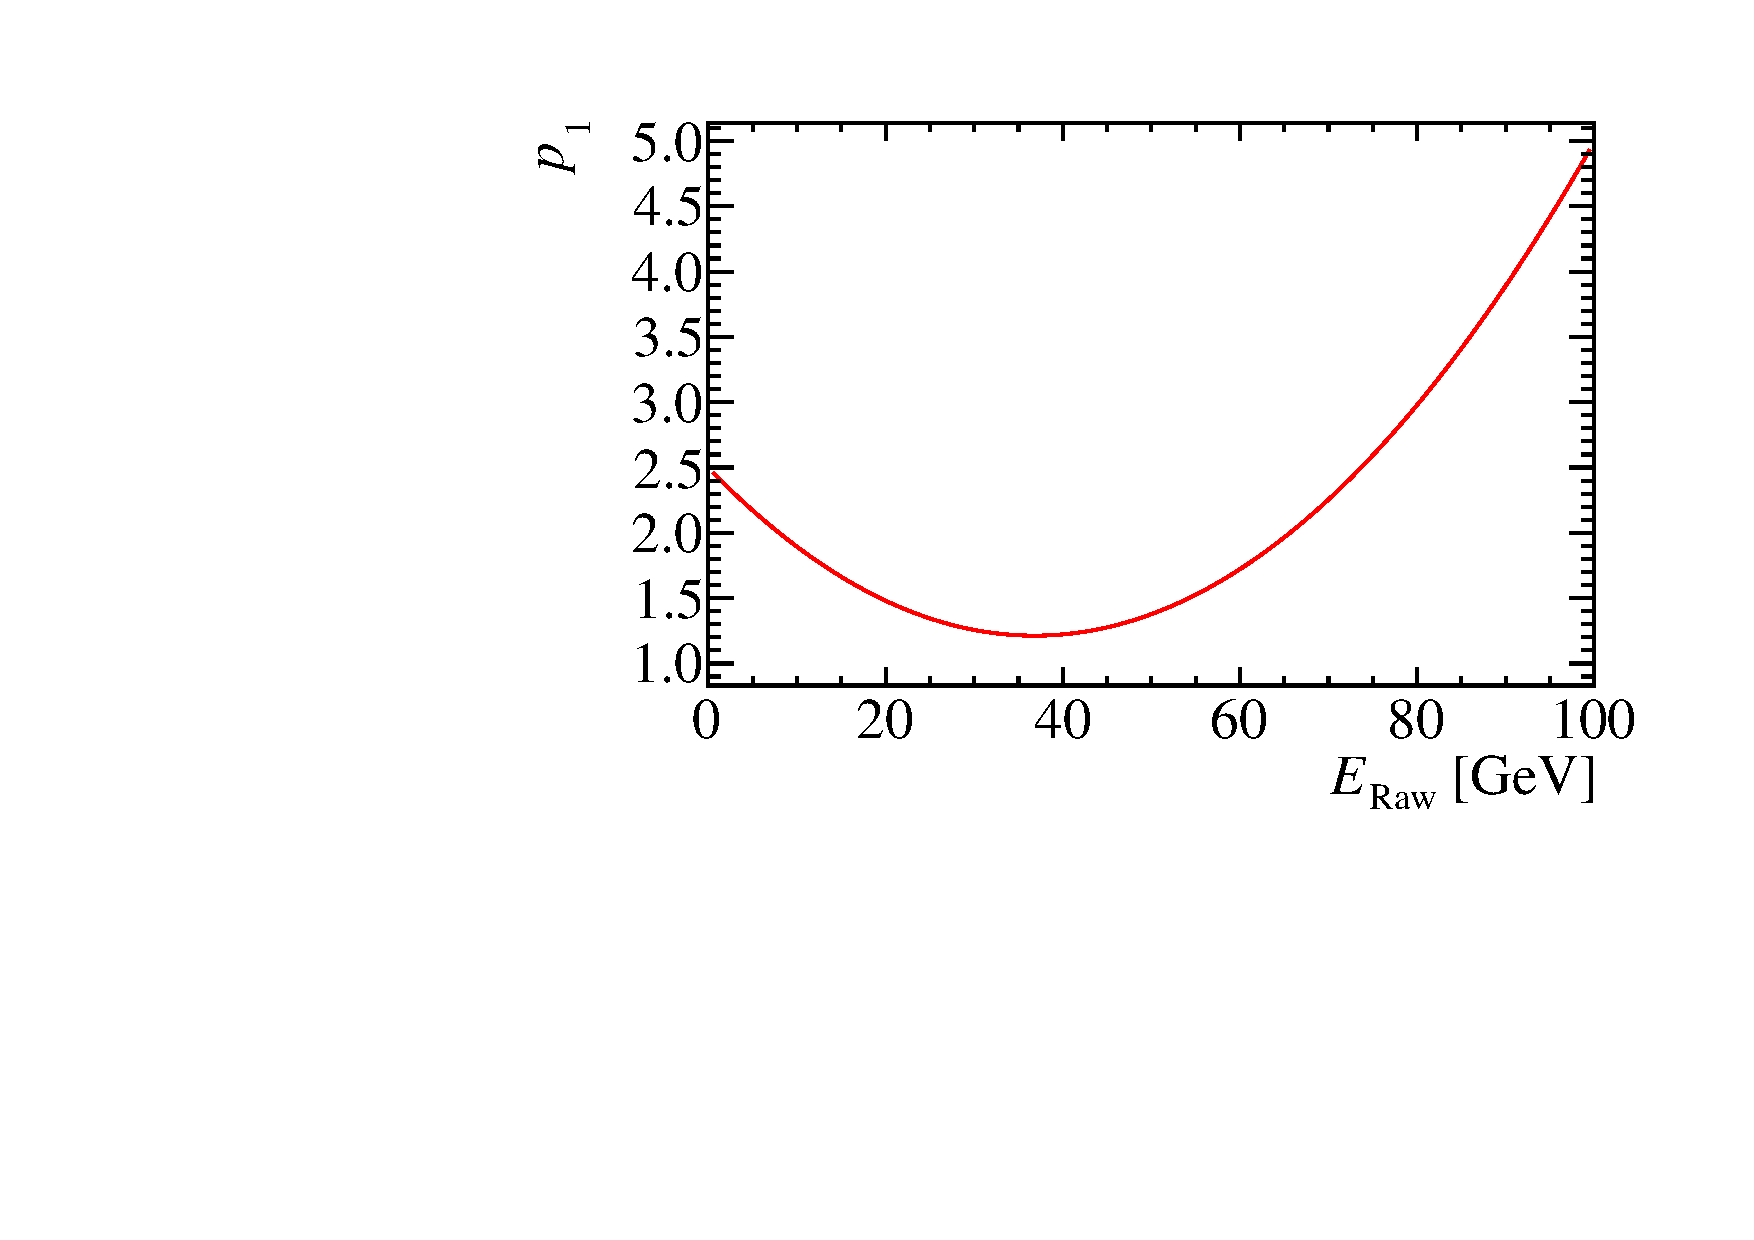
\includegraphics[width=0.33\textwidth]{EnergyEstimators/Plots/SoftComp/Weights/SoftwareCompensationParam1.pdf}}
\subfloat[]{\label{fig:softcompparam2}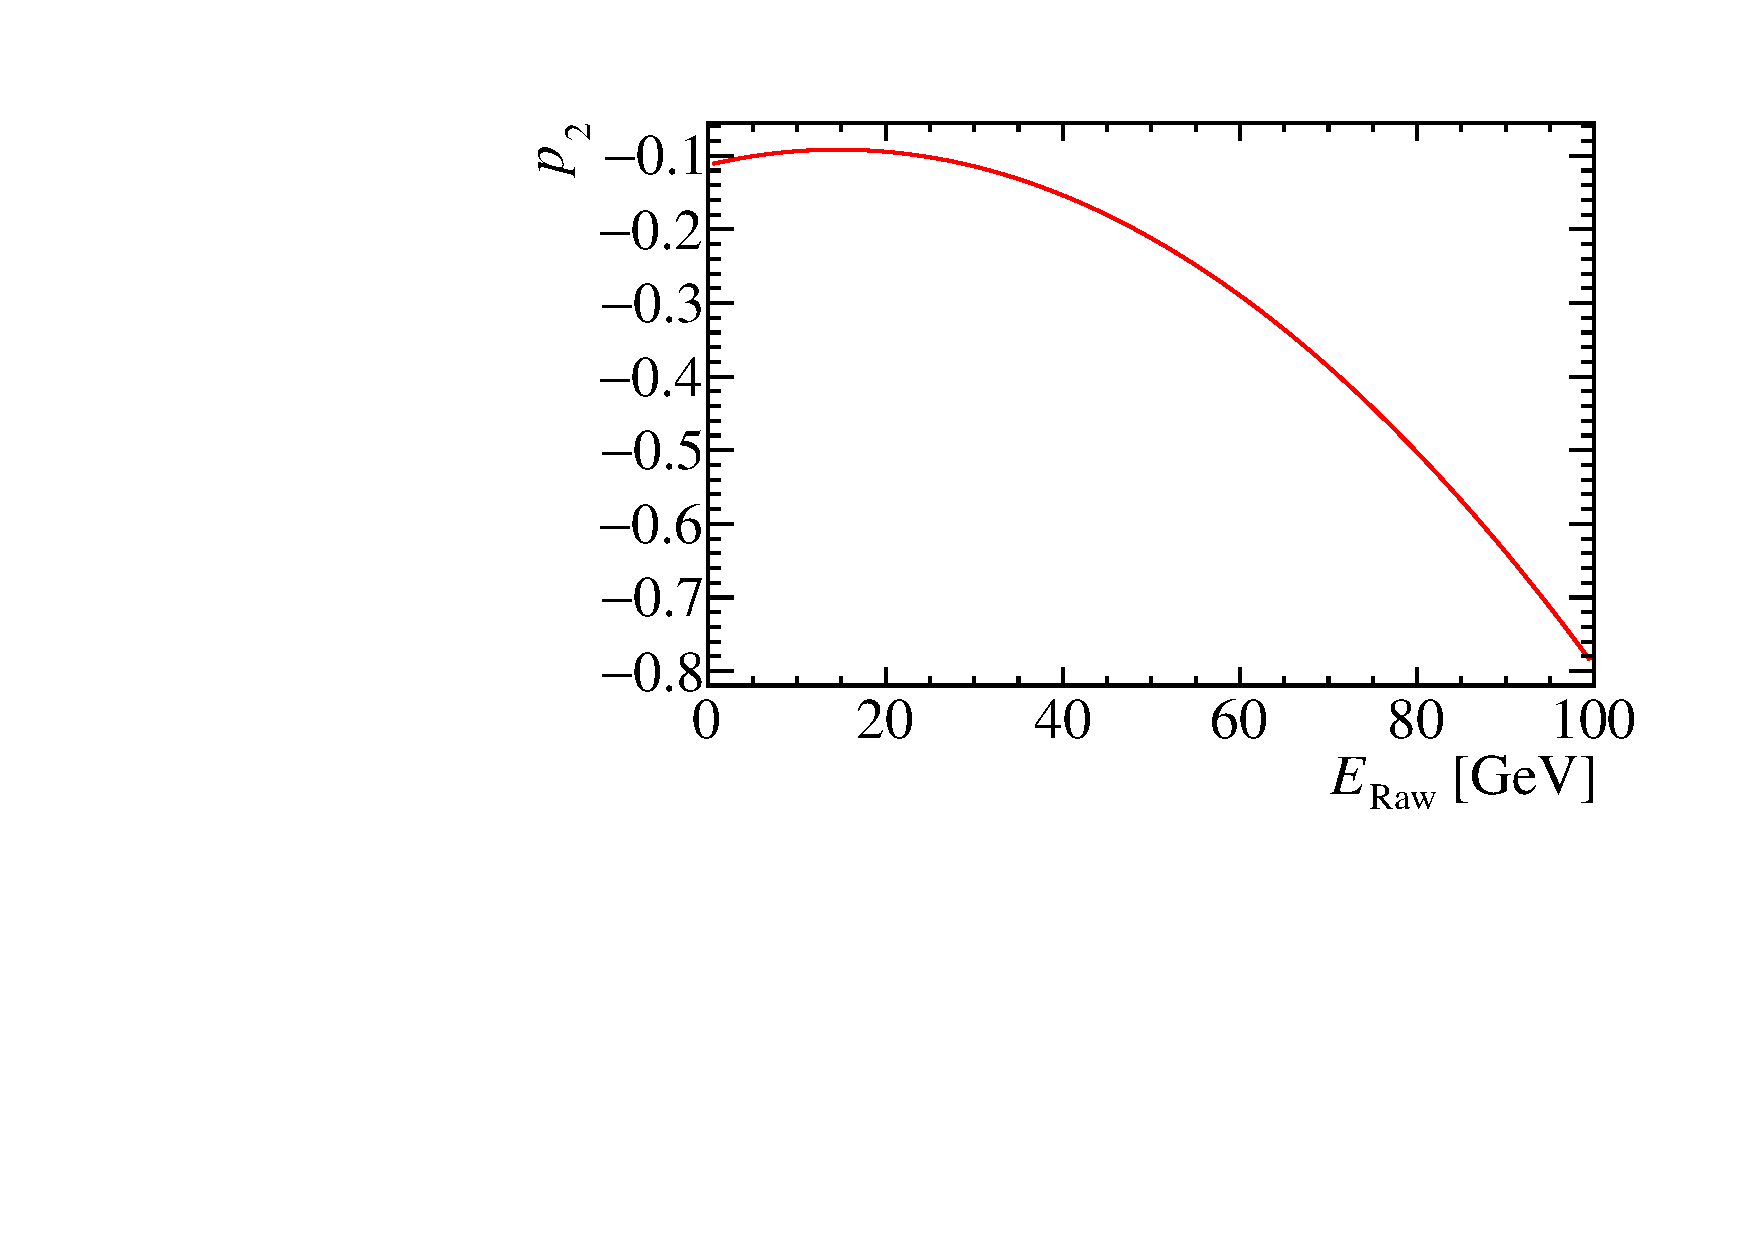
\includegraphics[width=0.33\textwidth]{EnergyEstimators/Plots/SoftComp/Weights/SoftwareCompensationParam2.pdf}}
\subfloat[]{\label{fig:softcompparam3}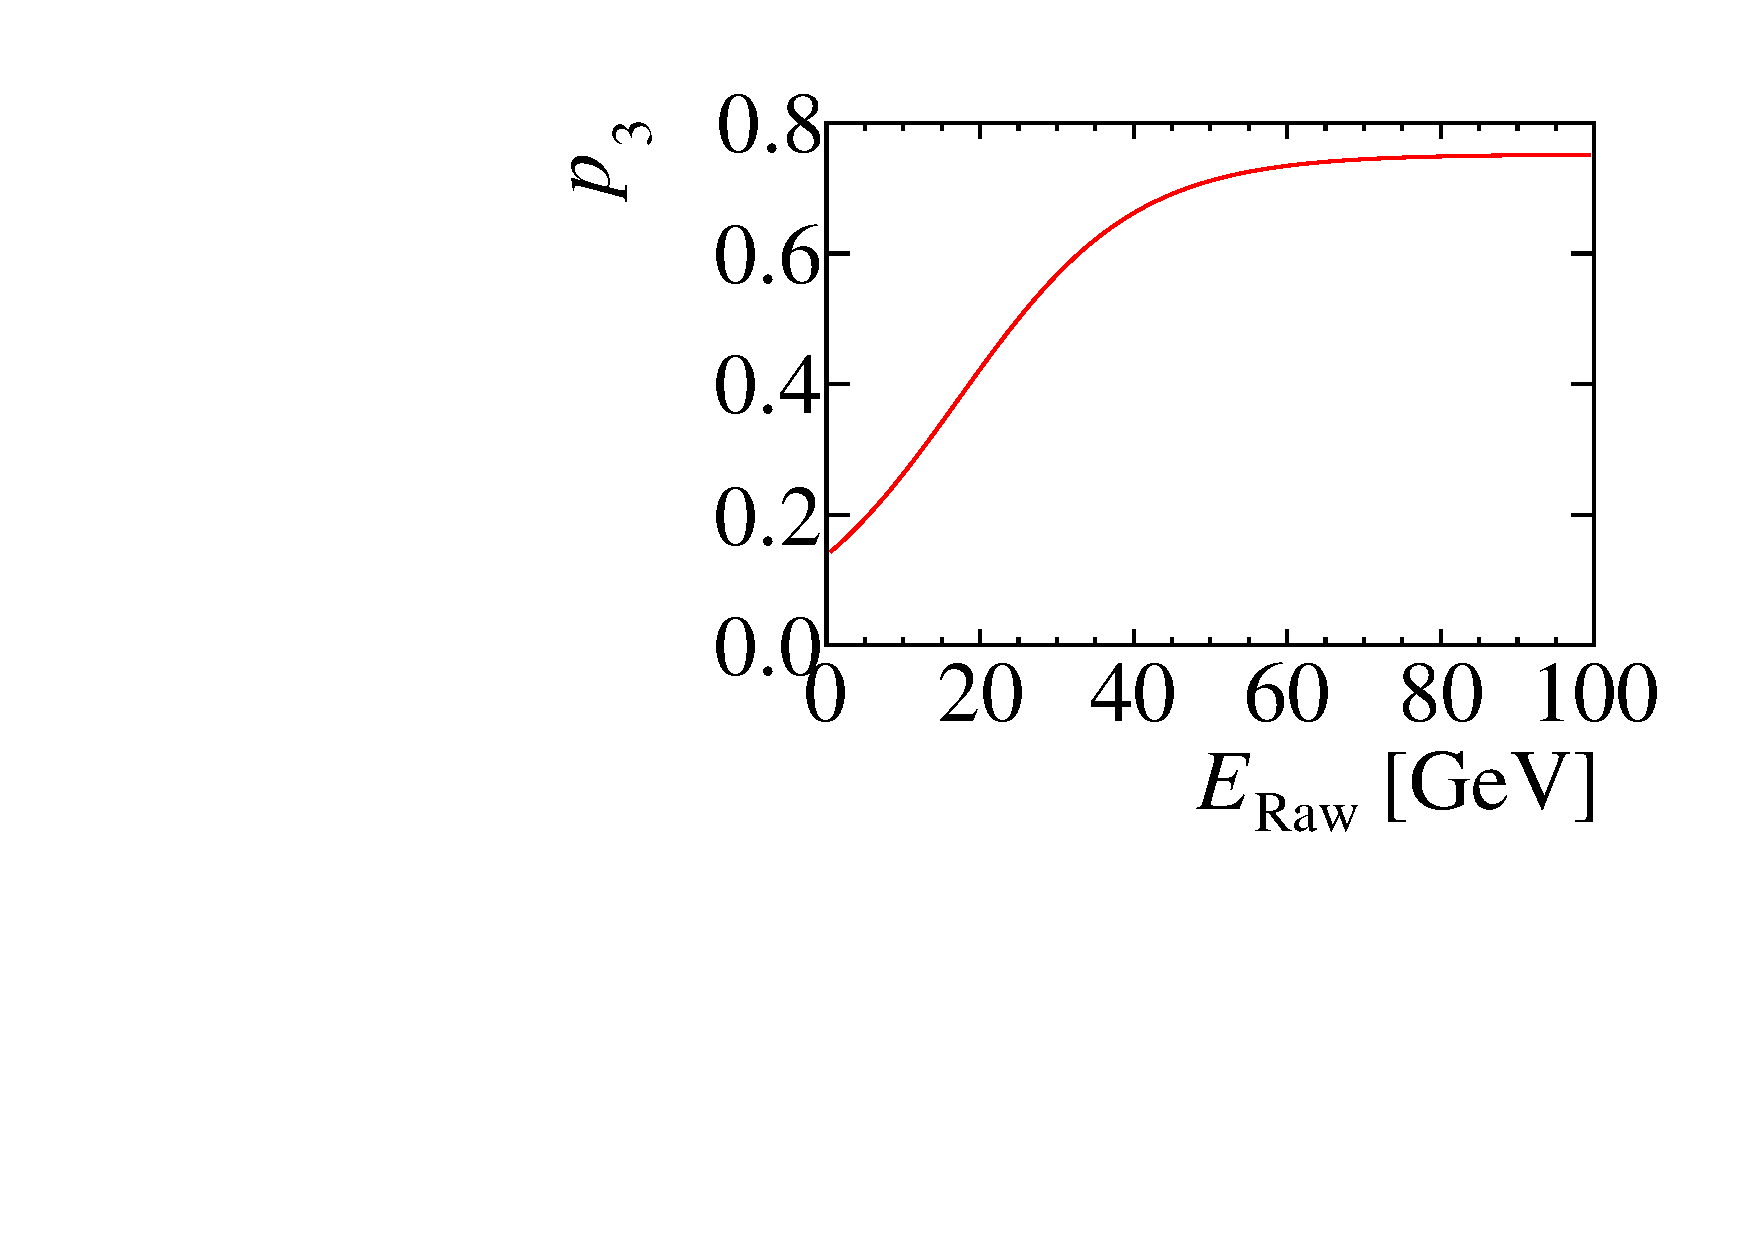
\includegraphics[width=0.33\textwidth]{EnergyEstimators/Plots/SoftComp/Weights/SoftwareCompensationParam3.pdf}}
\caption[The software compensation parameters \protect\subref{fig:softcompparam1} $p_{1}$, \protect\subref{fig:softcompparam2} $p_{2}$ and \protect\subref{fig:softcompparam3} $p_{3}$ as a function of $E_{Raw}$, the total raw cluster energy.  These weights were obtained by training the software compensation technique on samples simulated using the nominal ILD detector model.]{The software compensation parameters \protect\subref{fig:softcompparam1} $p_{1}$, \protect\subref{fig:softcompparam2} $p_{2}$ and \protect\subref{fig:softcompparam3} $p_{3}$ as a function of $E_{Raw}$, the total raw cluster energy.  These weights were obtained by training the software compensation technique on samples simulated using the nominal ILD detector model.}
\label{fig:softcompparams}
\end{figure}

\begin{figure}[h!]
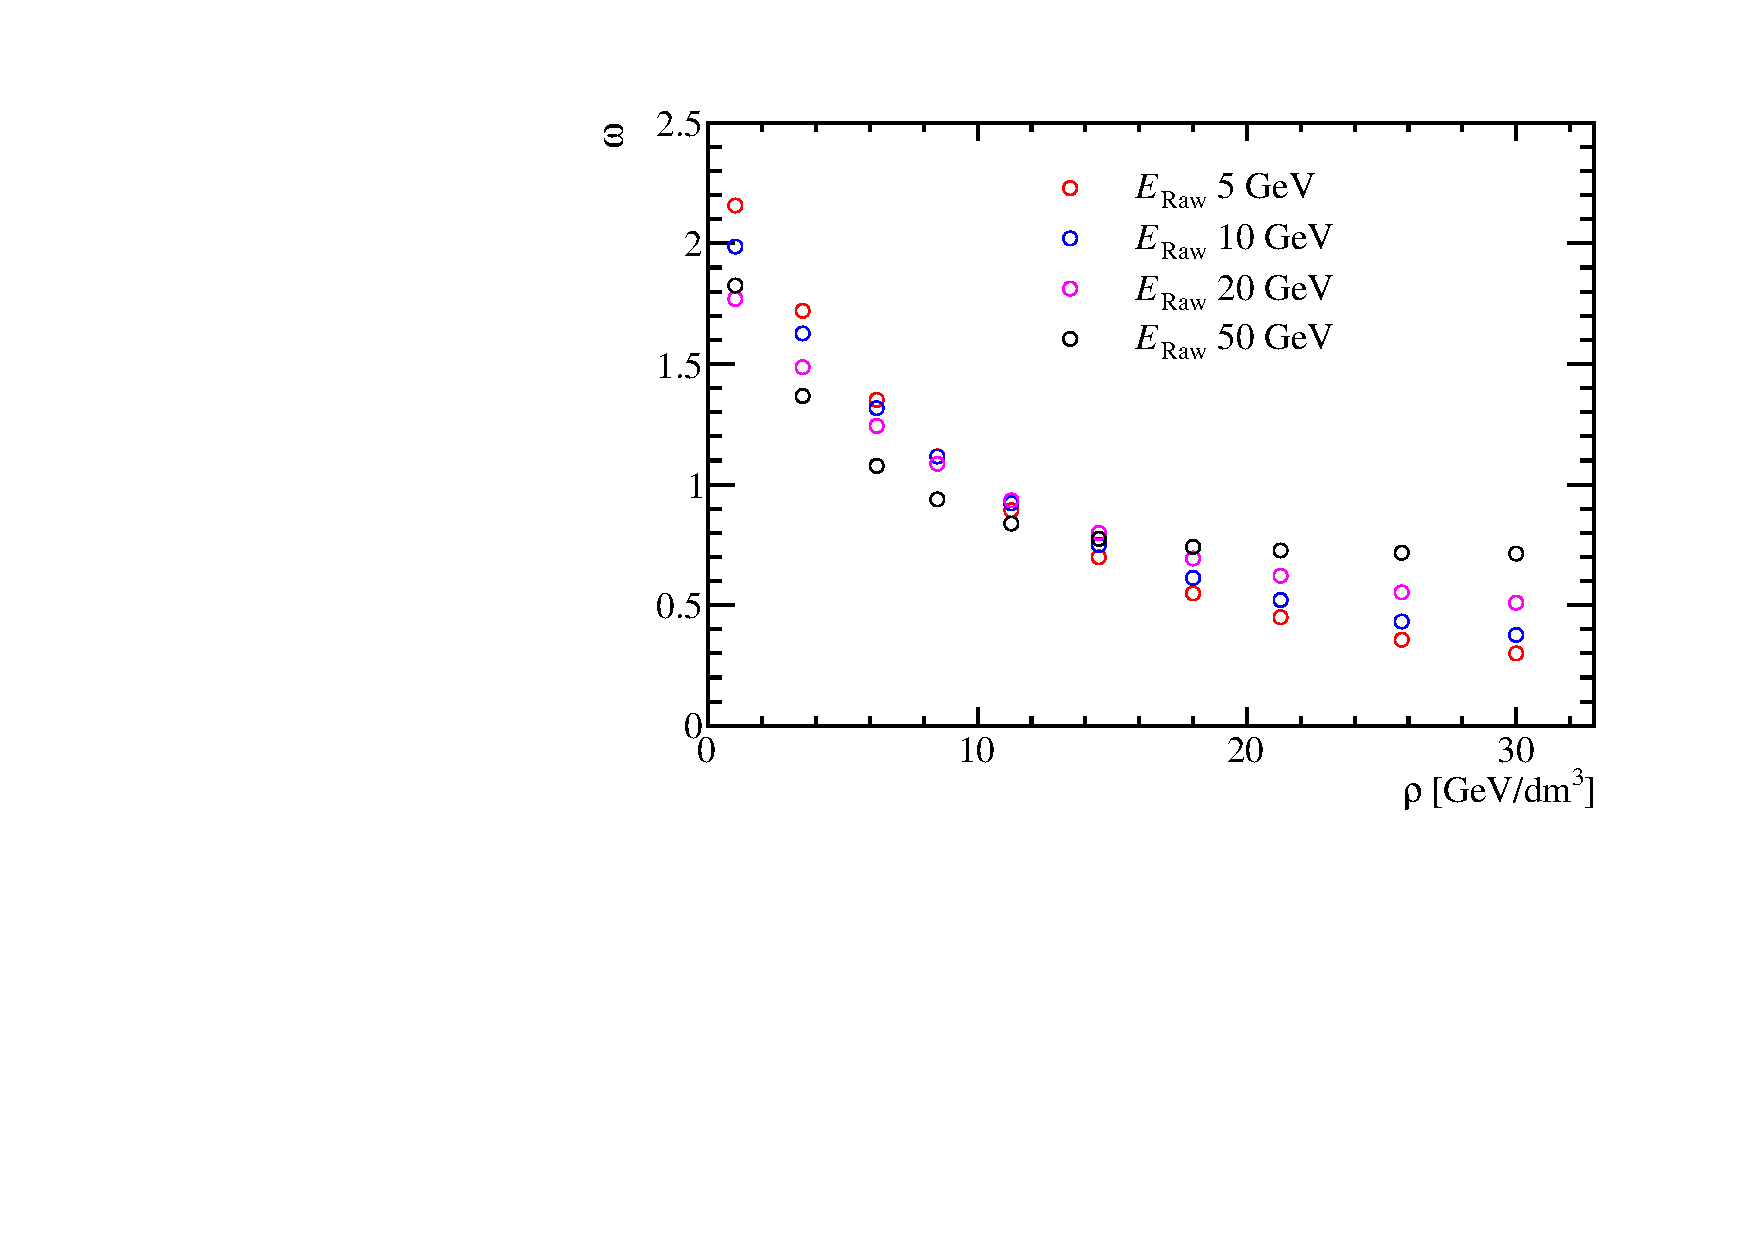
\includegraphics[width=0.75\textwidth]{EnergyEstimators/Plots/SoftComp/Weights/SoftwareCompensationWeights.pdf}
\caption[The software compensation weight applied to a calorimeter hit as a function of calorimeter hit energy density for various cluster energies.]{The software compensation weight applied to a calorimeter hit as a function of calorimeter hit energy density for various cluster energies.}
\label{fig:softcompweights}
\end{figure}

The software compensation technique is applied in the PandoraPFA framework in the form of an energy correction function, which means whenever the energy of a cluster of hits is considered by PandoraPFA the software compensated energy is used.  Applying software compensation in this way benefits the detector energy resolution in two ways; firstly, the intrinsic energy resolution of the detector improves and secondly, the confusion contribution to the energy resolution is reduced.

As software compensation only modifies the energy of HCal hits there is freedom to apply further energy corrections to the ECal hits.  Applying the "Clean Clusters" logic, described in section \ref{sec:legacycorrections}, to the ECal hits alongside software compensation was found to be beneficial to the jet energy resolution.  Therefore, the application of software compensation within PandoraPFA implicitly involves the application of the "Clean Clusters" logic to the ECal hits.  

Software compensation was tuned using a maximum $K^{0}_{L}$ energy of 100~GeV, therefore, it is only applied to clusters where $E_{Raw} < 100$~GeV; sensible behaviour outside this range cannot be ensured.  While it would be possible to modify the energy range of the training sample to go to higher energies, hadronic clusters with energy greater than 100~GeV will be rare at the ILC-like energies, i.e. $\sqrt{s} \leq 500$~GeV, considered here.

%========================================================================================

\subsubsection{Impact on Single Particle Energy Resolution}
\label{sec:softcomper}
Figure \ref{fig:ersoftcomp} shows the energy resolution as a function of MC energy for single $K^{0}_{L}$ events obtained using the various energy correction configurations in PandoraPFA.  When comparing the energy resolution given by software compensation to that obtained using no energy corrections, it can be seen that software compensation offers an improvement in the energy resolution of $\sim 15 \%$ across the energy range considered.  The uniformity of this improvement is encouraging, indicating that software compensation is achieving a compensating calorimeter response across this wide range of energies.  

Comparing the performance of software compensation to the legacy corrections, described in section \ref{sec:legacycorrections}, it can be seen that software compensation gives a better energy resolution across almost the entire range of energies considered.  The only exception to this is around $E_{K^{0}_{L}} \sim 50$~GeV where the performance of software compensation and the legacy corrections are comparable.  By removing the hit truncation from the legacy options it is clear that the changes in energy resolution when using the legacy options are being driven by the hit truncation.  This makes the trend in energy resolution observed using the legacy corrections clear as, at low $K^{0}_{L}$ energies, very few hits are affected by the truncation so the performance is comparable to not using any energy corrections.  At high $K^{0}_{L}$ energies, the truncation is too aggressive and removes energy from hits that are not spuriously high leading to a worsening energy resolution.  Between these two extremes, $E_{K^{0}_{L}} \sim 50$~GeV, the truncation works ideally and the improvement in energy resolution when using the legacy corrections is the largest.  

\begin{figure}[h!]
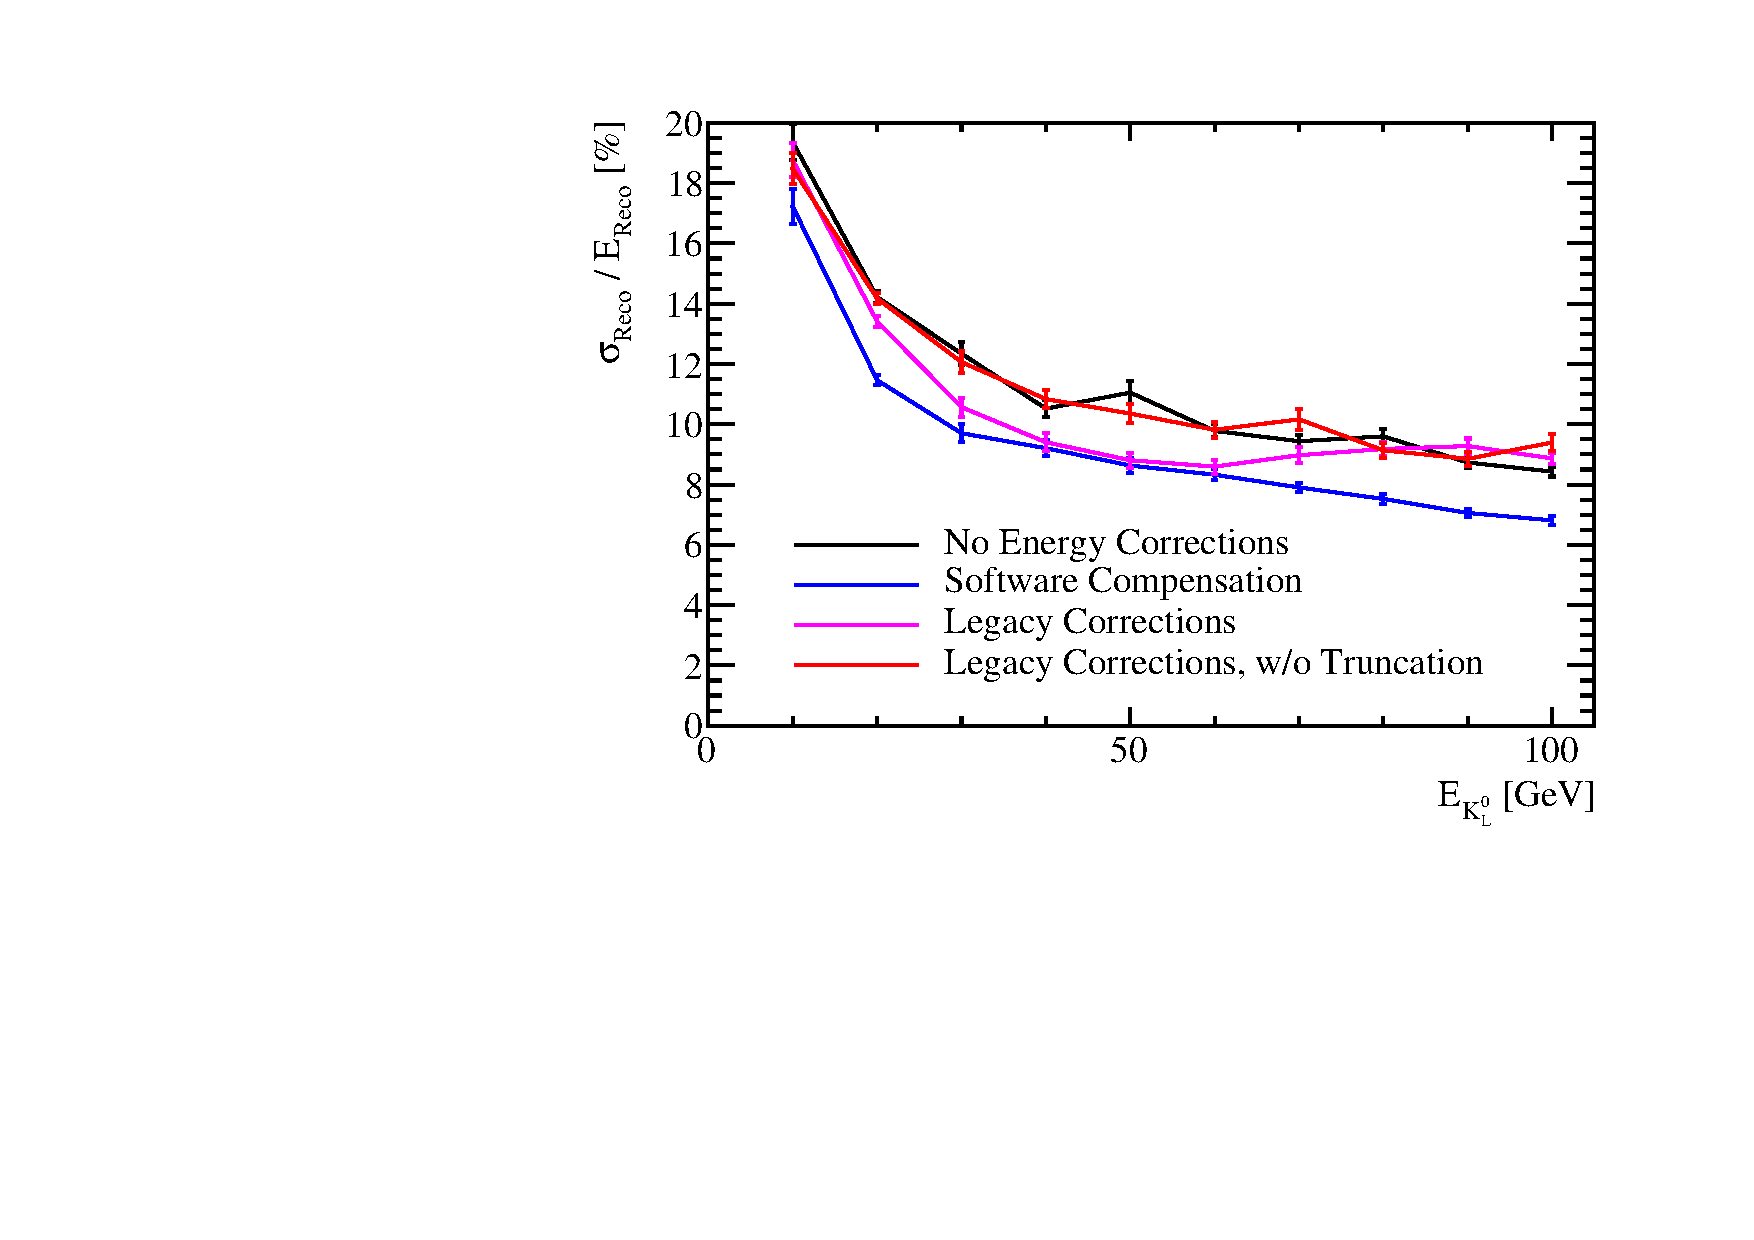
\includegraphics[width=0.75\textwidth]{EnergyEstimators/Plots/SoftComp/EnergyResolution/ER_vs_Kaon0LSoftComp_Kaon0L.pdf}
\caption[The energy resolution as a function of the MC energy for single $K^{0}_{L}$ events using various energy correction settings.  The black line represents no energy corrections, the blue line represents software compensation, the magenta line represents the legacy energy corrections and the red line represents the legacy corrections without the HCal hit energy truncation.  The nominal ILD detector model was used in these simulations.]{The energy resolution as a function of the MC energy for single $K^{0}_{L}$ events using various energy correction settings.  The black line represents no energy corrections, the blue line represents software compensation, the magenta line represents the legacy energy corrections and the red line represents the legacy corrections without the HCal hit energy truncation.  The nominal ILD detector model was used in these simulations.}
\label{fig:ersoftcomp}
\end{figure}

%========================================================================================

\subsubsection{Impact on Jet Energy Resolution}
The improvements in the intrinsic energy resolution of the detector observed when using software compensation will propagate into the reconstruction of jets.  Figure \ref{fig:jersoftcomp} shows the jet energy resolution as a function of jet energy when using selected energy correction configurations in PandoraPFA.  It can be seen that software compensation improves the jet energy resolution by $\sim 15 \%$ across the energy range considered in comparison to using no energy corrections.  Furthermore, software compensation offers an improvement in the jet energy resolution of the order of 5\% for jet energies $\gtrapprox 100$~GeV in comparison to the legacy corrections, which prior to the development of software compensation had given the best jet energy resolutions.

\begin{figure}[h!]
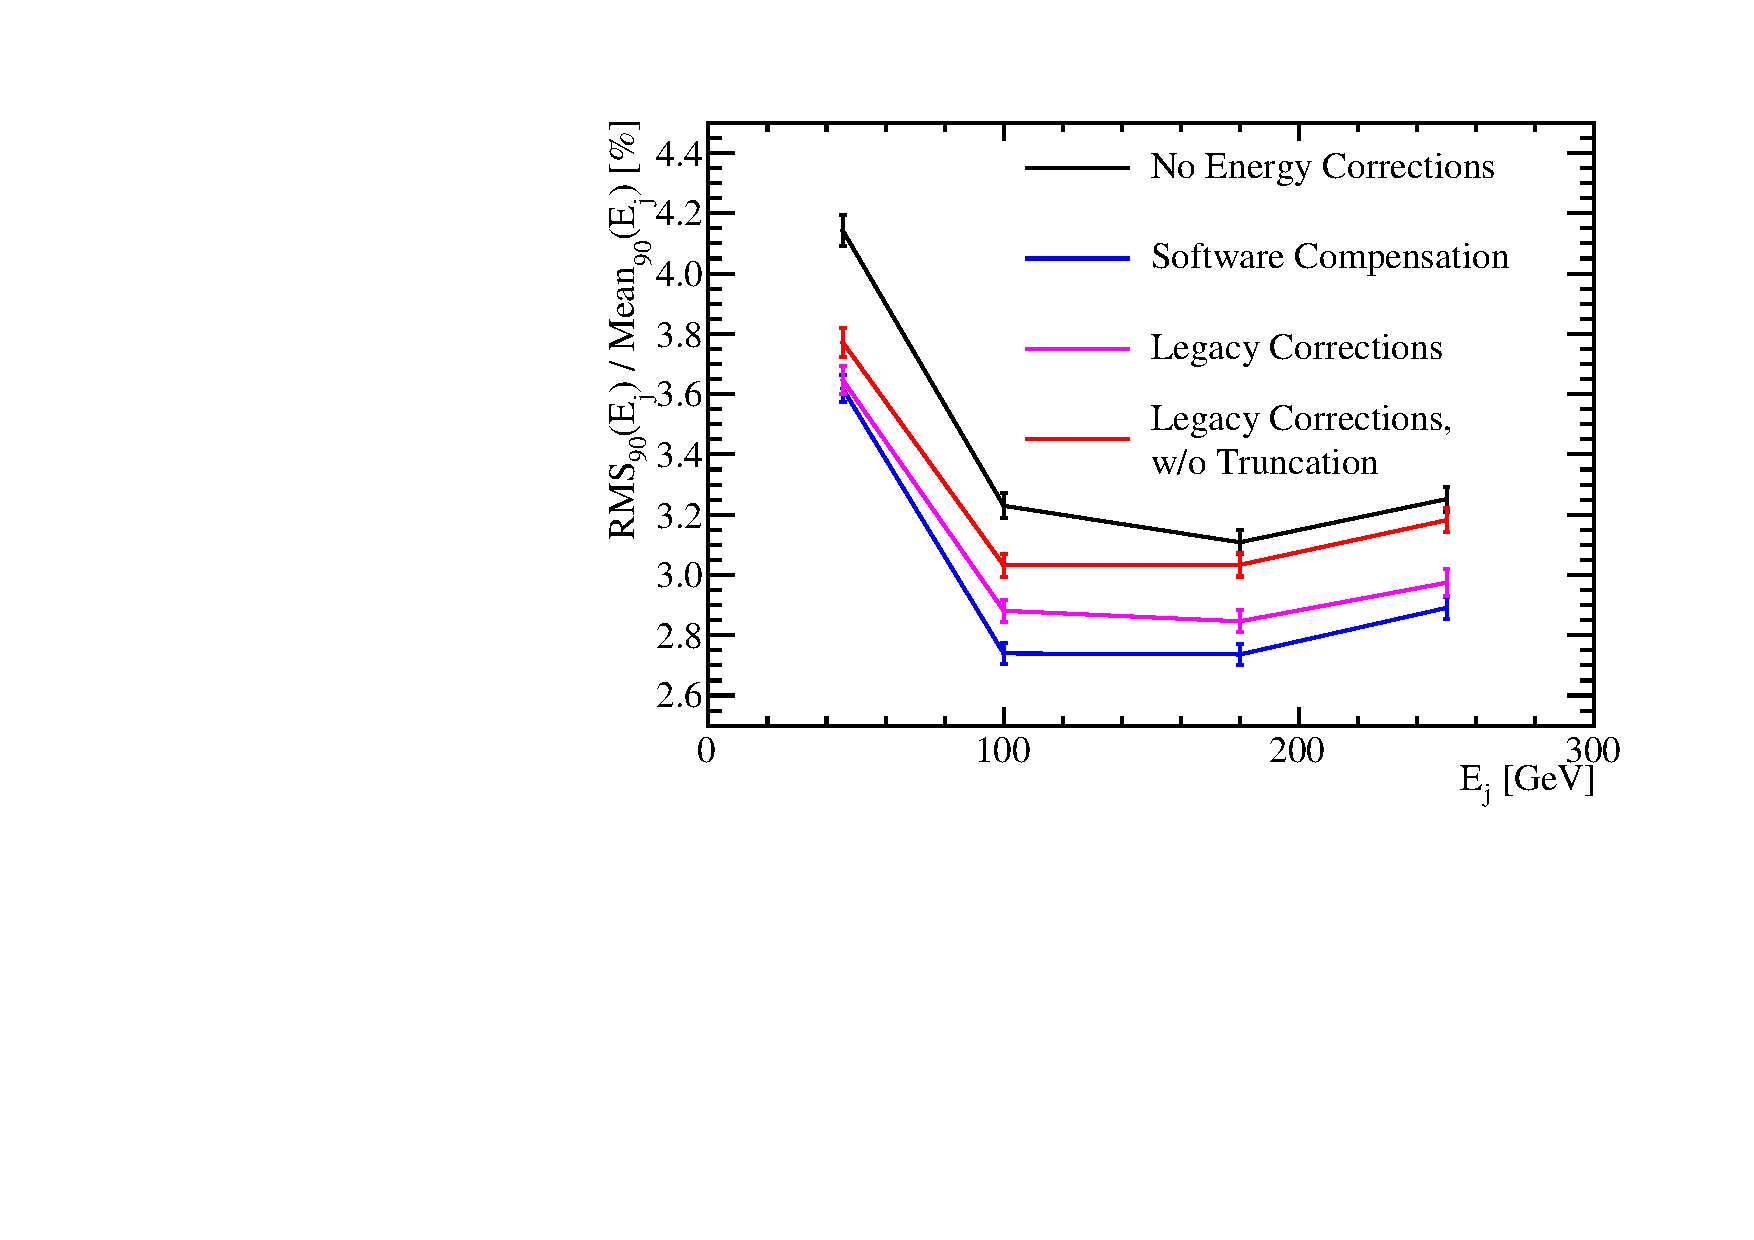
\includegraphics[width=0.75\textwidth]{EnergyEstimators/Plots/SoftComp/JetEnergyResolution/JER_vs_JetEnergy_Default.pdf}
\caption[The jet energy resolution as a function of the jet energy for a variety of different energy correction options.  The black line represents no energy corrections, the blue line represents software compensation, the magenta line represents the legacy energy corrections and the red line represents the legacy corrections without the HCal hit energy truncation.  The nominal ILD detector model was used in these simulations.]{The jet energy resolution as a function of the jet energy for a variety of different energy correction options.  The black line represents no energy corrections, the blue line represents software compensation, the magenta line represents the legacy energy corrections and the red line represents the legacy corrections without the HCal hit energy truncation.  The nominal ILD detector model was used in these simulations.}
\label{fig:jersoftcomp}
\end{figure}

Figure \ref{fig:jerbreakdownsoftcomp} shows the intrinsic energy resolution and confusion contributions to the jet energy resolution as a function of jet energy when using selected energy correction configurations in PandoraPFA.  The intrinsic energy resolution contribution shows that software compensation is significantly better than all other energy corrections options, which is to be expected from the energy resolution studies presented in section \ref{sec:softcomper}.  When compared to the legacy energy corrections, software compensation improves the intrinsic energy resolution by up to 12\% across the energy range considered, with the largest improvement occurring for 100~GeV jets.  As jets contain a broad spectrum of hadronic cluster energies, there is no jet energy for which the intrinsic energy resolution of the detector is comparable between the legacy corrections and software compensation.  The confusion contributions to the jet energy resolution when using software compensation and the legacy corrections are almost identical.  This indicates that the improvement seen in the jet energy resolution when comparing software compensation to the legacy corrections, shown in figure \ref{fig:jersoftcomp}, is being driven by the intrinsic energy resolution.  

The "Clean Clusters" and "Scale Hot Hadrons" energy corrections, i.e. the legacy corrections without the HCal hit energy truncation, benefits the pattern recognition by reducing the confusion contribution.  The confusion contribution is reduced by $\sim$18\% for 45.5~GeV jets using these energy corrections, however, as the jet energy increases the magnitude of this improvement decreases, such that at 250~GeV jets no improvement is seen.  These corrections do not significantly affect the intrinsic energy resolution of the detector.  As these corrections benefit pattern recognition, selected aspects of their logic is applied to ECal hits in the software compensation energy correction as previously discussed.

\begin{figure}[h!]
\subfloat[]{\label{fig:jerbreakdownsoftcomp1}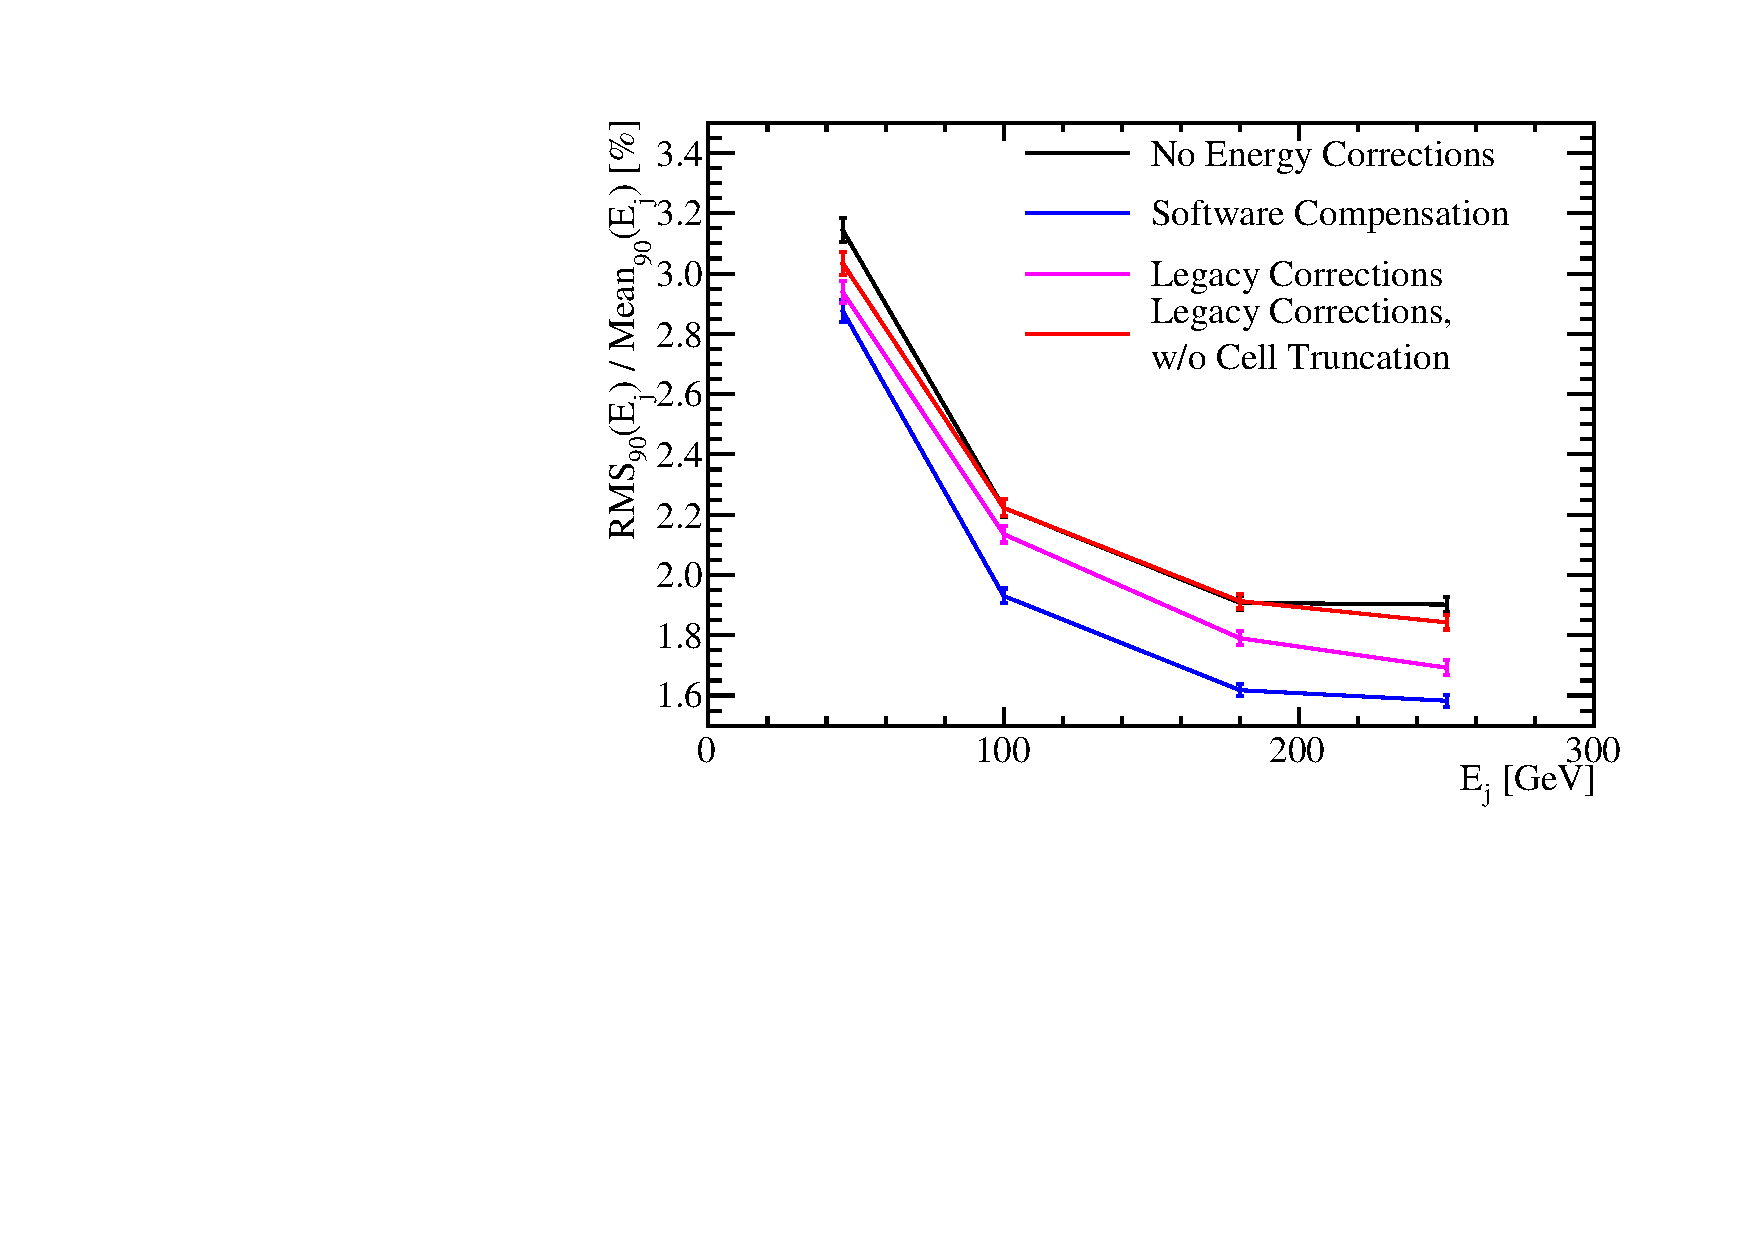
\includegraphics[width=0.5\textwidth]{EnergyEstimators/Plots/SoftComp/JetEnergyResolution/JER_vs_JetEnergy_PerfectPFA.pdf}}
\subfloat[]{\label{fig:jerbreakdownsoftcomp2}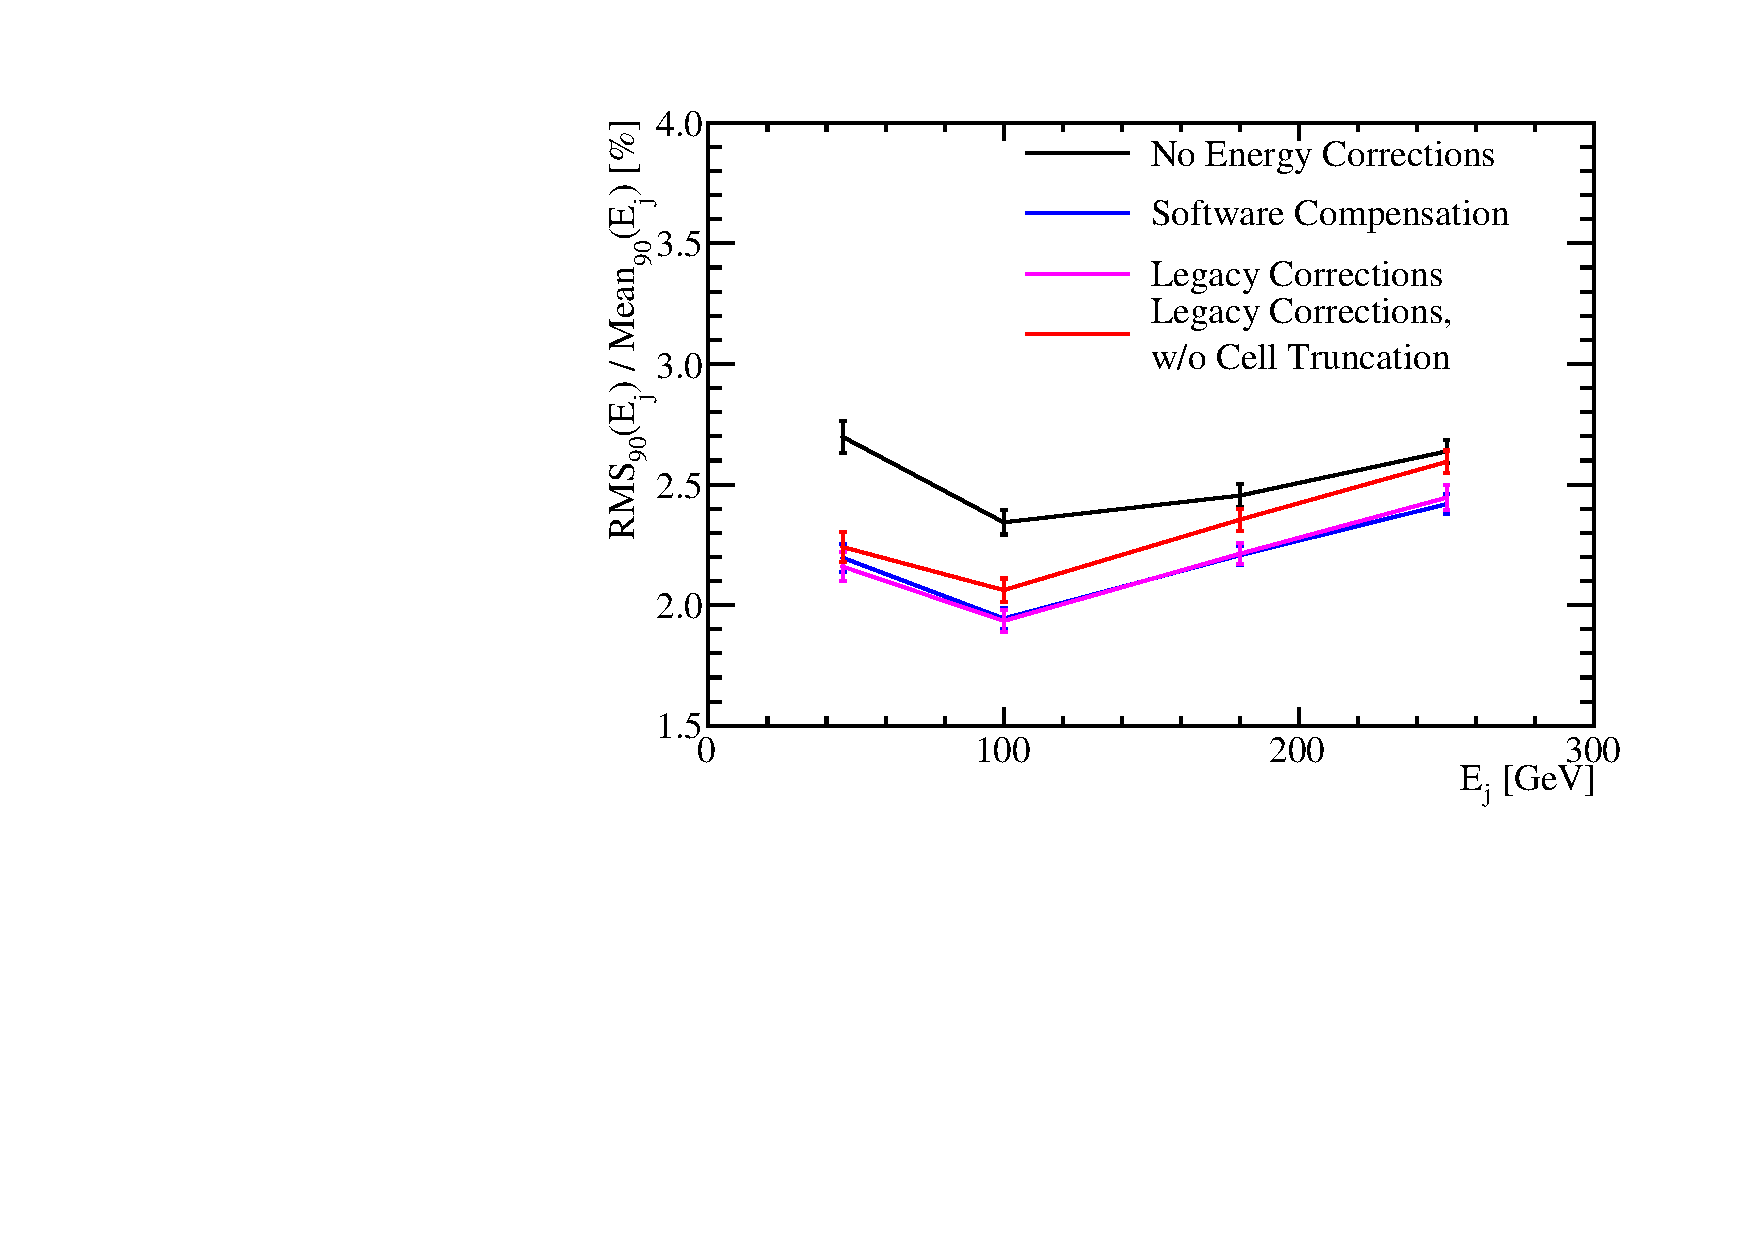
\includegraphics[width=0.5\textwidth]{EnergyEstimators/Plots/SoftComp/JetEnergyResolution/JER_vs_JetEnergy_TotalConfusion.pdf}}
\caption[The contributions to the jet energy resolution as a function of the jet energy for a variety of different energy correction options.  The jet energy resolution contributions presented are \protect\subref{fig:jerbreakdownsoftcomp1} the intrinsic energy resolution of the detector and \protect\subref{fig:jerbreakdownsoftcomp2} the total confusion contribution.  The jet energy resolution obtained using the standard reconstruction is given by the quadrature sum of the intrinsic energy resolution and total confusion contributions.  The black line represents no energy corrections, the blue line represents software compensation, the magenta line represents the legacy energy corrections and the red line represents the legacy corrections without the HCal hit energy truncation.  The nominal ILD detector model was used in these simulations.]{The contributions to the jet energy resolution as a function of the jet energy for a variety of different energy correction options.  The jet energy resolution contributions presented are \protect\subref{fig:jerbreakdownsoftcomp1} the intrinsic energy resolution of the detector and \protect\subref{fig:jerbreakdownsoftcomp2} the total confusion contribution.  The jet energy resolution obtained using the standard reconstruction is given by the quadrature sum of the intrinsic energy resolution and total confusion contributions.  The black line represents no energy corrections, the blue line represents software compensation, the magenta line represents the legacy energy corrections and the red line represents the legacy corrections without the HCal hit energy truncation.  The nominal ILD detector model was used in these simulations.}
\label{fig:jerbreakdownsoftcomp}
\end{figure}

%========================================================================================
%========================================================================================

\subsection{Summary}
The effect on both single particle and jet energy resolution of the HCal hit energy truncation and software compensation have been examined.  Although relatively simplistic, the HCal hit energy truncation was found to be beneficial for detector performance by limiting the impact of Landau fluctuations.  The more sophisticated software compensation procedure was found to be highly effective at producing a compensating calorimeter response across a wide range of energies, which translated into excellent performance in terms of jet energy resolution.

%========================================================================================
%========================================================================================

\section{Timing Cuts}
The linear collider will operate using trigger-less readout whereby the recorded data for each sub-detector is read out between collisions of the $\text{e}^{+}$ and $\text{e}^{-}$ bunches.  The bunch train structure for ILC and CLIC is compared in table \ref{table:trainstructure}.  Event selection will proceed through the application of a software trigger.  This involves the identification of any hard interactions, prior to full event reconstruction, and only putting data into the event reconstruction if it is measured within a chosen time window about these interactions.  The recorded time of a calorimeter hit, which is cut on to make the time window for the software trigger, is corrected for straight time-of-flight to the IP.  This ensures that the amount of time particle showers have to develop in the calorimeters is independent of their position in the detector.  The energy resolution of a calorimeter is sensitive to the choice of time window applied because energy measurements made outside the time window are rejected.  Therefore, the overall detector performance will be sensitive to the choice of time window used.  

At CLIC, the application of a software trigger is challenging because of the 0.5~ns bunch separation.  The small bunch separation means the integration time of the calorimeters will span many bunch crossings.  When this is combined with the intense beam-induced backgrounds, identification of energy deposits produced from a hard interaction of interest becomes difficult.  By placing tight timing constraints on the energy deposits made in the CLIC calorimeters, it is possible to minimise the impact of the beam-induced backgrounds.  As well as minimising the impact of the backgrounds, these tight timing requirements will also change how particle showers from the hard interaction of interest are sampled.  Understanding the impact of these timing requirements on physics performance is vital to the success of the CLIC experiment.  Application of the software trigger at the ILC is less challenging than at CLIC because the bunch separation is much larger, meaning the calorimeters could be read out between bunches, and the beam-induced backgrounds are much smaller.  

\begin{table}[h!]
\centering
\begin{tabular}{l r r}
\hline
& ILC 500~GeV & CLIC 3 TeV \\
\hline
Electrons per bunch [$10^{10}$] & 2.0 & 0.37 \\
Bunches per train & 2820 & 312 \\
Train repetition rate [Hz] & 5 & 50 \\
Bunch separation [ns] & 308 & 0.5 \\
\end{tabular}
\caption[The train structure for 500~GeV ILC and 3 TeV CLIC \cite{Behnke:2013lya,Linssen:2012hp}.]{The train structure for 500~GeV ILC and 3 TeV CLIC \cite{Behnke:2013lya,Linssen:2012hp}.}
\label{table:trainstructure}
\end{table}

For all choices of time window considered in this study the calibration procedure described in section \ref{sec:overviewcalibration} was reapplied.  This ensures that the \textit{mean} of the reconstructed energy distributions will not depend on changes in the calorimeter timing window because the calibration will compensate for any energy losses incurred by rejecting energy measurements made outside the time window.  

For the results presented in this chapter and the optimisation studies found in chapter \ref{chap:detopt}, a 100~ns timing window was applied to all detector models considered.  This value was chosen as it reflects particle shower development time \cite{Linssen:2012hp} and could be reasonably achieved using readout technology options presently available \cite{Adloff:2014rya}.  

%========================================================================================

\subsection{Impact on Single Particle Energy Resolution}
Figure \ref{fig:ertimingcuts} shows the energy resolution of the nominal ILD detector for 100~GeV photons and 50~GeV $K^{0}_{L}$s as a function of the timing window applied to the calorimeter hits.  The timing cut makes little difference to the energy resolution of photons, however, the energy resolution for neutral hadrons gets significantly worse as the time window is reduced.  The neutral hadron energy resolution becomes worse by almost 20~\% when the time window is reduced from $10^{6}$~ns to 10~ns.  These trends are to be expected because electromagnetic showers develop far more rapidly than their hadronic counterparts \cite{Wigmans:2000vf}.  This can be seen from figure \ref{fig:calohittiming}, which shows the distribution of the measurement time of calorimeter hits, corrected for time-of-flight, for selected shower components for 91~GeV Z$\rightarrow$uds events.  Hadronic showers develop more slowly as they often involve intermediate states that must decay to continue the propagation of the shower.  


If a narrow calorimeter timing window is used, energy measurements from the hadronic shower will be lost and the energy resolution will degrade, which is what is observed.  On the other hand, electromagnetic showers develop so rapidly that even the 10~ns time window does not reject many energy measurements. 

\begin{figure}[h!]
\subfloat[]{\label{fig:ertimingcutsphotons}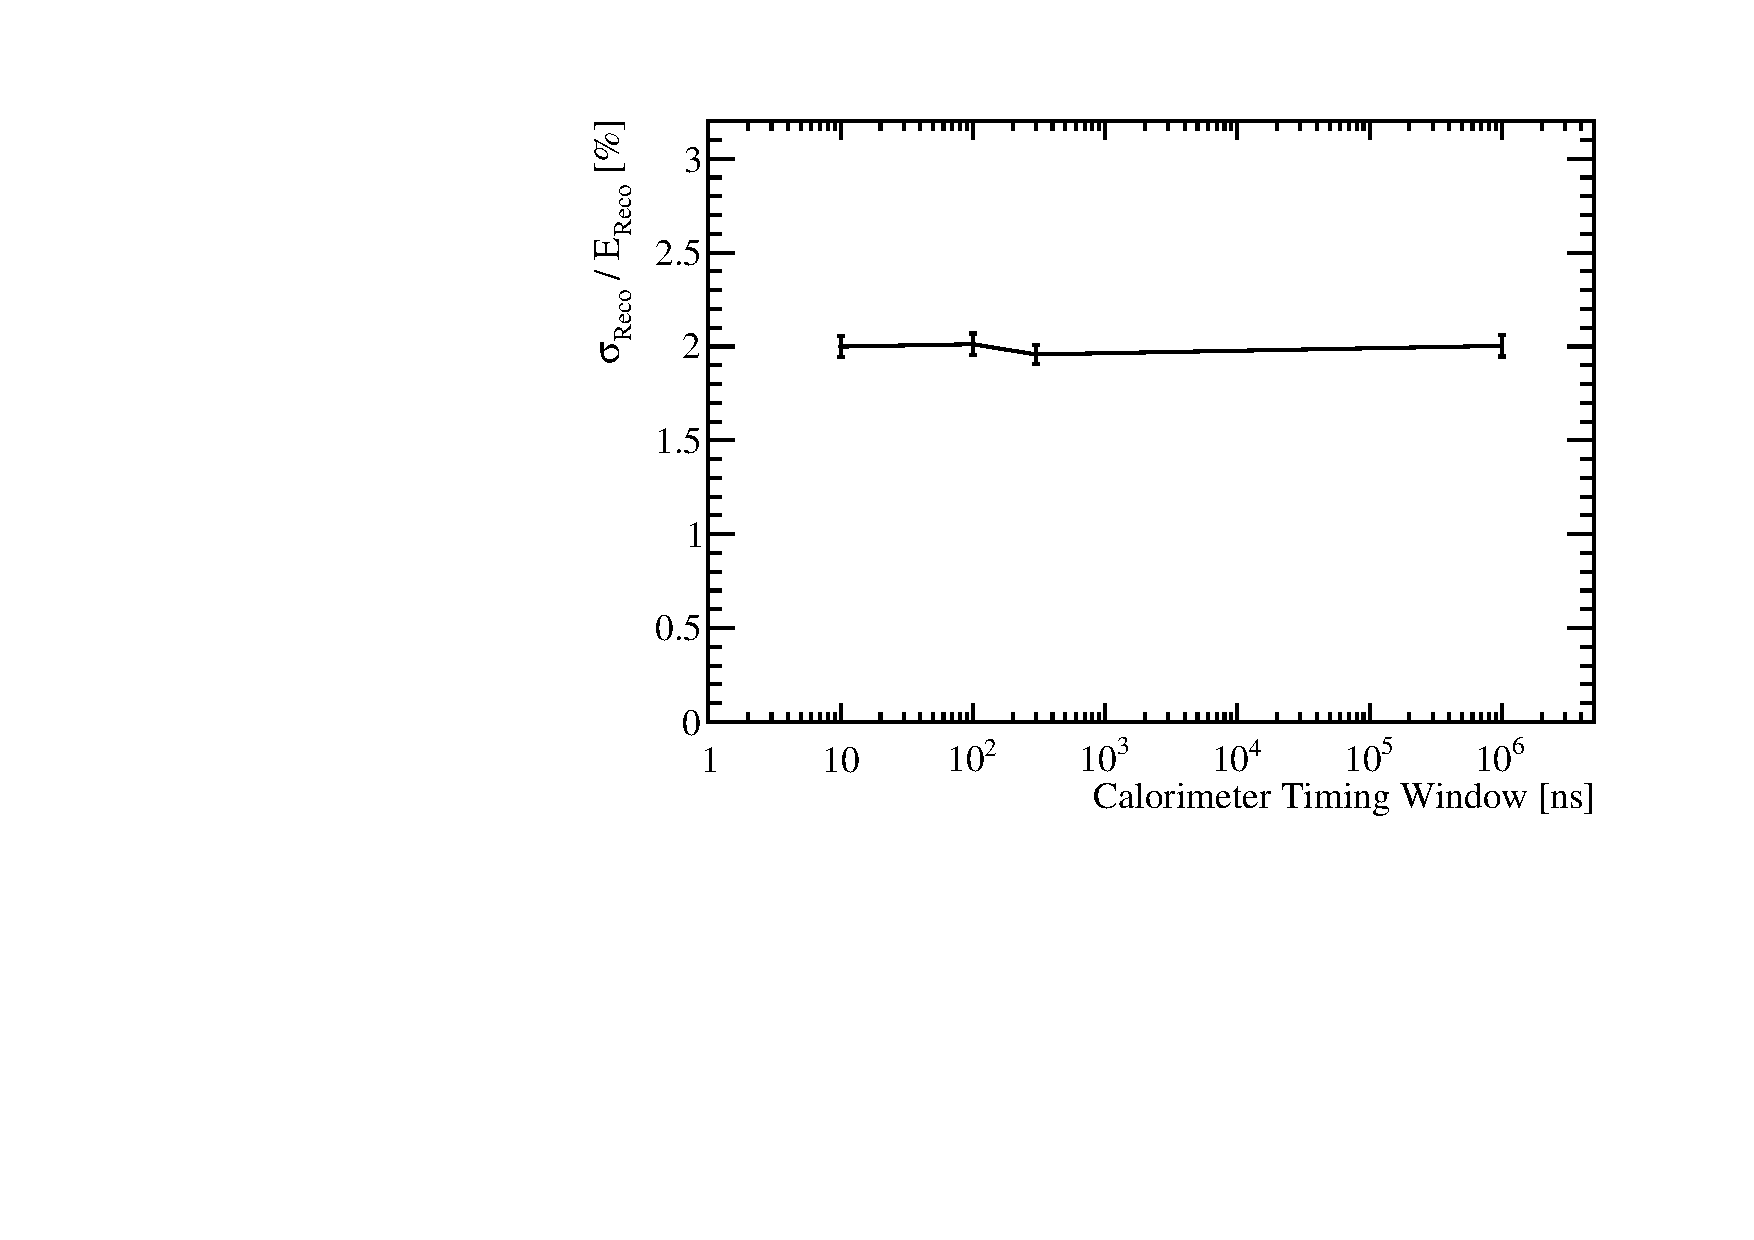
\includegraphics[width=0.5\textwidth]{EnergyEstimators/Plots/TimingCuts/ER_vs_PhotonTiming_100GeVPhoton.pdf}}
\subfloat[]{\label{fig:ertimingcutskaons}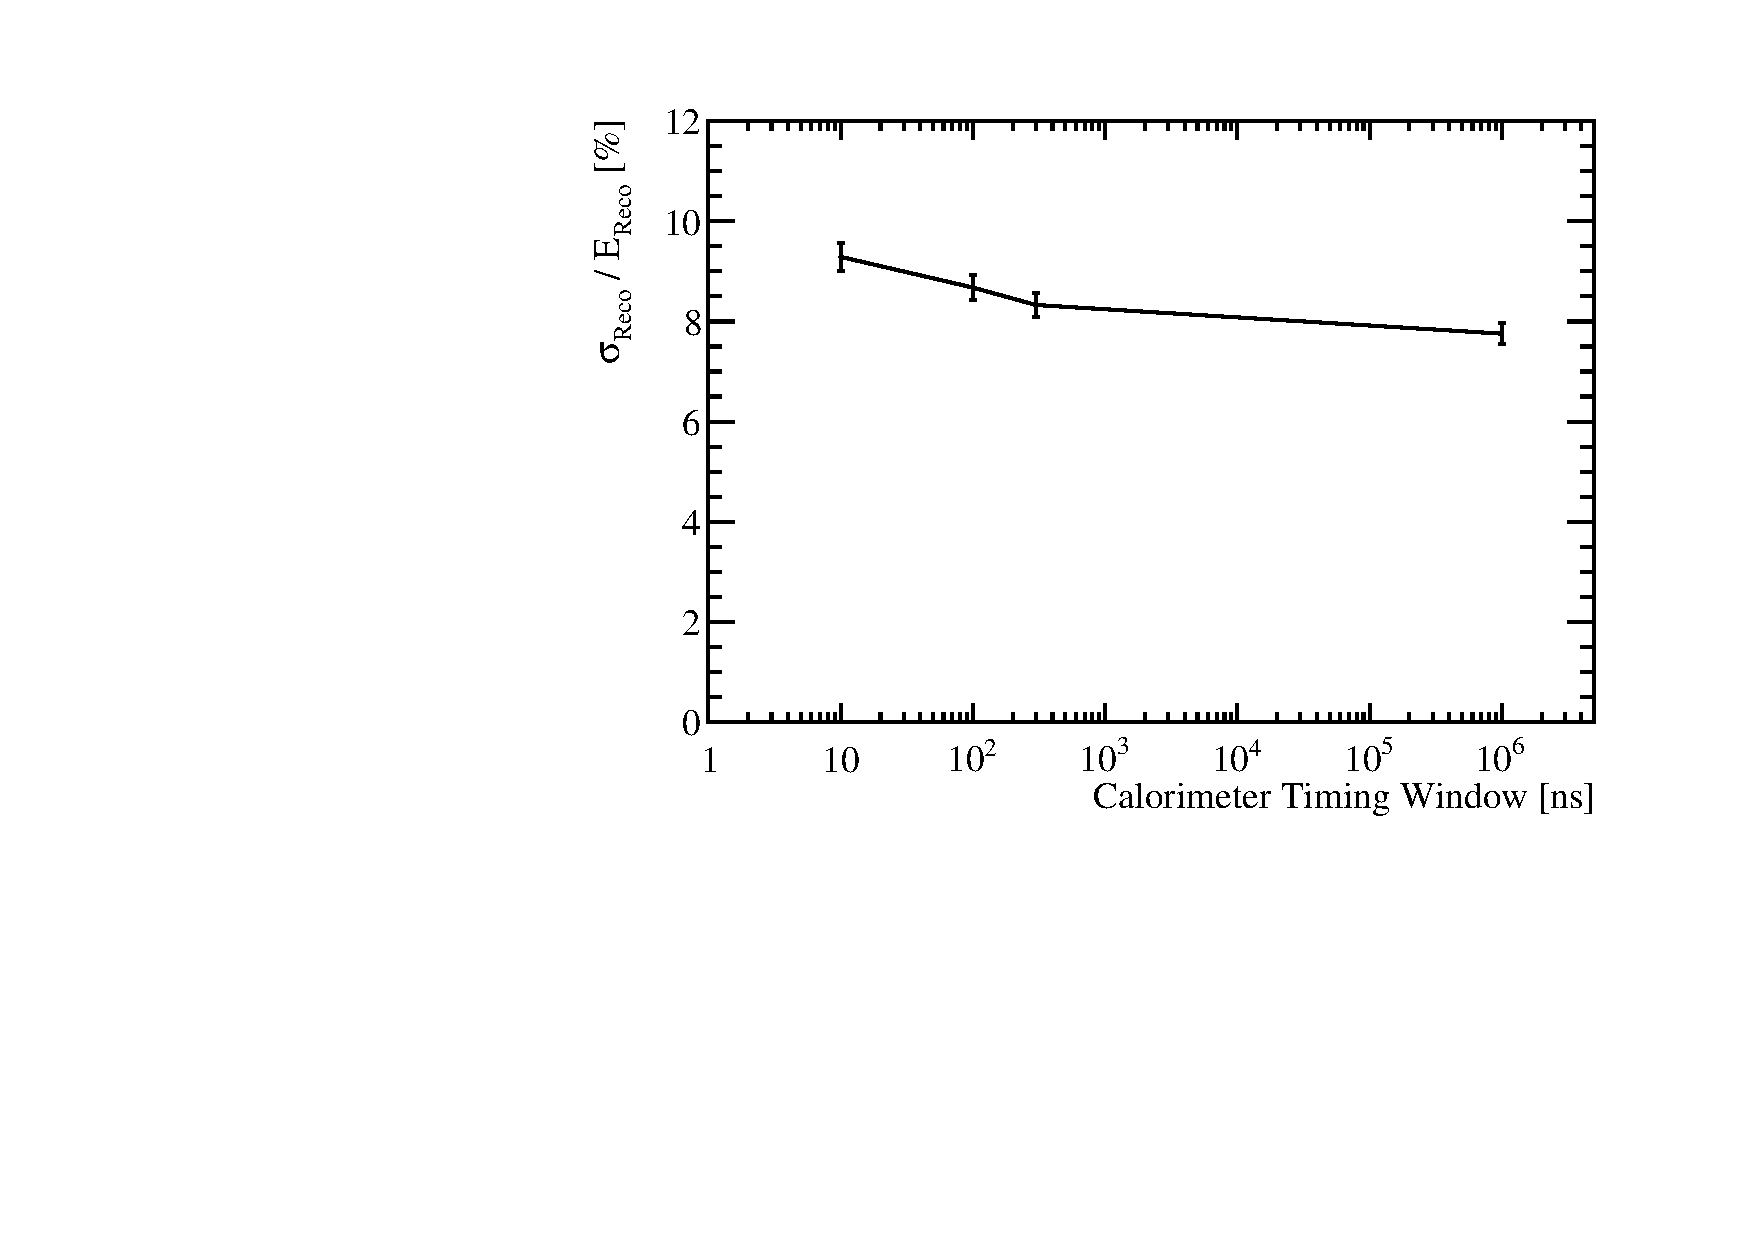
\includegraphics[width=0.5\textwidth]{EnergyEstimators/Plots/TimingCuts/ER_vs_Kaon0LTiming_50GeVKaon0L.pdf}}
\caption[The energy resolution as a function of calorimeter timing window for \protect\subref{fig:ertimingcutsphotons} 100~GeV photons and \protect\subref{fig:ertimingcutskaons} 50~GeV $K^{0}_{L}$ events using the nominal ILD detector model.]{The energy resolution as a function of calorimeter timing window for \protect\subref{fig:ertimingcutsphotons} 100~GeV photons and \protect\subref{fig:ertimingcutskaons} 50~GeV $K^{0}_{L}$ events using the nominal ILD detector model.}
\label{fig:ertimingcuts}
\end{figure}

\begin{figure}[h!]
\centering
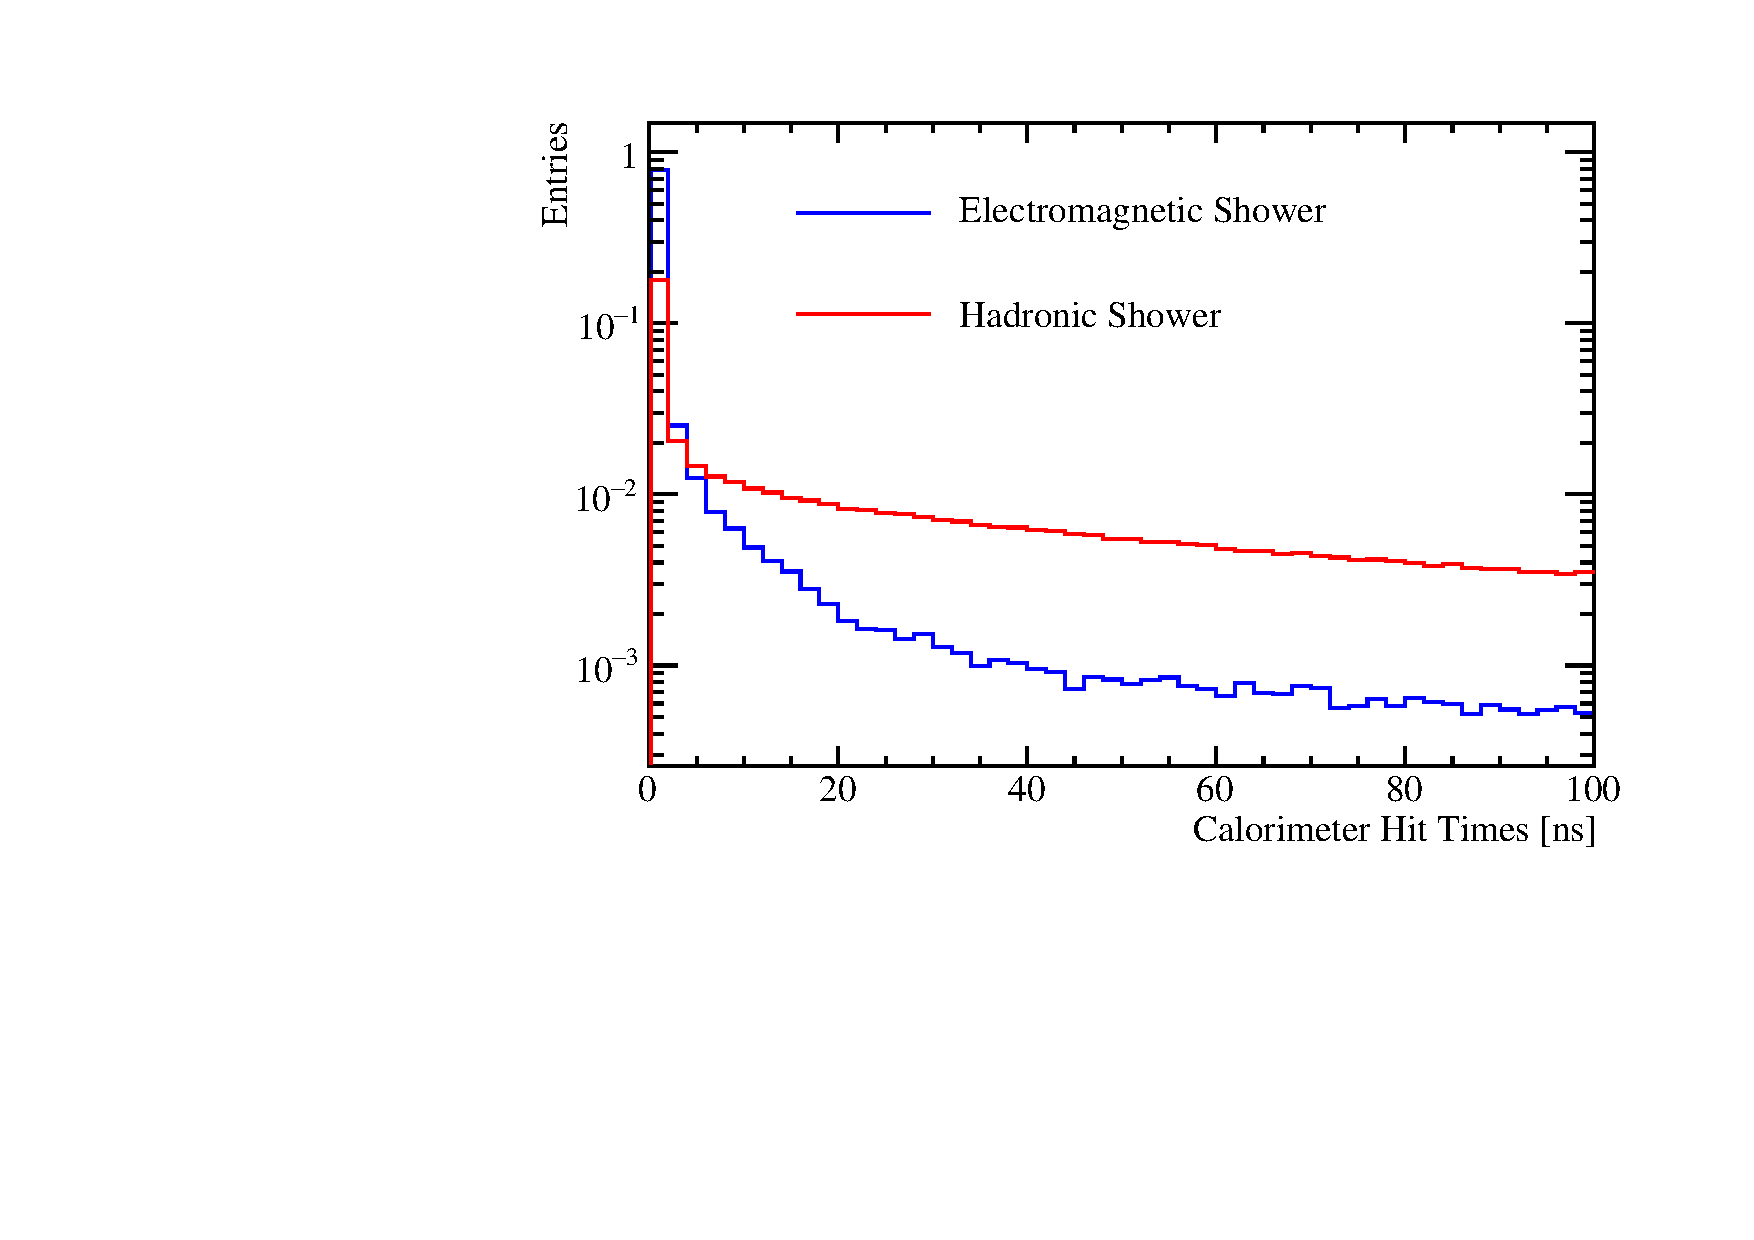
\includegraphics[width=0.75\textwidth]{OptimisationStudies/Plots/Description/CalorimeterHitTimes_91GeV_Z_uds_Steel_Normalised.pdf}
\caption[The normalised distribution of the time of the electromagnetic and hadronic shower calorimeter hits, corrected for time of flight to the impact point, for 91~GeV Z$\rightarrow$uds events.  Electromagnetic shower energy deposits are deposited very rapidly, while hadronic shower energy deposits are deposited over a much longer time period.]{The normalised distribution of the time of the electromagnetic and hadronic shower calorimeter hits, corrected for time of flight to the impact point, for 91~GeV Z$\rightarrow$uds events.  Electromagnetic shower energy deposits are deposited very rapidly, while hadronic shower energy deposits are deposited over a much longer time period.}
\label{fig:calohittiming}
\end{figure} 

%========================================================================================

\subsection{Impact on Jet Energy Resolution}
Figure \ref{fig:jertimingcuts} shows the jet energy resolution as a function of the jet energy for selected calorimeter time windows.  As expected, the jet energy resolution becomes worse when the calorimeter timing window is reduced.  

\begin{figure}[h!]
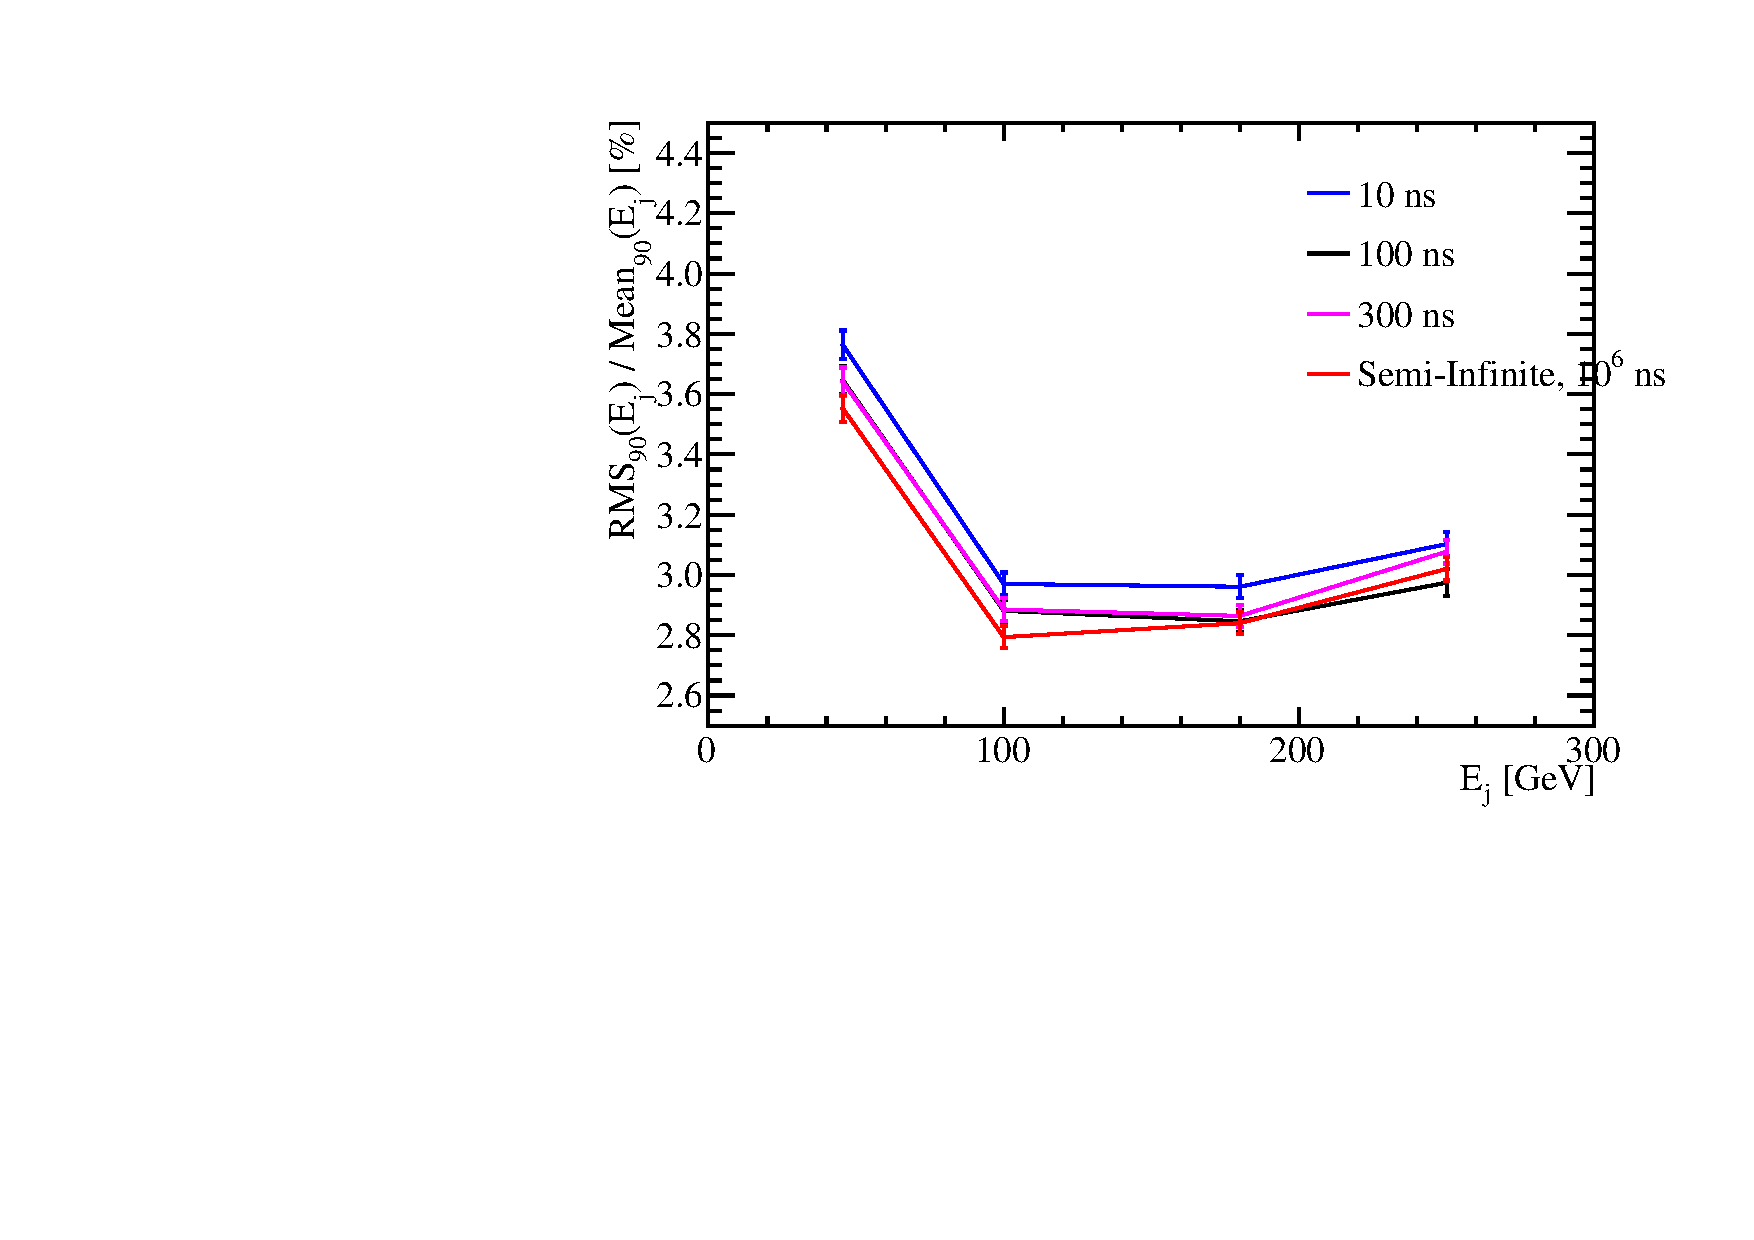
\includegraphics[width=0.5\textwidth]{EnergyEstimators/Plots/TimingCuts/JER_vs_JetEnergy_TimingCutStudies.pdf}
\caption[The jet energy resolution as a function of jet energy for various calorimeter timing cuts.  The nominal ILD detector model was used in these simulations.]{The jet energy resolution as a function of jet energy for various calorimeter timing cuts.  The nominal ILD detector model was used in these simulations.}
\label{fig:jertimingcuts}
\end{figure}

The time window applied to the calorimeter hits affects both the neutral hadron and jet energy resolutions with a larger timing window leading to better resolutions.  It can be seen that by applying an aggressive choice of time window, such as 10~ns, the jet energy resolution would be degraded because many of the hadronic showers are not fully sampled.  However, even using a 10~ns timing cut the jet energy resolutions are still sufficiently low to give excellent detector performance.  Both the single particle and jet energy resolutions indicate that the majority of hadronic showers at the energies considered will be fully sampled using a 100~ns time window and that there is little to be gained by increasing this time window further.

%========================================================================================

\subsection{Summary}
Simulations were performed to study the impact of the calorimeter hit time window used in the software trigger at the linear collider experiments.  The energy resolution for electromagnetic showers did not change significantly when varying the size of time window, however, the neutral hadron energy resolution becomes worse as the size of the time window is reduced.  The jet energy resolution is also sensitive to the size of the time window used, however, the trend was far weaker than that seen for neutral hadrons because only 10\% of the jet energy is carried in the form of neutral hadrons.  Increasing the time window beyond 100~ns did not have any significant benefit indicating that the majority of hadronic shows are fully sampled in this time.   

%========================================================================================
%========================================================================================
